\documentclass[12pt]{yalephd}
% See here for more detailed guidelines on dissertation format
% https://gsas.yale.edu/sites/default/files/formatdissertation.pdf


\usepackage{graphicx}
% Chapters under PHIL/ reference their images as figures/xxx.png
\graphicspath{{./}{PHIL/}{HYBRID/}}
\usepackage{lscape}
\usepackage{times}
\usepackage{float}
\usepackage{amssymb,amsmath}
\usepackage{algorithm2e}
\usepackage{float}
\usepackage{subcaption}
\usepackage{afterpage}
%\usepackage{natbib}
\usepackage{epsfig}
\usepackage{longtable}
\usepackage[pagebackref=true]{hyperref}
\usepackage{hyperref}
\usepackage[dvipsnames]{xcolor}
\usepackage{setspace}
\usepackage{titlesec}
\definecolor{linkColor}{rgb}{0.,0.11,0.22}
\definecolor{YaleBlue}{rgb}{0.0,0.22,0.444}
\usepackage{natbib}
% Packages and macros needed by the chapters under PHIL/
% (extracted from the original paper preamble, PHIL/appendix.tex)

% T1 encoding: accented letters (ö in "Teichteil-Königsbuch") become single
% glyphs, so TeX can hyphenate the word instead of overflowing the margin.
\usepackage[T1]{fontenc}

\usepackage{booktabs}           % professional-quality tables
\usepackage{multirow}           % tabular cells spanning multiple rows
\usepackage{multicol}
\usepackage{amsfonts}           % blackboard math symbols
\usepackage{array}
\usepackage{wrapfig}
\usepackage{nicefrac}           % compact symbols for 1/2, etc.
\usepackage{url}
\usepackage{enumitem}
\usepackage{xspace}
\usepackage[mathscr]{euscript}
\usepackage[export]{adjustbox}

% Author-annotation helpers
\newcommand{\rex}[1]{{{\textcolor{magenta}{[rex: #1]}}}}
\newcommand{\jure}[1]{{{\textcolor{red}{[Jure: #1]}}}}
\newcommand{\michal}[1]{{{\textcolor{blue}{[Michal: #1]}}}}
\newcommand{\update}[1]{{{\textcolor{ForestGreen}{[Update: #1]}}}}

% Shorthands
\newcommand{\etal}{\textit{et al.}\xspace}
\newcommand{\alg}{\textsc{PHIL}\xspace}
\newcommand{\sail}[0]{\textsc{SaIL}\xspace}
\newcommand{\VS}{\mathcal{V}}
\newcommand{\xhdr}[1]{{\noindent\bfseries #1}.}

% Math
\DeclareRobustCommand{\bbone}{\text{\usefont{U}{bbold}{m}{n}1}}
\DeclareMathOperator{\EX}{\mathbb{E}} % expected value

% algorithm2e configuration (package itself is loaded in Disseration.tex)
\SetKwComment{Comment}{$\triangleright$\ }{}
\newcommand{\algorithmStyle}[0]{\footnotesize}


%%%%%%%%%%%%%%%%%%%%%%%%%%%%%%%%%%%%%%%%%%%%%%%%%%%%%%%%%%%%%%%%%%%%%%%%%%%%%%%
% HyBRiD chapter (from the ICML 2024 paper preamble)
%%%%%%%%%%%%%%%%%%%%%%%%%%%%%%%%%%%%%%%%%%%%%%%%%%%%%%%%%%%%%%%%%%%%%%%%%%%%%%%

\usepackage{mathtools}
\usepackage{amsthm}
\usepackage{tabularx}
\usepackage{caption}
\usepackage{pifont}
\usepackage{bbm}                % \mathbbm
\usepackage{microtype}
\usepackage[textsize=tiny]{todonotes}
\usepackage[capitalize,noabbrev]{cleveref}   % load last

% Theorem environments (numbered per chapter, not per section, in a book class)
\theoremstyle{plain}
\newtheorem{theorem}{Theorem}[chapter]
\newtheorem{proposition}[theorem]{Proposition}
\newtheorem{lemma}[theorem]{Lemma}
\newtheorem{corollary}[theorem]{Corollary}
\theoremstyle{definition}
\newtheorem{definition}[theorem]{Definition}
\newtheorem{assumption}[theorem]{Assumption}
\theoremstyle{remark}
\newtheorem{remark}[theorem]{Remark}

% Table rules/struts used by the HyBRiD tables
\newcommand{\Tstrut}{\rule{0pt}{2.9ex}}         % "top" strut
\newcommand{\Bstrut}{\rule[-1.2ex]{0pt}{0pt}}   % "bottom" strut
\newcommand{\TBstrut}{\Tstrut\Bstrut}
\newcommand{\shline}{\addlinespace[3pt]\hline\addlinespace[3pt]}

% Names
\newcommand{\mname}{\textsc{HyBRiD}}
\newcommand{\multiheadname}{\textit{multi-head drop-bottleneck}}
\newcommand{\avgimp}{$12.1\%$}

% Review annotations (\rex is defined above and deliberately not redefined)
\newcommand{\htl}[1]{\textcolor{orange}{[htl: #1]}}
\newcommand{\yize}[1]{\textcolor{magenta}{[Yize: #1]}}
\newcommand{\jialin}[1]{\textcolor{brown}{[jialin: #1]}}
\newcommand{\sw}[1]{{\color{magenta}***SW: #1***}}
\newcommand{\cam}[1]{{\color{red}#1}}


%%%%%%%%%%%%%%%%%%%%%%%%%%%%%%%%%%%%%%%%%%%%%%%%%%%%%%%%%%%%%%%%%%%%%%%%%%%%%%%
% MindLLM chapter (from the ICML 2025 paper preamble)
%%%%%%%%%%%%%%%%%%%%%%%%%%%%%%%%%%%%%%%%%%%%%%%%%%%%%%%%%%%%%%%%%%%%%%%%%%%%%%%
% Packages already loaded above are not repeated: mathtools, amsthm, tabularx,
% caption, pifont, cleveref, adjustbox, multicol, enumitem, array, subcaption.
% The paper's `subfigure` package is deliberately NOT loaded — it clashes with
% subcaption, and only the subcaption `subfigure` *environment* is used.
% Theorem environments are shared with the HyBRiD block above.

\usepackage{makecell}
\usepackage{siunitx}
\usepackage[normalem]{ulem}     % \uline
\usepackage[most]{tcolorbox}

% Names and marks
\newcommand{\mindllm}{MindLLM}  % the paper's \name, renamed to avoid a clash
\newcommand{\cmark}{\ding{51}}
\newcommand{\xmark}{\ding{55}}
\newcommand{\tdag}{\textsuperscript{\textdagger}}

% Review annotations (\rex is defined above and deliberately not redefined)
\newcommand{\yy}[1]{\textcolor{orange}{(Yujun: #1)}}
\newcommand{\qwk}[1]{\textcolor{blue}{(Weikang: #1)}}


%%%%%%%%%%%%%%%%%%%%%%%%%%%%%%%%%%%%%%%%%%%%%%%%%%%%%%%%%%%%%%%%%%%%%%%%%%%%%%%
% PRISM chapter (from the ICLR 2026 paper preamble)
%%%%%%%%%%%%%%%%%%%%%%%%%%%%%%%%%%%%%%%%%%%%%%%%%%%%%%%%%%%%%%%%%%%%%%%%%%%%%%%
% The paper's math_commands.tex defines 431 macros, none of which the chapters
% use, so it is not merged. Its `algorithm`/`algorithmic` packages are also
% skipped: no algorithm environment is used, and they would clash with the
% algorithm2e loaded for the PHIL chapter.

\newcommand{\modelname}{\textbf{{PRISM}}\xspace}


%%%%%%%%%%%%%%%%%%%%%%%%%%%%%%%%%%%%%%%%%%%%%%%%%%%%%%%%%%%%%%%%%%%%%%%%%%%%%%%
% RepQA chapter (from the npj Digital Medicine paper preamble)
%%%%%%%%%%%%%%%%%%%%%%%%%%%%%%%%%%%%%%%%%%%%%%%%%%%%%%%%%%%%%%%%%%%%%%%%%%%%%%%
% \bench is the only macro from that preamble the chapter actually uses; the
% rest (\model, \Set, \Mat, \vpara, \reb, \xm, \xp, prop/problem theorems) and
% its heavy packages (commath, listings, subfigure, threeparttable, lineno) go
% unused, so they are not merged. \rex/\htl already exist above.
\newcommand{\bench}{\textsc{RepQA}\xspace}

% A part-divider page that carries a short introductory paragraph on the SAME
% page as the part title (the book class would otherwise push the intro onto
% the following page). Usage: \partwithintro{Part title}{Intro paragraph...}
\makeatletter
\newcommand{\partwithintro}[2]{%
  \begingroup
    % Suppress the automatic \vfil\newpage that book.cls fires right after the
    % part title, so the introduction can share the part page.
    \renewcommand\@endpart{}%
    \part{#1}%
  \endgroup
  \vskip 2.5em
  \begin{quote}#2\end{quote}%
  \vfil            % balances the \null\vfil book.cls put before the title,
  \newpage         % centering the title+intro block vertically on the page.
}
\makeatother

% Last-resort stretch for paragraphs TeX cannot otherwise break — these papers
% were set in two columns and some have long unbreakable inline math that now
% overflows the wider one-column measure. Only applies where a line would
% otherwise stick out; well-set paragraphs are untouched.
\emergencystretch=3em


\begin{document}

\newcommand{\unit}[1]{\ensuremath{\, \mathrm{#1}}}

\titleformat{\chapter}[display]
    {\fontfamily{ptm}\huge\bfseries}{\chaptertitlename\ \thechapter}{5pt}{\centering\singlespacing\huge}% NEW
\titlespacing*{\chapter}{0pt}{50pt}{30pt}% NEW

	% Dissertation Title: Subtitle
	\title{Yale Sample Thesis Template}
	% Full Name of Author (as it should appear on the diploma)
	\author{Full Name of Author}
	%
	% where there is an advisory committee, only the chairperson is listed
	\advisor{Full Name of the Advisor(s)}
	% Month and Year Degree is to be awarded
    % (not the month where the dissertation is submitted)
	\date{Month Year}

%	\singlespace

    % Abstract. The 2026 Registrar guide sets no word limit; it requires the
% heading, title, author and conferral year above the text (all supplied by the
% abstract environment in yalefmt.tex), double spacing, and page number "iii".
\begin{abstract}

In contemporary machine learning systems, language often mediates interaction between people and modalities. Text-to-image generators, vision-language models, and voice assistants, for example, assume that human intent can be expressed in words before the system interprets or acts on it. Yet verbal expression is serial and limited in bandwidth, and some mental content is difficult to put into words. RepQA, our benchmark for patient education question answering, provides a narrower motivation from the system side: methods can improve readability, but simplified answers may still omit important content. These limitations motivate this dissertation to explore a complementary interface between mind and world that does not require people to articulate their intent first. This problem divides into three questions: (1) how can machine learning uncover neural organization that is not specified in advance, and how can established neural priors in turn be built into machine-learning models; (2) what representation space and structure can best connect brain activity to the world, and how can the necessary supervision be assembled when neural data are scarce; and (3) how can human intention be connected to behavior in the world?

For the first question, we study a two-way exchange between machine learning and neural priors: machine learning can discover neural organization that is not specified in advance, while established neural organization can guide the design of machine-learning models. HyBRiD realizes the first direction by learning outcome-relevant, high-order relationships among brain regions as weighted hyperedges rather than restricting connectivity to pairwise edges; a multi-head drop-bottleneck makes a maximally-informative-minimally-redundant objective tractable, allowing the hyperedges to be learned end-to-end instead of enumerated and pruned in advance. In the other direction, our neuro-informed attention encoder aggregates subject-specific sets of responsive voxels with learnable queries, while its keys contain only voxel position and multi-atlas parcellation embeddings, separating measured fMRI activity from spatial and parcellation priors that can be shared across subjects. FA-EEG likewise uses frame averaging to make the known mirror symmetry between left and right motor imagery exact for any backbone rather than relearning it from scarce trials. This transfer from neuroscience to machine learning also extends beyond models of neural signals: SWA identifies small-world organization in functional networks of language-model attention heads, relates that organization to fluid reasoning, and preserves it when allocating sparsity during pruning.

For the second question, the argument follows alignment-space selection, alignment learning, language-mediated reconstruction, and a more expressive disentangled generator. PRISM I compares candidate alignment spaces and finds that, among those tested, fMRI aligns more closely with language-model semantic representations than with the visual latents conventionally used for reconstruction. MindLLM learns fMRI-to-language alignment through brain instruction tuning, which creates supervision without new scanning by joining fMRI recordings to a decade of existing annotations through their shared stimulus images. The resulting corpus of 980{,}610 conversations spans four families of brain function: perception, memory and knowledge, language and symbols, and complex reasoning. A decoder trained on this corpus answers open-ended questions in a unified format, improves general decoding, and generalizes to a held-out subject without finetuning. PRISM II uses language for visual reconstruction, structuring the representation into objects, attributes, and relations and generating scenes object by object. This object-disentangled space motivates stronger separation between items in the generator itself. \dedit{} extends the generative side beyond object-centric scene construction by learning one prompt per image item and using grouped cross-attention to confine each region to its associated prompt. This enables broader item-level control through text-, mask-, and reference-image-guided editing and object removal; integration with a neural decoder remains future work.

For the third question, the argument progresses from action meaning to goal realization. At the action level, the Mind World Model jointly learns a mind model that encodes EEG as latent actions and a world model that predicts their visual consequences in synchronized egocentric video. This prediction objective, together with cross-modal alignment, connects brain signals to action intention without trial or action labels. The EEG-derived code also turns adjacent video frames into action-conditioned training examples without recorded actions; because it is computed without access to the target frame, it prevents the action channel from simply carrying the future observation. Task completion often calls for specifying the desired outcome rather than each action, motivating the move to goal-directed planning and policies. At this goal level, PHIL and DySta offer complementary interfaces corresponding to the images and text of the semantic bridge. In the dissertation's embodiment framing, PHIL searches toward a graph state representing the outcome depicted in a goal image, using learned node-to-goal distance heuristics. DySta generates actions directly from a language instruction and multi-frame visual history. It separates visual tokens by temporal persistence, retains a single copy and KV cache for static tokens, and refreshes them through a learned recache gate, combining effective task completion with efficient inference. The three models are evaluated independently; connecting decoded representations to these goal interfaces remains future work.

\end{abstract}

	
    \maketitle
    \makecopyright
	
    \begin{center}
{\bf \large Acknowledgments}
\end{center}


Thanks my advisor Prof Rex Ying for his guidance and support throughout my PhD journey. I am also grateful to my committee members for their valuable feedback and insights.


Thanks my committe members Prof. Arman Cohan, Prof. David van Dijk, Prof. Yujun Yan.


Thanks my labmates Tinglin Huang, Jialin Chen, Yangtian Zhang.


Thanks the people who drink alcohol with me regularly.


Thanks my father and mother.
	
    \tableofcontents % 
    \listoffigures   % The standard LaTeX form works well.
    \listoftables    % 
    
    \mainmatter      % Reset the pagenumbering options

	\chapter{Introduction}
\label{chapter:introduction}

\section{Motivation}

Language has become a common interface between people and multimodal machine learning systems. Modern models can process information across text, images, audio, and video~\citep{han2024onellm,radford2021learning,liu2023visual}, yet many systems use words to connect these modalities. In text-to-image generation, users describe the desired result with a prompt~\citep{rombach2022high}; in vision-language models, users ask questions about images and receive answers in language~\citep{liu2023visual}; and in voice assistants, spoken instructions are translated into actions. This design is natural and useful, but it raises a basic question: \emph{Is this the most effective and efficient way?}

Language is powerful, but it can also be a narrow channel. Expression unfolds sequentially, so a person may have to compress a rich intention into a short prompt and then refine it through several rounds of feedback. Some experiences are even harder to verbalize. The abstract structure and affective intensity of Wassily Kandinsky's \emph{Composition VII}, for example, can be perceived as a whole but are difficult to capture precisely in words. Together, these limitations motivate a complementary channel through which some percepts, intentions, or internal states can be communicated without deliberate verbalization.

The same limitation can appear in the opposite direction, when a machine communicates with a person. In patient education, an answer is useful only if a lay reader can understand it without losing essential information. The models evaluated in \repqa, introduced in Chapter~\ref{chapter:repqa}, often miss a requested reading level, while interventions that improve readability can omit part of the original content.

Motivated by these observations, this dissertation develops machine learning methods for a more direct interface between mind and world. These methods model neural signals, connect them to semantic and perceptual representations, and investigate how action meaning can be learned from neural activity and how embodied systems can realize specified goals. Language may still serve as an internal representation or output format; the goal is to reduce the need for a person to formulate every intention as a verbal instruction.

Such an interface could matter in three ways. First, models that identify meaningful patterns in neural activity can help reveal how distributed brain systems support perception, cognition, and behavior. They may also support clinical analysis by characterizing disease-related network changes, predicting treatment response, and evaluating rehabilitation-related neural changes, as investigated respectively in Alzheimer's disease, depression, and multiple sclerosis~\citep{li2015toward,siegle2006use,cerasa2013computer}. Second, neural decoding could make aspects of internal thought, mental imagery, and dreams available in a form that can be inspected and shared. Text could provide a readable account of decoded semantic content, while images could convey visual appearance and spatial relationships. For example, externalizing an imagined scene could provide a starting point for creative work, and recovering aspects of dream imagery could offer material for studying subjective experience. Third, decoded neural signals could provide commands or goals to external systems. Speech neuroprostheses and a neurally controlled robotic arm already show how neural signals can support communication and device control for people with speech or motor impairments~\citep{card2024accurate,hochberg2012reach}; in the longer term, decoded intentions could also guide other assistive devices and embodied agents.

Realizing this interface raises three fundamental challenges. (1) \emph{Understanding the brain} requires a two-way exchange: machine learning must discover neural structure that is not specified in advance, while principles of neural organization can guide the analysis and design of machine learning models. (2) \emph{Decoding brain states} requires identifying which candidate representation is well aligned with neural activity and learning that mapping across subjects and tasks from limited paired data to recover content as text or images. (3) \emph{Enabling interaction} moves from action meaning to goal realization: how can neural representations acquire meaning through actions and their consequences, and how can a person specify a desired outcome while an embodied agent determines how to achieve it effectively and efficiently?

\section{Contributions}

This dissertation addresses these challenges through studies of neural modeling, semantic and perceptual representations, and embodied interaction. Across these studies, each model exploits structure specific to its problem: brain connectivity and anatomy, objects and relations in decoded scenes, and temporal persistence or graph topology in control and search. The main contributions are grouped as follows:

\begin{itemize}
    \item \textbf{Connecting neural organization and model design.} I use machine learning to identify candidate patterns of brain organization and draw on neuroscience to study the organization of language models. \hybrid{} learns candidate outcome-relevant, high-order relationships among brain regions instead of restricting analysis to pairwise connections. Small-World Allocation (SWA) uses the functional organization of attention heads to guide pruning, translating a principle studied in brain networks into a method for preserving language model performance (Chapters~\ref{chapter:hybrid} and~\ref{chapter:swa}).

    \item \textbf{Building a language bridge from fMRI alignment to disentangled visual generation.} The argument begins with \prism{} I, whose comparison of candidate representation spaces motivates language as an alignment target for fMRI. \mindllm{} then learns fMRI-to-language alignment across subjects and tasks, combining a neuroscience-informed encoder with Brain Instruction Tuning: the encoder incorporates voxel location and brain parcellations, while instruction tuning expands supervision through existing annotations linked by shared stimulus images. \prism{} II examines how language can support visual reconstruction by structuring the representation into objects, attributes, and relations and composing scenes object by object. This object-disentangled space motivates \dedit{}, which strengthens the generator's item-level disentanglement through learned per-item prompts and grouped cross-attention, enabling broader visual control. These contributions connect space selection, alignment learning, language-mediated reconstruction, and a more expressive disentangled generator (Chapters~\ref{chapter:prism}--\ref{chapter:dedit}).

    \item \textbf{Moving from action meaning to goal-directed behavior.} I study how intention can become behavior, progressing from the action level to the goal level. The Mind World Model (\mwm{}) jointly learns a mind model that encodes EEG as latent actions and a world model that predicts their visual consequences in synchronized egocentric video, connecting brain signals to action intention without action annotations. Completing a task often calls for specifying the desired outcome rather than each action, motivating two complementary approaches to goal realization. Their interfaces are a goal image for \phil{} and a language instruction for \dysta{}, corresponding to the images and text decoded in Part~\ref{part:bridge}. \phil{} learns graph-search heuristics for a target state representing the outcome specified by the image. \dysta{} generates actions from the language instruction and multi-frame visual history, using static--dynamic disentanglement to improve task success and inference efficiency. These independently evaluated studies connect the research questions of learning action meaning and acting toward a desired result (Chapters~\ref{chapter:mwm}--\ref{chapter:dysta}).
\end{itemize}

My long-term goal is to develop an additional communication channel between people and machines, especially when speech is impossible, too slow, or unable to preserve the relevant content. The present work recovers only task-dependent aspects of neural activity and does not yet integrate neural decoding with robotic control. It develops the main components separately: neural modeling, representation learning, control, and planning.

\section{Thesis Outline}

The dissertation begins with a prologue and then proceeds in three parts: the foundation for modeling brain signals, the bridge from signals to representations, and the study of action meaning and goal realization for embodied interaction.

\textbf{Prologue.} Chapter~\ref{chapter:repqa} introduces \repqa, a benchmark for evaluating readability in patient education question answering. The chapter asks whether large language models can write at a requested reading level, infer the level required by a question, and improve readability without sacrificing informativeness. The results show that the models often fail to meet requested reading levels and that readability-oriented post-training can discard useful content. This chapter provides a concrete example of information being lost in the machine-to-human direction and motivates the search for complementary interfaces.

\textsc{Part~\ref{part:foundation}} examines the relationship between neural organization and machine learning. Its two chapters discover high-order structure in brain signals and apply a principle from neuroscience to language model analysis and pruning.

Chapter~\ref{chapter:hybrid} introduces \hybrid{}, a method for identifying candidate high-order relationships among brain regions. Existing approaches usually represent functional connectivity with pairwise edges or select higher-order candidates before learning, which can miss distributed patterns that matter for cognition. \hybrid{} instead represents these relationships as weighted hyperedges and learns them end to end through a maximally-informative-minimally-redundant objective and a multi-head drop-bottleneck. The learned hyperedges improve phenotypic prediction, while post-hoc analyses suggest that higher-degree hyperedges carry useful phenotypic information.

Chapter~\ref{chapter:swa} studies whether the small-world organization observed in functional brain networks also provides insight into language models. It constructs functional graphs whose nodes are attention heads and whose edges reflect activation similarity. Across the evaluated models, stronger small-world organization was associated with better fluid reasoning performance. SWA uses scores for within-community and cross-community connectivity to allocate sparsity across heads and layers, preserving this organization and improving performance under pruning.

\textsc{Part~\ref{part:bridge}} develops the bridge from brain signals to visual content through a connected argument: \prism{} I informs the choice of alignment space; \mindllm{} learns fMRI-to-language alignment; \prism{} II uses language for visual reconstruction; and the object-disentangled structure of that representation motivates a more expressive disentangled generator in \dedit{}. The two \prism{} contributions remain together in Chapter~\ref{chapter:prism}, while the exposition below follows their roles in this argument.

\textbf{\prism{} I: choosing the alignment space.} Chapter~\ref{chapter:prism} compares representations from vision, language, and vision-language models as targets for fMRI decoding. Among the evaluated alternatives, the experiments found stronger alignment with language-model semantic representations. This finding motivates the choice of language as the space in which to learn a versatile neural decoder.

\textbf{\mindllm{}: learning fMRI-to-language alignment.} Chapter~\ref{chapter:mindllm} introduces \mindllm{}, a subject-agnostic and versatile model for fMRI-to-text decoding. Its neuroscience-informed encoder aggregates variable voxel sets using learnable queries, keys that encode voxel position and brain parcellations, and values carrying measured fMRI activity. Brain Instruction Tuning links existing recordings to annotations from fifteen task datasets through shared stimulus images, yielding 980{,}610 conversations spanning perception, memory and knowledge, language and symbols, and complex reasoning. Together, these components address variation across subjects and scarcity of task-specific supervision, learning alignment to language without new scanning for each task. Experiments evaluated captioning, broader question answering, adaptation to new tasks, and generalization to an unseen subject.

\textbf{\prism{} II: reconstructing visual content through language.} The reconstruction contribution in Chapter~\ref{chapter:prism} asks how the language space can support visual reconstruction. A single scene description can entangle objects with their attributes. \prism{} structures the representation into objects, attributes, and relations and generates the scene object by object, improving reconstruction quality and semantic faithfulness. This object-disentangled space makes preservation of item-level structure a requirement for the generator.

\textbf{\dedit{}: strengthening the disentangled generator.} Chapter~\ref{chapter:dedit} develops the generative side beyond the object-centric construction used in \prism{} II. \dedit{} assigns a separate learned prompt to each image item and introduces grouped cross-attention so that each region is controlled by its associated prompt. This strengthens item-level disentanglement and supports a broader set of visual controls: text-, reference-image-, and mask-guided editing, as well as item removal, within one framework. Its image-editing evaluations establish this generative capability; connecting the generator to decoded neural representations remains future work.

\textsc{Part~\ref{part:embodiment}} asks how intention can become behavior in the world, moving from action meaning to goal realization. At the action level, \mwm{} grounds neural representations through joint learning of a mind model and a world model that predicts visual consequences. The question then shifts to the goal level: how can a person specify a desired result rather than each action? \phil{} and \dysta{} address this question through complementary interfaces: image-specified goals for explicit graph search and language instructions for direct action generation from visual history. These correspond to the images and text decoded in Part~\ref{part:bridge}. The progression organizes the research questions of three independently evaluated models.

Chapter~\ref{chapter:mwm} introduces the Mind World Model (\mwm{}), which connects brain signals to action intention by learning motor EEG representations through the visual consequences of movement, without action annotations. Supervised motor decoding relies on costly cue-based trials and coarse categorical labels, while existing EEG foundation models pretrain with EEG-only objectives that do not directly capture how movement unfolds. \mwm{} treats the EEG recorded up to the current frame of an egocentric video as the latent action of a visual world model, which uses it to predict the representation of a future frame. Its Lateralization-Aware Transformer separates bilateral from side-specific neural activity and exchanges only the side-specific component across hemispheres when the video is mirrored. In linear-probe evaluations, the pretrained mind model outperformed EEG foundation models on all eleven motor-decoding tasks, and the pretrained world model transferred to future prediction conditioned on independently measured IMU signals.

Chapter~\ref{chapter:phil} shifts from action meaning to goal-directed planning, studying explicit graph search as a capability for realizing an image-specified outcome. In the dissertation's embodiment framing, a goal image depicts the desired outcome, which must be grounded in a goal state and its features. Given a state graph, a start state, and that goal state, \phil{} learns graph-search heuristics that use the structure revealed during search. It maintains a digest of the graph explored so far and predicts node-to-goal distances that guide the next expansion. Experiments on grids, graphs from several domains, and simulated indoor UAV path planning show that the learned heuristic reduces search effort. These experiments evaluate supplied graph-and-goal planning problems.

Chapter~\ref{chapter:dysta} studies a complementary policy-based approach at the goal level. \dysta{} is a vision-language-action model that generates actions directly from a language instruction and multi-frame visual history. Its goal interface corresponds to the text output of Part~\ref{part:bridge}, providing a complementary route to \phil{}'s image-specified goal. Effective behavior often depends on earlier observations, but standard models either observe only the current frame or incur a rapidly growing context and repeated computation when past frames are included. \dysta{} separates visual tokens according to their temporal persistence, retains one copy of static information across time, and uses a learned recache gate to decide when cached tokens should be refreshed. This design improves performance on tasks that depend on earlier observations while reducing both context length and inference latency, making the policy more effective and efficient.

    \chapter{Learning Graph Search Heuristics}
\label{chapter:phil}

Chapter~\ref{chapter:mwm} grounds action meaning by jointly learning how EEG-derived latent actions predict visual consequences. To complete a task, however, a person may wish to specify the desired result rather than each action. This chapter and Chapter~\ref{chapter:dysta} therefore move from the action level to the goal level, studying complementary planning and policy approaches. In the dissertation's embodiment framing, the goal input for \phil{} is an image depicting a desired outcome, corresponding to the visual output studied in Part~\ref{part:bridge}. To use that goal in graph search, the depicted outcome must be represented by a goal node and its features in a state graph. \phil{} then guides the search from a start node toward that goal. The evaluations in this chapter study supplied graph-and-goal problems; grounding decoded goal images in planner states remains a future integration step.

\phil{} (Path Heuristic with Imitation Learning) learns a graph neural network heuristic that predicts node-to-goal distances using both local structure and a memory of the graph explored so far. This heuristic guides search toward promising states and reduces the number of expansions required to find a path. The chapter evaluates this approach on grid environments, graphs from several domains, and simulated indoor UAV path planning. Chapter~\ref{chapter:dysta} studies the complementary language-instruction interface, corresponding to the text output of Part~\ref{part:bridge}: a visual policy generates actions directly from that instruction and observation history. Together, the two chapters link image-specified and language-specified goals to complementary search-based and policy-based approaches.

\section{Introduction}
\label{sec:intro}

%\jure{The paper is great! It reads very nicely and is very thoroughly and accurately written. Great job!! I left quite some comments but don't worry about them. They are all optional. :) }

%\jure{ Here are a few high-level comments and observations:\\
%1) Method is described very densely and it takes quite a bit of staring at the paper and connecting different parts to get what is going on. I would suggest taking a bit more space and being a bit more verbose in the method description.\\
%2) Experiments are extensive but some parts feel like a bit too much detail (hyperparameters, baseline settings, etc.). I think we can move those details to the supp materials and then use this space to expand on the method.\\
%3) When we describe experimental results, let's say "PHIL outperfosm method X by 40\% on average". Let's quantify and summarize the performance improvement. Saying "PHIL wins everywhere except in this one case" is actually putting emphasis on the one case rather than to put emphasis on how great our method is.\\}

Search heuristics are essential in several domains, including robotics, AI, biology, and chemistry \cite{bhardwaj2017learning, chen2020retro, gebser2013domain, mac2016heuristic, sharma2017identifying, yeh2012pathway}. For example, in robotics, complex robot geometries often yield slow collision checks, and search algorithms are constrained by the robot's onboard computation resources, requiring well-performing search heuristics that visit as few nodes as possible~\cite{bhardwaj2017learning, mac2016heuristic}. In AI, domain-specific search heuristics are useful for improving the performance of inference engines operating on knowledge bases \cite{gebser2013domain, sharma2017identifying}. Search heuristics have been previously also developed to reduce search efforts in protein-protein interaction networks \cite{yeh2012pathway} and in planning chemical reactions that can synthesize target chemical products \cite{chen2020retro}. This broad set of applications underlines the importance of good search heuristics that are applicable to a wide range of problems. 


%\jure{Number of examples here is long, perhaps we can cut one or two to save space.} \update{Removed game dev and b\&b}


%We formulate finding search heuristics as an optimization process, allowing practitioners to quickly find useful search heuristics. We illustrate this concept in Figure \ref{fig:money-fig}.

\begin{figure}[!htpb]
\centering
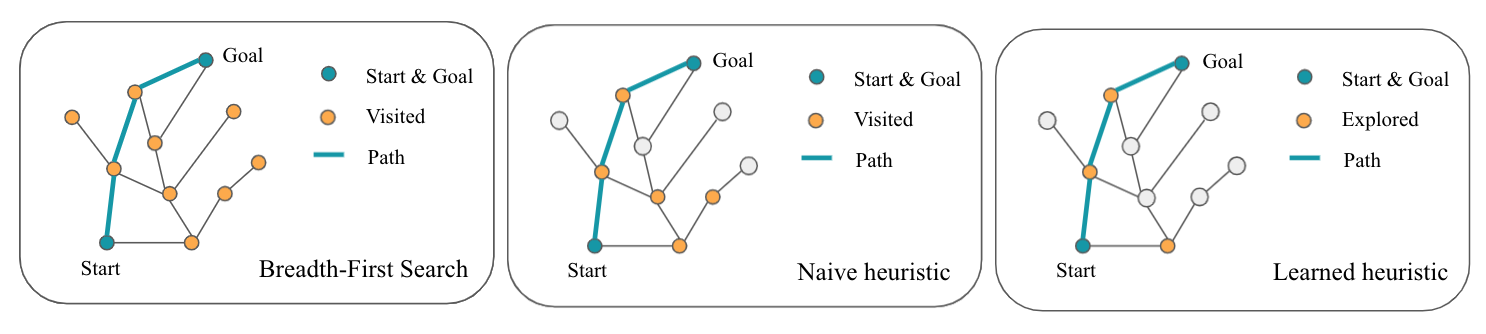
\includegraphics[width=0.9\textwidth]{figures/money_fig.png}
\caption{The goal is to navigate (find a path) from the start to the goal node. While BFS visits many nodes to find a start-to-goal path (left), one can use a heuristic based on the features of the nodes (e.g., Euclidean distance) on the graph to reduce the search effort (middle). We propose \alg to learn a tailored search heuristic for a given graph, capable of reducing the number of visited nodes even further by exploiting the inductive biases of the graph (right). }
\label{fig:money-fig}
\end{figure}

The search task can be formulated as a pathfinding problem on a graph, where given a graph, the task is to navigate and find a short feasible path from a start node to a goal node, while in the process visiting as few nodes as possible (Figure~\ref{fig:money-fig}). The most straightforward approach would be to launch a search algorithm such as breadth-first search (BFS) and iteratively expand the graph from the start node until it reaches the goal node. Since BFS does not harness any prior knowledge about the graph, it usually visits many nodes before reaching the goal, which is expensive in cases such as robotics where visiting nodes is costly. To visit fewer nodes during the search, one may use domain-specific information about the graph via a \textit{heuristic} function \cite{pearl1984heuristics}, which allows one to define a distance metric on graph nodes to prune directions that seem less promising to explore. Unfortunately, coming up with good search heuristics requires significant domain expertise and manual effort.
%, without straightforward ways to further refine proposed heuristics. 

While there has been significant progress in designing search heuristics, it remains a challenging problem. Classical approaches \cite{khalidi2020t, adabala2020multi} tend to hand-design search heuristics, which requires domain knowledge and a lot of trial and error. To alleviate this problem, there has been significant development in general-purpose search heuristics based on trading-off greedy expansions and novelty-based exploration \cite{xie2012planning, xie2014adding, lipovetzky2017best, teichteil2021boundary} or search problem simplifications \cite{bonet2001planning, zhu2003landmark, richter2010lama}. These approaches alleviate some of the common pitfalls of goal-directed heuristics, but we demonstrate that if possible, it is useful to learn domain-specific heuristics that can better exploit problem structure.

On the other hand, learning-based methods face a set of different challenges. Firstly, the data distribution is not i.i.d., as newly encountered graph nodes depend on past heuristic values, which means that supervised learning-based methods are not directly applicable. Secondly, heuristics should run fast, with ideally constant time complexity. Otherwise, the overall asymptotic time complexity of the search procedure could be increased. Finally, as the environment (search graph) sizes increase, reinforcement learning-based heuristic learning approaches tend to perform poorly \cite{bhardwaj2017learning}. State-of-the-art imitation learning-based methods can learn useful search heuristics \cite{bhardwaj2017learning}; however, these methods still rely on feature-engineering for a specific domain and do not generally guarantee a constant time complexity with respect to graph sizes.


\begin{figure}[h]
\centering
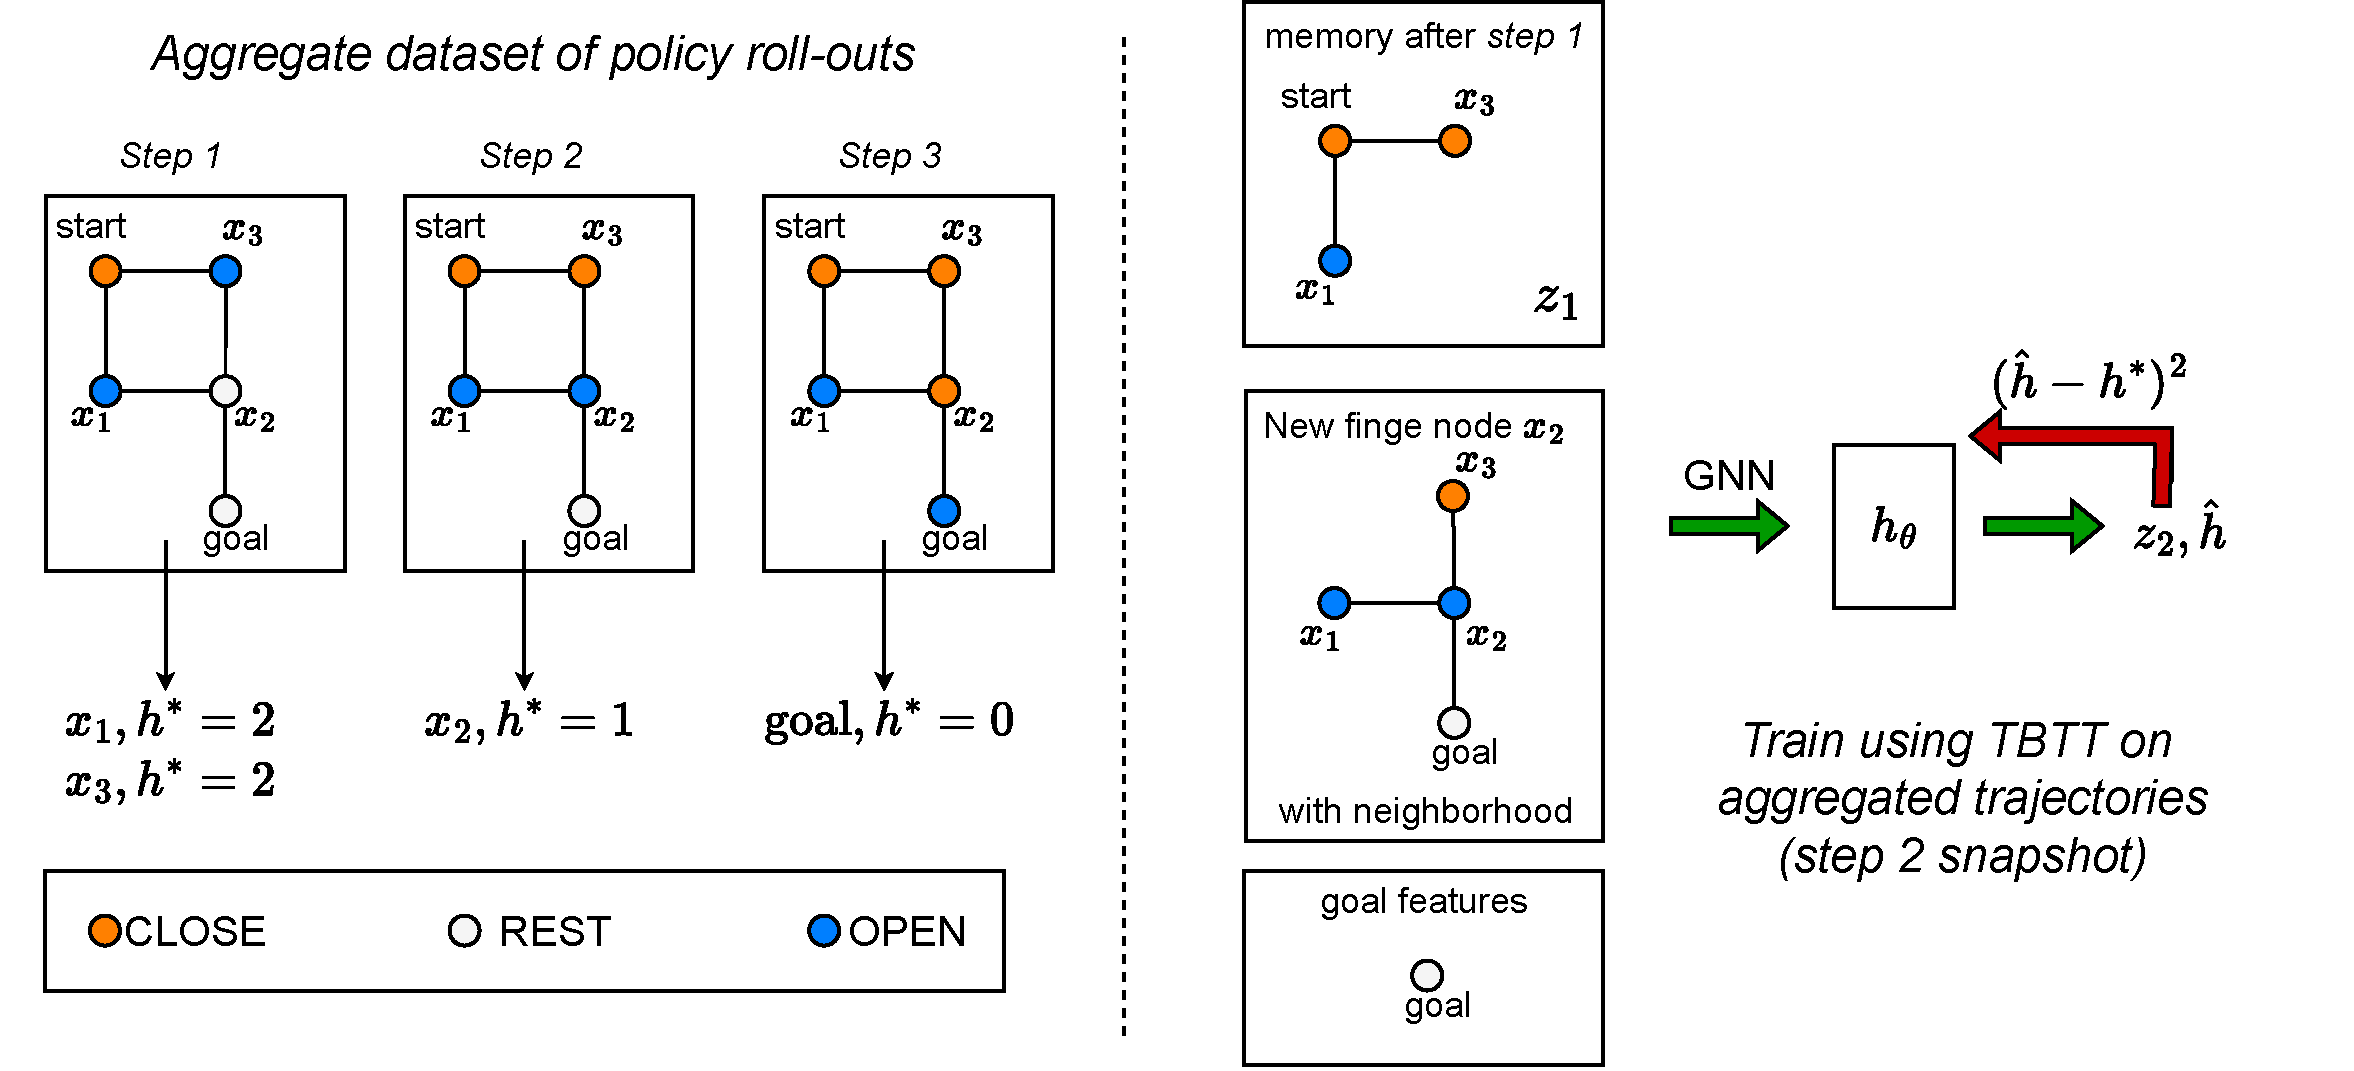
\includegraphics[width=0.9\textwidth]{figures/method_figure2.pdf}
\caption{Main components of \alg: On the left, using a greedy mixture policy induced by the current version of our parameterized heuristic $h_\theta$ and an oracle heuristic $h^*$ (i.e., a heuristic that correctly determines distances between nodes), we roll-out a search trajectory from the start node to the goal node. Each trajectory step contains a set of newly added fringe nodes with bounded random subsets of their 1-hop neighborhoods and their oracle ($h^*$) distances to the goal node. Trajectories are aggregated throughout the training procedure. On the right, we use truncated backpropagation through time on each collected trajectory to train $h_\theta$, where $\hat{h}$ is the predicted distance between $x_2$ and $x_g$, and $z_2$ is the updated state of the memory. Here, the memory captures the embedding of the graph visited so far.}
\label{fig:approach-high-level}
\end{figure}

%\jure{Here we say ``memory'', can we continue the sentence to explain what memory is. Something like: , which captures the graph visited so far.} \update{Added a short sentence at the end}
%\jure{Questions:\\
%-- what is "aggregate dataset"? So far we just explained that there is a graph, a start and a goal node. We need to explain what "aggregate dataset" is or change the label.\\
%-- can we use the concepts introduce in the main text in this figure as well.\\
%-- why do we label $x_{end}$? shouldn't we call it $x_{g}$. Let's use consistent terminology. Also $d_gt$ can we define it.\\
%-- Basically, if we use symbols in the figure, let's define them in the caption.}

%We formulate finding search heuristics as an optimization process, allowing practitioners to quickly find useful search heuristics. We illustrate this concept in Figure \ref{fig:money-fig}.


In this paper, we propose \textit{Path Heuristic with Imitation Learning} (\alg), a framework that extends the recent imitation learning-based heuristic search paradigm with a learnable \textit{explored graph memory}. This means that \alg learns a representation that allows it to capture the structure of the so far explored graph, so that it can then better select what node to explore next (Figure \ref{fig:approach-high-level}).  We train our approach to predict the node-to-goal distances ($h^{*}$ in Figure \ref{fig:approach-high-level}) of graph nodes during search. To train our memory module, which captures the explored graph, we use truncated backpropagation through time (TBTT) \cite{sutskever2013training}, where we utilize ground-truth node-to-goal distances as a supervision signal at each search step. Our TBTT procedure is embedded within an adaptation of the AggreVaTe imitation learning algorithm \cite{ross2014reinforcement}. \alg also includes a \textit{specialized graph neural network architecture}, which allows us to apply \alg to diverse graphs from different domains.

%\jure{Here we introduce many concepts: like ``explored graph'', ``memory module'', ``TBTT'', ``cost-to-go'', ... Can we please make sure to use these concepts in Fig 2 (have some part of the figure labeled using these labels.}

%Figure \ref{fig:approach-high-level} presents the high-level idea of our approach. 

We evaluate \alg on standard benchmark heuristic learning datasets (Section \ref{sec:experiments-grids}), diverse graph-based datasets from different domains (Section \ref{sec:experiments-diversity}), and practical UAV flight use cases (Section \ref{sec:experiments-drone}). Experiments demonstrate that \alg outperforms state-of-the-art heuristic learning methods up to $4 \times$. Further, \alg performs within $4.9 \%$ of an oracle in indoor drone planning scenarios, which is up to a $21.5 \%$ reduction compared with commonly used approaches. In practice, our contributions enable practitioners to quickly extract useful search heuristics from their graph datasets without any hand-engineering.
\section{Preliminaries}
\label{sec:prelims}
\xhdr{Graph search} Suppose that we are given an unweighted connected graph $\mathcal{G} = (\VS, \mathcal{E})$, where $\VS$ is a set of nodes, and $\mathcal{E}$ a corresponding set of edges. Further suppose that each node $i \in \VS$ has corresponding features $x_i \in \mathbb{R}^{D_v}$, and each edge $(i, j) \in \mathcal{E}$ has features $e_{ij} \in \mathbb{R}^{D_e}$. Assume that we are also given a start node $v_s \in \VS$ and a goal node $v_g \in \VS$. At any stage of our search algorithm, we can partition the nodes of our graph into three sets as $\VS = \text{CLOSE} \cup \text{OPEN} \cup \text{REST}$, where CLOSE are the nodes already explored,  $\text{OPEN}$ are candidate nodes for exploration (i.e., all nodes connected to any node in CLOSE, but not yet in CLOSE), and $\text{REST}$ is the rest of the graph. Each \textit{expansion} moves a node from $\text{OPEN}$ to CLOSE, and adds the neighbors of the given node from $\text{REST}$ to $\text{OPEN}$. We call the set of newly added fringe nodes $\VS_{new}$ at each search step.  At the start of the search procedure, $\text{CLOSE} = \{v_s\}$ and we expand the nodes until $v_g$ is encountered (i.e., until $v_g \in \text{CLOSE}$).

\xhdr{Greedy best-first search} We can perform \textit{greedy best-first search} using a greedy fringe expansion policy, such that we always expand the node $v \in \text{OPEN}$ that minimizes $h(v, v_g)$. Here, $h : \VS \times \VS \longrightarrow \mathbb{R}$ is a tailored heuristic function for a given use case. In our work, we are interested in learning a function $h$ that predicts shortest path lengths, this way minimizing $|\text{CLOSE}|$ in a \textit{greedy best-first search} regime.

%\update{Best-first should be clearer now - also organized this section a bit more}


%jure{We never define what a clairvoyant oracle is. Isn't oracle already optimal/supernatural/} \update{We decide to just use oracle for symbol brevity and it's easier to understand.}
\xhdr{Imitation of perfect heuristics} Partially observable Markov decision processes (POMDPs) are a suitable framework to describe the problem of learning search heuristics~\cite{bhardwaj2017learning}. We can have $s = (\text{CLOSE}, \text{OPEN}, \text{REST})$ as our state, an action $a \in \mathcal{A}$ corresponds to moving a node from $\text{OPEN}$ to CLOSE, and the observations $o \in \mathcal{O}$ are the features of newly included nodes in $\text{OPEN}$. Note that one could consider an MDP framework to learn heuristics, but the time complexity of operating on the whole state is in most cases prohibitive. We also define a history $\psi \in \Psi$ as a sequence of observations $\psi = o_1, o_2, o_3, ...$. Our work leverages the observation that using a heuristic function during greedy best-first search that correctly determines the length of the shortest path between fringe nodes and the goal node will also yield minimal $|\text{CLOSE}|$. For training, we adopt a perfect heuristic $h^{*}$, similar to \cite{bhardwaj2017learning}, which has full information about $s$ during search. Such oracle can provide ground-truth distances $h^{*}(s, v, v_g)$, where $v \in \text{OPEN}$. To conclude, we define a \textit{greedy best-first search policy} $\pi_{\theta}$ that uses a parameterized heuristic $h_{\theta}$ to expand nodes from $\text{OPEN}$ with minimal heuristic values. One could also directly use a POMDP solver for the above-described problem, but this approach is usually infeasible due to the dimensionality of the search state \cite{choudhury2017adaptive}.

%\update{Policy defined}

%Consider a partially observable Markov decision process (POMDP) defined by an 8-tuple $(S, A, R, P, \Omega, O, \gamma, \rho_0)$. In this POMDP definition, we have $S$ being a set of valid states, $A$ set of valid actions, $R : S \times A \longrightarrow \mathbb{R}$ the reward function, $P : S \times A \longrightarrow \mathcal{P}(S)$ the transition probability function, $\rho_0$ the initial state distribution, $\gamma \in [0, 1]$ the discount factor, $\Omega$ the set of observations, and $O : S \times A \longrightarrow \mathcal{P}(\Omega)$ a conditional observation probability function. We can also define a history $\psi \in \Psi$ as a sequence of observations $\psi = o_1, o_2, o_3, ...$. In general, our goal is to find an action policy $\pi(\cdot | \psi)$ that maximizes expected discounted rewards under the induced trajectory distribution. 

\section{Related Work}

\xhdr{General purpose heuristic design} There has been significant research in designing general-purpose heuristics for speeding up satisficing planning. The first set of approaches are based on simplifying the search problem for example using landmark heuristics \cite{bonet2001planning, richter2010lama}. The next set of approaches aim to include novelty-based exploration in greedy best-first search \cite{xie2012planning, xie2014adding, lipovetzky2017best, teichteil2021boundary}. The latter set of approaches showed state-of-the-art performance (best-first width search \cite{lipovetzky2017best, teichteil2021boundary}, BFWS) in numerous settings. We show that in domains where data is available, it can be more effective to incorporate a learned heuristic into a greedy best-first search procedure.


\xhdr{Learning heuristic search} There have been numerous previous works that attempt to learn search heuristics: Arfaee \etal \cite{arfaee2011learning} propose to improve heuristics iteratively, Virseda \etal  \cite{us2013learning} learn to combine heuristics to estimate graph node distances, Wilt \etal \cite{wilt2015building} and Garrett \etal \cite{garrett2016learning} propose to learn node rankings, Thayer \etal \cite{thayer2011learning} suggest to infer heuristics during a search, and Kim \etal \cite{KimA20} train a neural network to predict graph node distances. These methods generally do not consider the non-i.i.d. nature of heuristic search. Further, Bhardwaj \etal \cite{bhardwaj2017learning} propose \sail, where heuristic learning is framed as an imitation learning problem with cost-to-go oracles. The \sail heuristic uses hand-designed features tailored for obstacle avoidance, with a linear time-complexity in the number of explored grid nodes found to be colliding with an obstacle. Feature-engineering becomes more difficult as we attempt to learn heuristics on diverse graphs such as ones seen in Section \ref{sec:experiments-diversity}, where we may need expert knowledge. Further, heuristics that do not have a constant time complexity in the size of the graph \cite{bhardwaj2017learning, ariki2019fully, terasawa20203d, yonetani2020path, archetti2021neural} generally scale poorly with graph size and hence have constrained use cases. Recent approaches to learning heuristics include Retro* \cite{chen2020retro} by Chen \etal, where a heuristic is learned in the context of AND-OR search trees for chemical retrosynthetic planning. Our work focuses on a more general graph setting.

There has been significant progress on learning heuristics for NP-hard combinatorial optimization problems \cite{NIPS2017_d9896106, NEURIPS2018_8d3bba74, NEURIPS2020_49f85a9e}. Focusing on solving NP-hard problems allows these approaches to design algorithms that are often non-exact and have a relatively large computational budget. This is not the case for methods that focus on polynomial time search, where learning-based methods are bounded by the determinism and time complexity of classical algorithms such as greedy best-first search.



%Still, these heuristic learning methods, due to their time complexities, are impractical for the application in polynomial-time search problems, on which this work focuses.

%\textbf{\phil generally runs in $\mathcal{O}(1)$ per prediction without requiring any hand-engineering. We provide a comprehensive comparison with \sail in Section \ref{sec:experiments-grids}.}

%recent works by Ariki \etal \cite{ariki2019fully} and Teresawa \etal \cite{terasawa20203d} perform convolutions over full-graphs to infer their heuristic values, which  


\xhdr{Learning general purpose search} 
Learning general search policies is a very well-studied research area with a rich set of developments and applications. These include Monte Carlo Tree Search methods \cite{silver2010monte, guez2018learning}, implicit planning methods \cite{deac2020xlvin, karkus2017qmdp, tamar2016value}, and imagination-based planning approaches \cite{pascanu2017learning, weber2017imagination}. Learning search heuristics can be seen as a special case of \textit{general purpose search}, where the search problem is treated as a partially observable Markov decision process with restricted action evaluation (see Section \ref{sec:approach}), and with models running in $\mathcal{O}(1)$ to remain competitive time-complexity-wise on problems where best-first search performs well. \textit{General purpose search} methods do not take into account the above-mentioned constraints, which motivates the development of tailored approaches for learning heuristics \cite{ bhardwaj2017learning, chen2020retro}.

%\jure{I am not sure what precisely are we trying to say here and how does our method relate/differ from this} \update{The goal here was to answer the question of 'why not just use MCTS or something implicit like VIN'. I tried to rephrase the paragraph so that it is clear. I am also happy to drop this in case you think it is not necessary.}

\xhdr{Imitation learning} Our approach builds on prior work in imitation learning (IL) with cost-to-go oracles. Cost-to-go oracles have been incorporated in the context of IL in methods such as SEARN \cite{daume2009search}, AggreVaTe \cite{ross2014reinforcement}, LOLS \cite{chang2015learning}, AggrevaTeD \cite{sun2017deeply}, DART \cite{laskey2017dart}, and THOR \cite{sun2018truncated}. \sail \cite{bhardwaj2017learning} presents an AggreVaTe-based algorithm for learning heuristic search. We extend \sail by incorporating a recurrent $Q$-like function, in which sense our algorithm more closely resembles AggreVaTeD by Sun \etal \cite{sun2017deeply}. While a recurrent policy can be easily incorporated in AggreVaTeD, we cannot use a policy to evaluate actions. This is due to the fact that we would either have to evaluate all actions in a state, which is computationally infeasible, or we would have to give up on taking actions that are not in the most recent version of the search fringe, which would degrade the performance (see Section \ref{sec:approach}). %RNNs have been previously incorporated in SEARNN by Leblond \etal \cite{searnn} in the context of structured prediction, however we focus on imitation of cost-to-goal oracles. 

%nstead, we propose to use backpropagation through time on the roll-out phase of our algorithm, with cost-to-go supervision on each time step.
\section{Path Heuristic with Imitation Learning}
\label{sec:approach}

%\jure{Notice notation here is using $v_s$, $v_g$, where s is start and t is target. This is not consistent with introduction. Let's fix intro to use the same terminology.}

\xhdr{Training objective} With the aim of minimizing $|\text{CLOSE}|$ after search, our goal is to train a parameterized heuristic function $h_{\theta} : \Psi \times \VS \times \VS \longrightarrow \mathbb{R}$ to predict ground-truth node distances $h^{*}$ and use $h_\theta$ within a greedy best-first policy $\pi_\theta$ at test time.  More specifically, we assume access to a distribution over graphs $P_{\mathcal{G}}$, a start-goal node distribution $P_{v_{sg}}(\cdot \: | \: \mathcal{G})$, and a time horizon $T$. Moreover, we assume a joint state-history distribution $s, \psi \sim P_s(\cdot \: | \: \mathcal{G}, t, \pi_{\theta}, v_s, v_g)$, where $P_s$ represents the probability our search being in state $s$, at time $0 \leq t \leq T$ on graph $\mathcal{G}$ with pathfinding problem $(v_s, v_g)$, with a greedy best-first search policy $\pi_{\theta}$ using heuristic $h_{\theta}$. Hence, our goal can be summarized as minimizing the following objective:

\begin{equation}
    \label{eq:obj}
    \mathcal{L}(\theta) = \mathop{\EX}_{\substack{\mathcal{G} \sim P_{\mathcal{G}}, \\ (v_s, v_g) \sim P_{v_{sg}} \\ t \sim \mathcal{U}(0, ..., T), \\ s, \psi \sim P_s}}\big[\frac{1}{|\text{OPEN}|}\sum_{v \in \text{OPEN}} (h^{*}(s, v, v_g) - h_{\theta}(\psi, v, v_g))^{2} \big]
\end{equation}

Before we describe the algorithm that can be used to minimize $\mathcal{L}$, we rewrite $h_{\theta}$ to include a memory digest component ($z_t$), which represents an embedding of $\psi$ at time step $t$. Hence, $h_\theta$ becomes $h_{\theta} : \mathbb{R}^{d} \times \mathcal{O} \times \VS \times \VS \longrightarrow \mathbb{R}$, where $d$ is the dimensionality of our memory's embedding space. As opposed to previous methods \cite{bhardwaj2017learning}, $z_{t}$ allows us to \textit{automatically extract} relevant features for heuristic computations and concurrently \textit{reduce the computational complexity} of the heuristic function. Further, as shown in \cite{bhardwaj2017learning}, if we would use $h_{\theta}$ to evaluate all actions in a state (i.e., recalculate the heuristic values of all nodes in $\text{OPEN}$), we would need a squared reduction in the number of expanded nodes compared with BFS for \phil to bring performance benefits over BFS, which however may not be possible on all datasets. Hence, we constrain the heuristic only to evaluate new $\text{OPEN}$ nodes which we obtain after moving a node to $\text{CLOSE}$, calling the set of new fringe nodes $\VS_{new}$ after each expansion. In practice, the policy $\pi_{\theta}$  yields an algorithm equivalent to greedy best-first search, with the heuristic function replaced by $h_{\theta}$.

%\jure{This is the first time we define policy $\pi$ and it is unclear that it actually refers to our work PHIL}  \update{Should be clearer now: $\pi_{\theta}$ mentioned at the beginning of approach and in background}

\subsection{Learning algorithm \& architecture}
\label{sec:ila}

\begin{algorithm}[t]
	\caption{\phil --- Sequential Heuristic Training}\label{alg:il_alg}
	Obtain hyperparameters $T$, $\beta_{0}$, $N$, $m$, $t_\tau$;\\
	Initialize $\mathcal{D} \leftarrow \emptyset$, $h_{\theta_{1}}$; \\ \label{lst:line:}
	\For{$i = 1, \ldots, N$}
	{   Sample $\mathcal{G} \sim P_{\mathcal{G}}$; \\
	    Sample $v_s, v_g \sim P_{v_{sg}}$; \\
	    Set $\beta \leftarrow \beta_0^{i}$; \\
        Set mixture policy $\pi_{mix} \leftarrow (1 - \beta) * \pi_{\theta_{i}} + \beta  * \pi^{*}$; \\
	    Collect $m$ trajectories $\tau_{ij}$ as follows; \\
		\For{$j = 1,\ldots,m$}
		{   
			Sample $t \sim \mathcal{U}(0, ..., T - t_{\tau})$;\\
			Roll-in $t$ time steps of $\pi_{\theta_{i}}$ to obtain $z_t$ and new state $s_t = (\text{CLOSE}^{0}, \text{OPEN}^{0}, \text{REST}^{0})$; \\
			Roll-out trajectory $\tau_{ij}$ as follows;\\
			\For{$k = 1,\ldots, t_{\tau}$}
		    {   
    			Update $s_{t + k - 1}$ using $\pi_{mix}$ to get new state $s_{t+k}$ and new fringe state $\text{OPEN}^{k}$; \\
    			Obtain new fringe nodes $\VS_{new} = \text{OPEN}^{k} \setminus \text{OPEN}^{k-1}$; \\
    			Update trajectory $\tau_{ij} \leftarrow \tau_{ij} \cup \{(\VS_{new}, h^{*}(s_{t+k}, \VS_{new}, v_g))\}$; \\
	        }
		    Update dataset $\mathcal{D} \leftarrow \mathcal{D} \cup \{(\tau_{ij}, z_t)\}$ or $\mathcal{D} \cup \{(\tau_{ij}, 0)\}$; \\	
	    }
	    Train $h_{\theta_{i}}$ using TBTT on each $\tau \in \mathcal{D}$ to get $h_{\theta_{i+1}}$;\\  
	}
	\Return{best performing $h_{\theta_{i}}$ on validation};
\end{algorithm}


% Describe algo
\xhdr{Imitation learning algorithm} In Algorithm \ref{alg:il_alg}, we present the pseudo-code of the IL algorithm used to train our heuristic models (Figure \ref{fig:il-proc}). The high-level idea of our algorithm is that we aggregate trajectories of search traces (i.e., sequences of new fringe nodes) and use truncated backpropagation through time to optimize $h_{\theta}$ after each data-collection step. In particular, after sampling a graph $\mathcal{G}$ and a search problem  $v_s, v_g$, we use our greedy learned policy $\pi_\theta$ induced by $h_\theta$ to roll-in for $t \sim \mathcal{U}(0, \dots, T - t_{\tau})$ expansions, where $T$ is the episode time horizon, and $t_\tau$ is the roll-out length. From our roll-in, we obtain a new state $s = (\text{CLOSE}^{0}, \text{OPEN}^{0}, \text{REST}^{0})$, and an initial memory state $z_t$. After our roll-in, we roll-out for $t_{\tau}$ steps using our mixture policy $\pi_{mix}$, which is obtained by probabilistically blending $\pi_\theta$ and the greedy best-first policy induced by the oracle heuristic $\pi^{*}$. In a roll-out, we collect sequences of new fringe nodes, together with their ground-truth distances to the goal $v_g$, given by $h^{*}$.  Once the roll-out is complete, we append the obtained trajectory and the initial state for the following optimization using backpropagation through time. Further analysis on the trade-offs between using rolled-in states $z_t$ or zeroed-out states for training can be found in the supplementary material.

Note that we could also use supervised learning-based approaches to sample a fixed dataset of ($v_s$, $v_g$, $h^{*}(s, v_s, v_g)$) 3-tuples and train a model to predict node distances conditioned on their features. However, our experiments in Section \ref{sec:experiments} demonstrate that ignoring the non-i.i.d. nature of heuristic search negatively impacts model performance, with supervised learning-based methods performing up to $40 \times$ worse.


%\jure{As one is reading this, the question besomese, why not just sample some paths, and learn a MLP or GNN in the IID setting to predict the shortest path distance from current node to goal. It would be good to have a quick paragraph here discussing why this is not a good idea and a forward pointer to experiments/ablations which show that imitation learning gives x\% improvement over IID learning.} \update{Wrote a short paragraph about this.}

\begin{figure}[!htpb]
    \centering
    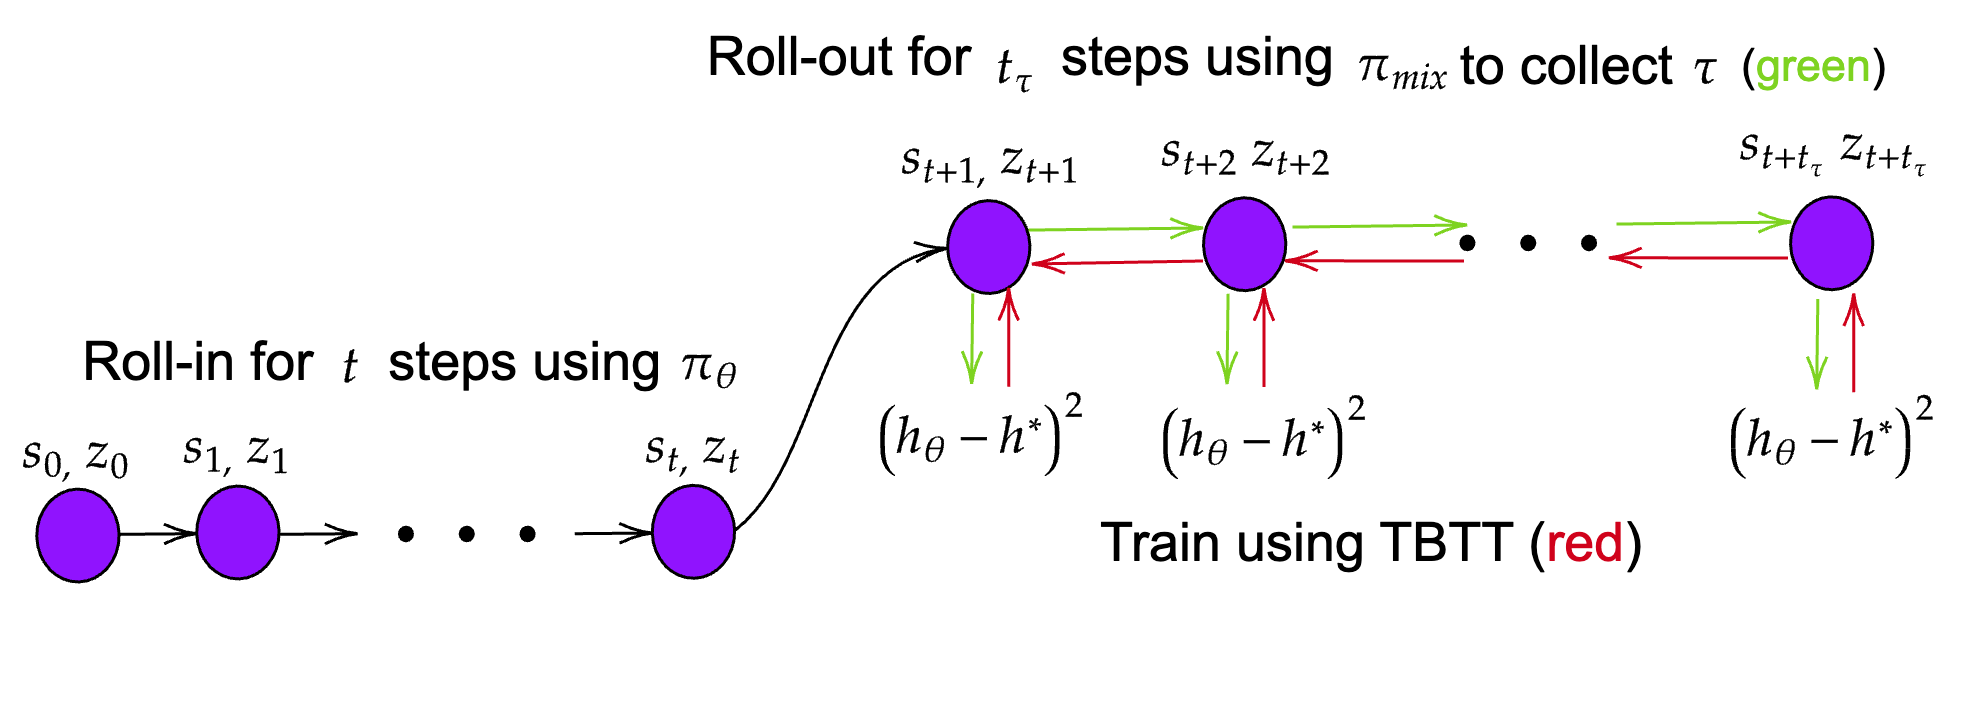
\includegraphics[width=0.9\textwidth]{figures/method_fig.png}
    \caption{This figure demonstrates the core idea behind our IL algorithm. We present the roll-in phase on the left-hand side, where our policy is rolled in for $t$ steps to obtain state $s_t$ and embedding $z_t$. On the right-hand side, we show the trajectory collection and training steps, where we aggregate the trajectory for downstream training (green) and use truncated backpropagation through time on the collected dataset (red).
    }
    \label{fig:il-proc}
    
\end{figure}

\begin{wrapfigure}[12]{R}{0.55\textwidth}
    \begin{algorithm}[H]
    	\caption{Heuristic func. ($h_\theta$) forward pass}\label{alg:htheta_alg}
    	 Obtain $x_i, x_j (j \in \mathcal{N}_i), e_{ij}, x_g$ $z_t$;\\
    	 $x_i \leftarrow f(x_i, x_g, D_{EUC}(x_i, x_g), D_{COS}(x_i, x_g)$);\\
     	 $x_j \leftarrow f(x_j, x_g, D_{EUC}(x_j, x_g), D_{COS}(x_j, x_g)$); \\
    
    	 $g_i \leftarrow \phi(x_i, \mathop{\oplus_{j \in \mathcal{N}_i}} \gamma(x_i, x_j, e_{ij}))$;\\
         $g^{\prime}_i, z_{i, t+1} \leftarrow \textsc{GRU}(g_i, z_t)$;\\
    	 $z_{t+1} \leftarrow \overline{z_{i, t+1}}$;\\ 
    	 $\hat{h}_i \leftarrow \textsc{MLP}(g^{\prime}_i, x_g);$\\
    	\Return{$\hat{h}_i ,z_{t+1}$};\\
    \end{algorithm}
\end{wrapfigure}


\textbf{Recurrent GNN architecture.} In each forward pass, $h_{\theta}$ obtains a set of new fringe nodes $\VS_{new}$, the goal node $v_g$, and the memory $z_t$ at time step $t$. We represent each node in $\VS_{new}$ using its features $x_{i} \in \mathbb{R}^{D_v}$, and likewise the goal node $v_g$ using its features $x_{g} \in \mathbb{R}^{D_v}$. Further, for each $i \in \VS_{new}$, we uniformly sample an $n \in \mathbb{N}_{\geq 0}$ bounded set of nodes present in the 1-hop neighborhood of $i$, calling this set $\mathcal{N}_i$, with $|\mathcal{N}_i| \leq n$. This sampling step produces a set of neighboring node features, where each $j \in \mathcal{N}_i$ has features $x_{j} \in \mathbb{R}^{D_v}$, and corresponding edge features $e_{ij} \in \mathbb{R}^{D_e}$.

%Further, for each $i \in \VS_{new}$, we uniformly sample up to $n \in \mathbb{N}_{\geq 0}$ nodes from the 1-hop neighborhood of $i$. This produces a bounded set of nodes $\mathcal{N}_i$, where $|\mathcal{N}_i| \leq n$, each $j \in \mathcal{N}_i$ has features $x_{j} \in \mathbb{R}^{D_v}$, and corresponding edge features $e_{ij} \in \mathbb{R}^{D_e}$.

%\jure{this header is confusing as for me ''model inference'' means inferring model parameters (and not a forward pass or prediction)}}
%\jure{It would be good to add a sentence here and describe what the goal is and remind people what i,j are and what y adn z are. Basically what are the inputs and what are the outputs} \update{Changed header name, explained what inputs/outputs are}.


\textbf{$h_{\theta}$ forward pass.}  Algorithm \ref{alg:htheta_alg} presents a single forward pass of $h_{\theta}$. The forward pass outputs predicted distances of the new fringe nodes to the goal $\hat{h}_i$, together with an updated memory digest $z_{t+1}$. In Algorithm \ref{alg:htheta_alg}, $f$, $\phi$, $\gamma$, $\textsc{GRU}$\cite{cho-etal-2014-learning}, $\textsc{MLP}$ are each parameterised differentiable functions, with $\phi, \gamma$ representing the \textit{update} and \textit{message} functions~\cite{gilmer2017neural} of a graph neural network, respectively.

In our forward pass, using the function $f$, we first project $x_i, x_j$ into a node embedding space, together with the goal features $x_g$, and their Euclidean ($D_{EUC}$) and cosine distances ($D_{COS}$). After that, using a $1$-layer GNN, we perform a single convolution over each $x_i$ and the corresponding neighborhood $\mathcal{N}_i$, to obtain $g_i$. Our graph convolution processing step allows us to easily incorporate edge features and work with variable sizes of $\mathcal{N}_i$. After the graph convolution, we apply the $\textsc{GRU}$ module over each embedding $g_i$ to obtain hidden states $z_{i, t+1}$, and new embeddings $g^{\prime}_i$. We compute the sample mean of $z_{i, t+1}$ for each node $i \in \VS_{new}$ to obtain a new hidden state $z_{t+1}$, and process $g^{\prime}_i$ with $x_g$ using an $\textsc{MLP}$ to compute the distances between the graph nodes. 

The intuitive explanation for using history embeddings is to address the partial observability of the problem. PHIL does not have access to the full graph because of time complexity concerns. The history embeddings provide a mechanism for keeping track of the belief over the full state of the graph during search. Further, the GNN allows for easily incorporating local neighborhoods and edge features.

\textbf{Permutation invariant $\VS_{new}$ embedding.} There is a trade-off between processing new fringe nodes in batch, as in Algorithm \ref{alg:htheta_alg}, and processing them sequentially. Namely, when we process the nodes in batch, we do not use the in-batch observations to predict batch node values, which means that $z_t$ is slightly outdated. On the other hand, in \phil, batch processing allows us to compute the heuristic values of all $v \in \VS_{new}$ in parallel on a GPU and preserves the memory's permutation invariance with respect to nodes in $\VS_{new}$. That is, because our observations are nodes \& edges of a graph, the respective observation ordering usually does not contain inductive biases useful for predictions, which means that we can apply a permutation invariant operator such as the mean of all new states $z_{i, t+1}$ to obtain an aggregated updated state. This approach provides additional scalability as we can process values in parallel and \phil does not have to infer permutation invariance in $ \VS_{new}$ from data.

\xhdr{Runtime complexity} Since $\forall i \in \VS_{new}: \: |\mathcal{N}_i| \leq n$, Algorithm \ref{alg:htheta_alg} together with neighborhood sampling runs in up to $nc_1 + (n+1)c_2$ operations per each node $i \in \VS_{new}$, which is $\mathcal{O}(1)$ with respect to the size of the graph. Here, $c_1$ is the maximal number of operations associated with evaluating a node, such as performing robot collision checks in dynamically constructed graphs, and $c_2$ is the maximal count of total model operations (e.g., $f$ \& $\gamma$ operations) on the node set $\{i\} \cup \mathcal{N}_i$. Note that for this analysis, we assume that $c_1$ is bounded. In general, we expect to learn a better search heuristic with increasing $n$, but in some use cases, $c_1$ may dominate overall complexity, which means the hyperparameter $n$ is helpful for practitioners to tune trade-offs between constant factors and search effort minimization.
\section{Experiments}
\label{sec:experiments}
In our experiments, we evaluate \phil both on benchmark heuristic learning datasets \cite{bhardwaj2017learning} (Section \ref{sec:experiments-grids}) as well on a diverse set of graph datasets (Section \ref{sec:experiments-diversity}). Finally, we show that \phil can be applied to efficient planning in the context of drone flight (Section \ref{sec:experiments-drone}). Our main goal is to assess how \phil compares to baseline methods in terms of necessary expansions before the goal node is reached.


\subsection{Heuristic search in grids}
\label{sec:experiments-grids}

\begin{wrapfigure}[13]{r}{0.3\textwidth}
  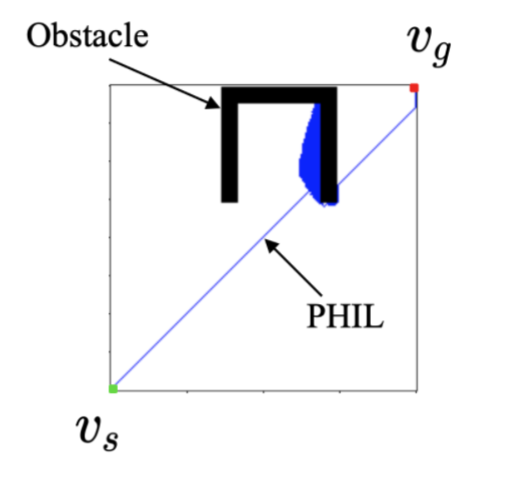
\includegraphics[width=\linewidth]{figures/local_minima.png}
    \caption{Example of \phil escaping local search minima.}
  \label{fig:local-min}
\end{wrapfigure}


In Section \ref{sec:experiments-grids}, we evaluate \phil on $8$, $200 \times 200$ 8-connected grid graph-based datasets by Bhardwaj \etal \cite{bhardwaj2017learning}. These datasets present challenging obstacle configurations for naive greedy planning heuristics, especially when $v_s$ is in the bottom-left of the grid, and $v_g$ in the top-right. Each dataset contains 200 training graphs, 70 validation graphs, and 100 test graphs. Example graphs from each dataset can be found in Table \ref{tab:table-1}.


We train \phil with a hyperparameter configuration of $T = 128$,  $t_{\tau} = 32$, $\beta_{0} = 0.7$, $n = 8$, and using rolled-in $z_t$ states as initial states for training. We use a 3-layer $\textsc{MLP}$ of width 128 with \textit{LeakyReLU} activations, followed by a DeeperGCN \cite{li2020deepergcn} graph convolution with \textit{softmax} aggregation. Our memory’s embedding dimensionality is $64$. The node features are 2D grid coordinates. Note that although using positional representations \cite{you2019position} might be useful for this search problem, it is not scalable as the graph size increases.

\begin{table*}[!htb]
\centering
\caption{The number of expanded graph nodes of \phil with respect to \sail. We can observe that out of all baselines, \sail performs best. \phil outperforms \sail by $58.5 \%$ on average over all datasets, with a maximal search effort reduction of $82.3 \%$ in the \textit{Gaps+Forest} dataset.}
\label{tab:table-1}
\resizebox{\columnwidth}{!}{%

\begin{tabular}{ccccccccccccccc} \toprule
 \textbf{Dataset} & \multicolumn{3}{c}{\textbf{Graph Examples}} & \textbf{\sail} & \textbf{SL} & \textbf{CEM} & \textbf{QL} & \textbf{$h_{euc}$} & \textbf{$h_{man}$} & \textbf{A*} & \textbf{MHA*} & \textbf{BFWS} & \textbf{Neural A*} & \textbf{\phil} \\ \midrule

Alternating gaps    & \frame{
\includegraphics[width=0.6cm, height=0.6cm]{figures/alt_1.png}} &  \frame{
\includegraphics[width=0.6cm, height=0.6cm]{figures/alt_2.png}}  &  \frame{
\includegraphics[width=0.6cm, height=0.6cm]{figures/alt_3.png}}   &0.039	&0.432& 0.042	& 1.000 & 1.000	&1.000	&1.000 & 1.000 & 0.34 &0.546 &\textbf{0.024}\\ 
Single Bugtrap       & \frame{
\includegraphics[width=0.6cm, height=0.6cm]{figures/sb1.png}} & \frame{
\includegraphics[width=0.6cm, height=0.6cm]{figures/sb2.png}}  & \frame{
\includegraphics[width=0.6cm, height=0.6cm]{figures/sb3.png}} 	& 0.158	& 0.214	& 0.057	& 1.000	&0.184	&0.192	&1.000	&0.286 & 0.099 &0.394 & 
\textbf{0.077} \\ 
Shifting gaps       & \frame{
\includegraphics[width=0.6cm, height=0.6cm]{figures/sg1.png}}  & \frame{
\includegraphics[width=0.6cm, height=0.6cm]{figures/sg2.png}}  & \frame{
\includegraphics[width=0.6cm, height=0.6cm]{figures/sg3.png}}  &0.104	&0.464	&1.000	&1.000	&0.506	&0.589	&1.000	&0.804 & 0.206 &0.563 &\textbf{0.027} \\
Forest              & \frame{
\includegraphics[width=0.6cm, height=0.6cm]{figures/f_1.png}}  & \frame{
\includegraphics[width=0.6cm, height=0.6cm]{figures/f2.png}}  &  \frame{
\includegraphics[width=0.6cm, height=0.6cm]{figures/f3.png}}   & 0.036 &0.043	&0.048	&0.121	&0.041	&0.043	&1.000	&0.075 & 0.039  &0.399 & \textbf{0.027}\\
Bugtrap+Forest      & \frame{
\includegraphics[width=0.6cm, height=0.6cm]{figures/bf_1.png}}  & \frame{
\includegraphics[width=0.6cm, height=0.6cm]{figures/bf_2.png}}  &  \frame{
\includegraphics[width=0.6cm, height=0.6cm]{figures/bf_3.png}}  	&0.147	&0.384	&0.182	&1.000	&0.410	&0.337	&1.000	&3.177 & 0.149 &0.651 &\textbf{0.135} \\
Gaps+Forest         &\frame{ 
\includegraphics[width=0.6cm, height=0.6cm]{figures/gf1.png}}  & \frame{
\includegraphics[width=0.6cm, height=0.6cm]{figures/gf2.png}}  & \frame{
\includegraphics[width=0.6cm, height=0.6cm]{figures/gf3.png}}    	&0.221	&1.000	&1.000	&1.000	&1.000	&1.000	&1.000	&1.000 & 0.401 & 0.580 &\textbf{0.039} \\
Mazes               & \frame{
\includegraphics[width=0.6cm, height=0.6cm]{figures/m1.png}}  & \frame{
\includegraphics[width=0.6cm, height=0.6cm]{figures/m2.png}}  & \frame{
\includegraphics[width=0.6cm, height=0.6cm]{figures/m3.png}} 	&0.103	&0.238	&0.479	&0.399	&0.185	&0.171	&1.000	&0.279 & 0.095 &1.000 &\textbf{0.069}\\
Multiple Bugtraps   & \frame{
\includegraphics[width=0.6cm, height=0.6cm]{figures/mb1.png}}  & \frame{
\includegraphics[width=0.6cm, height=0.6cm]{figures/mb2.png}}  & \frame{
\includegraphics[width=0.6cm, height=0.6cm]{figures/mb3.png}} 	&0.479	&0.480	&1.000	&0.835	&0.648	&0.617	&1.000	&0.876 &0.169 &0.331 & \textbf{0.136}  \\ \bottomrule

% Alternating gaps    & \frame{
\includegraphics[width=0.6cm, height=0.6cm]{figures/alt_1.png}} &  \frame{
\includegraphics[width=0.6cm, height=0.6cm]{figures/alt_2.png}}  &  \frame{
\includegraphics[width=0.6cm, height=0.6cm]{figures/alt_3.png}}   &1.000	&11.077	&1.077	&25.641	&25.641	&25.641	&25.641	&25.641 & 8.718 & &\textbf{0.615}\\ 
% Single Bugtrap       & \frame{
\includegraphics[width=0.6cm, height=0.6cm]{figures/sb1.png}} & \frame{
\includegraphics[width=0.6cm, height=0.6cm]{figures/sb2.png}}  & \frame{
\includegraphics[width=0.6cm, height=0.6cm]{figures/sb3.png}} 	&1.000	&1.354	&\textbf{0.361}	&6.329	&1.165	&1.215	&6.329	&1.772 & 0.625 & & 0.544 \\ 
% Shifting gaps       & \frame{
\includegraphics[width=0.6cm, height=0.6cm]{figures/sg1.png}}  & \frame{
\includegraphics[width=0.6cm, height=0.6cm]{figures/sg2.png}}  & \frame{
\includegraphics[width=0.6cm, height=0.6cm]{figures/sg3.png}}      &1.000	&4.462	&9.615	&9.615	&4.865	&5.663	&9.615	&7.731 & 1.982 & &\textbf{0.260} \\
% Forest              & \frame{
\includegraphics[width=0.6cm, height=0.6cm]{figures/f_1.png}}  & \frame{
\includegraphics[width=0.6cm, height=0.6cm]{figures/f2.png}}  &  \frame{
\includegraphics[width=0.6cm, height=0.6cm]{figures/f3.png}}             &1.000	&1.194	&1.333	&3.361	&1.139	&1.194	&27.778	&2.083 & 1.078 & & \textbf{0.778}\\
% Bugtrap+Forest      & \frame{
\includegraphics[width=0.6cm, height=0.6cm]{figures/bf_1.png}}  & \frame{
\includegraphics[width=0.6cm, height=0.6cm]{figures/bf_2.png}}  &  \frame{
\includegraphics[width=0.6cm, height=0.6cm]{figures/bf_3.png}}  	&1.000	&2.612	&1.238	&6.803	&2.789	&2.293	&6.803	&3.177 & 1.011 & &\textbf{0.810} \\
% Gaps+Forest         &\frame{ 
\includegraphics[width=0.6cm, height=0.6cm]{figures/gf1.png}}  & \frame{
\includegraphics[width=0.6cm, height=0.6cm]{figures/gf2.png}}  & \frame{
\includegraphics[width=0.6cm, height=0.6cm]{figures/gf3.png}}    	&1.000	&4.525	&4.525	&4.525	&4.525	&4.525	&4.525	&4.525 & 1.813 & &\textbf{0.213} \\
% Mazes               & \frame{
\includegraphics[width=0.6cm, height=0.6cm]{figures/m1.png}}  & \frame{
\includegraphics[width=0.6cm, height=0.6cm]{figures/m2.png}}  & \frame{
\includegraphics[width=0.6cm, height=0.6cm]{figures/m3.png}} 	&1.000	&2.311	&4.650	&3.874	&1.796	&1.660	&9.709	&2.709 & 0.921 & &\textbf{0.495}\\
% Multiple Bugtraps   & \frame{
\includegraphics[width=0.6cm, height=0.6cm]{figures/mb1.png}}  & \frame{
\includegraphics[width=0.6cm, height=0.6cm]{figures/mb2.png}}  & \frame{
\includegraphics[width=0.6cm, height=0.6cm]{figures/mb3.png}} 	&1.000	&1.002	&2.088	&1.743	&1.353	&1.288	&2.088	&1.829 &0.353 & & \textbf{0.382}  \\ \bottomrule
\end{tabular}
}
\end{table*}

%\jure{Could we add squares/boxes around Graph Examples (as in Fig 4). I think then it will be much clearer that these are same things as in Fig 4).}
%\jure{Caption: Rather than discussing the baselines let's discuss performance and point out interesting observations. For example: ``Out of all baselines \sail performs best, while PHIL performs X\% better than \sail on average.'' Let's say something like this.} \update{boxes and quantified observations added}

\textbf{Discussion.} As we can see in Table \ref{tab:table-1}, \phil outperforms the best baseline (\textit{\sail}) on all datasets, with an average reduction of explored nodes before $v_g$ is found of $58.5 \%$.
%Even with \textit{CEM} performing better than \phil on \textit{Single Bugtrap}, \phil reduces the necessary search effort compared with the best baseline on each dataset by \michal{$40.8 \%$} on average.
Qualitatively, observing Figure \ref{fig:sail-comparison}, we can attribute these results to \phil's ability to \textbf{reduce the redundancy in explored nodes} during a search. Further, \phil is also \textbf{capable of escaping local minima}, which is illustrated in Figure \ref{fig:local-min}. However, note that we occasionally observe failure cases in practice, where \phil gets stuck in a bug trap-like structure.

\xhdr{Runtime \& convergence speed} \phil converges in up to $N = 36$ iterations, with $m = 1, t_\tau = 32$ (i.e., after observing less than $N * t_\tau * max(|\VS_{new}|) \approx 9,216$ shortest path distances, where we take $max(|\VS_{new}|) = 8$ as the maximal size of $\VS_{new}$). According to figures reported in \cite{bhardwaj2017learning}, this is approximately $5\times$ less data than it takes for \sail to converge.
%Although neither the \sail or \phil code-bases were optimized for runtime speed, we found that our implementation of \phil runs about $7 \times$ faster than the publicly available implementation of \sail on the \textit{Gaps+Forest} dataset.


%\jure{Same here, can we quantify performance: PHIL explores X\% less nodes on average than the second best method, Sail} \update{Should be better quantified \& more optimistic}
% \setlength{\framerule}{1pt}%

\begin{figure*}[h!]
    \centering
    \begin{adjustbox}{minipage=\linewidth,scale=0.9}

    \begin{subfigure}[t]{0.45\textwidth}
         \raisebox{-\height}{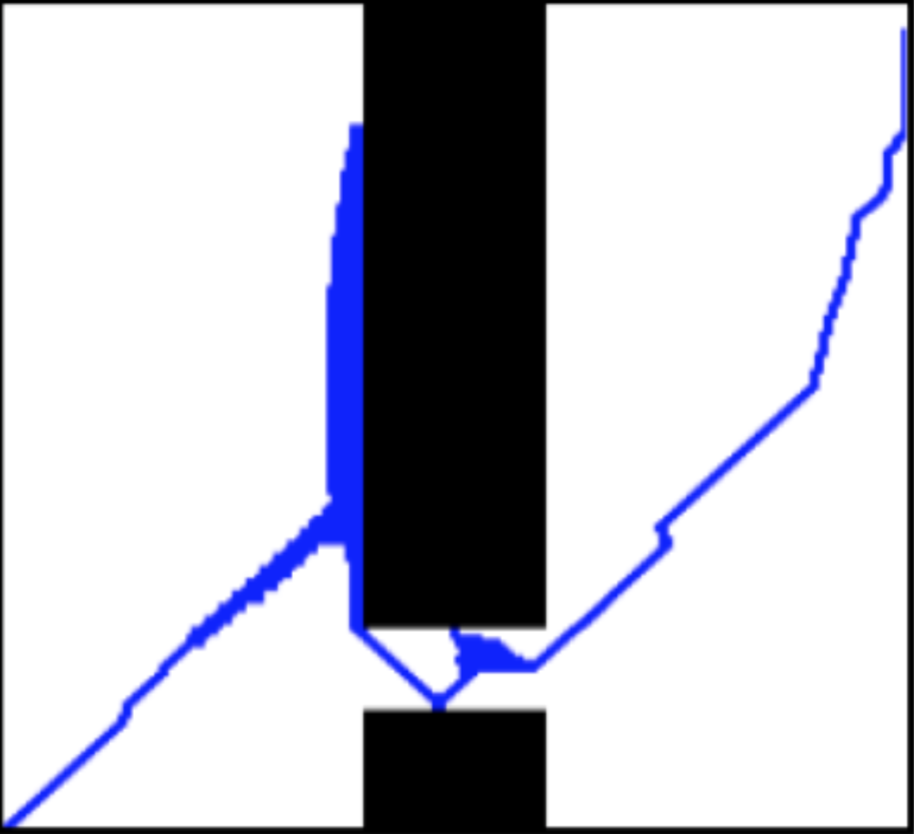
\includegraphics[width=0.49\textwidth,height=0.49\textwidth]{figures/c1_sail.png}}
         \raisebox{-\height}{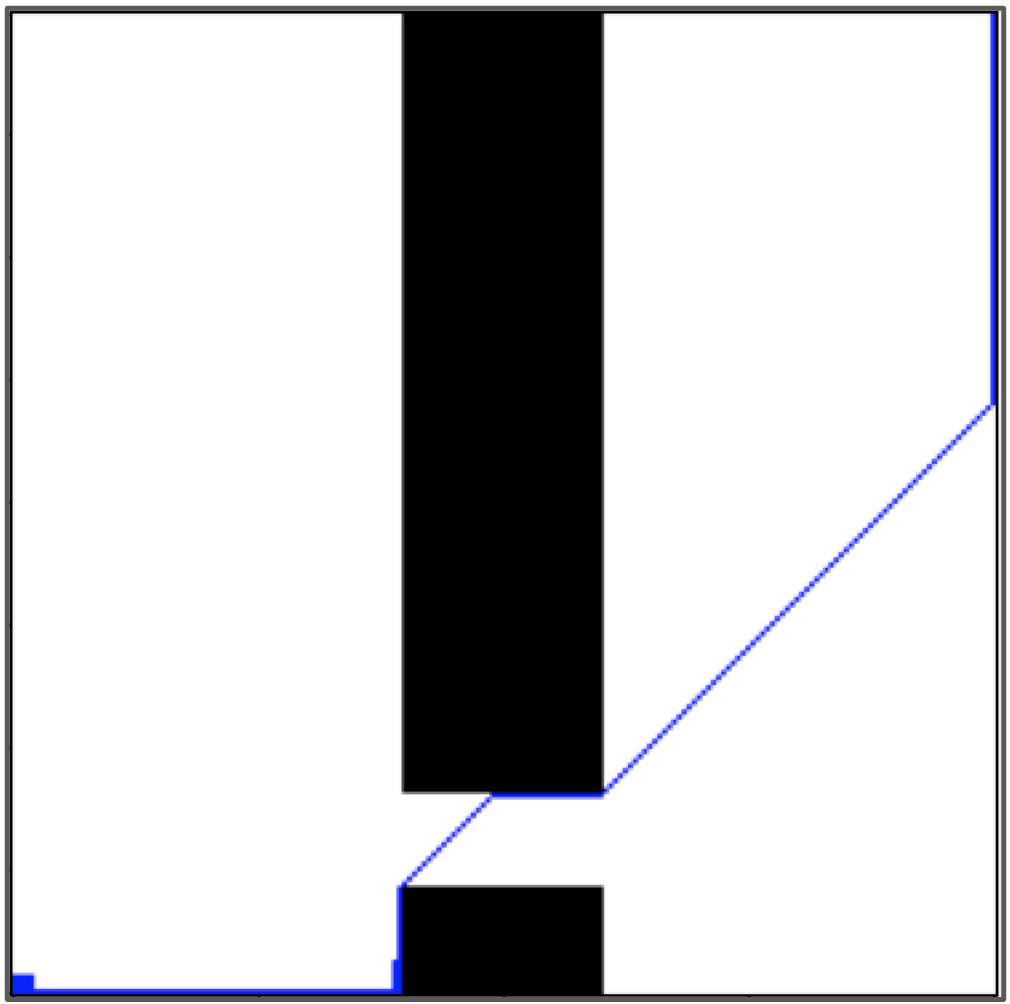
\includegraphics[width=0.49\textwidth,height=0.49\textwidth]{figures/c1.png}}%
         \label{fig:one-a}
    \caption{Shifting gaps (\sail left, \phil right)}
    \end{subfigure}
    \hfill
    \begin{subfigure}[t]{0.45\textwidth}
         \raisebox{-\height}{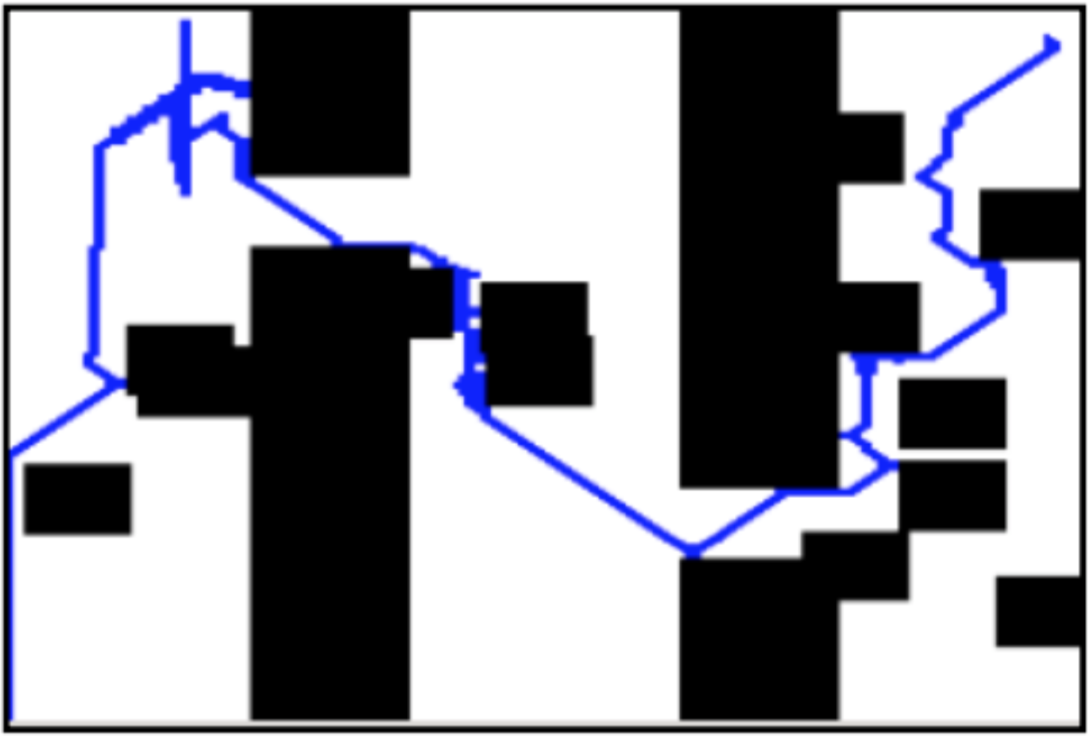
\includegraphics[width=0.49\textwidth,height=0.49\textwidth]{figures/c2_sail.png}}
         \raisebox{-\height}{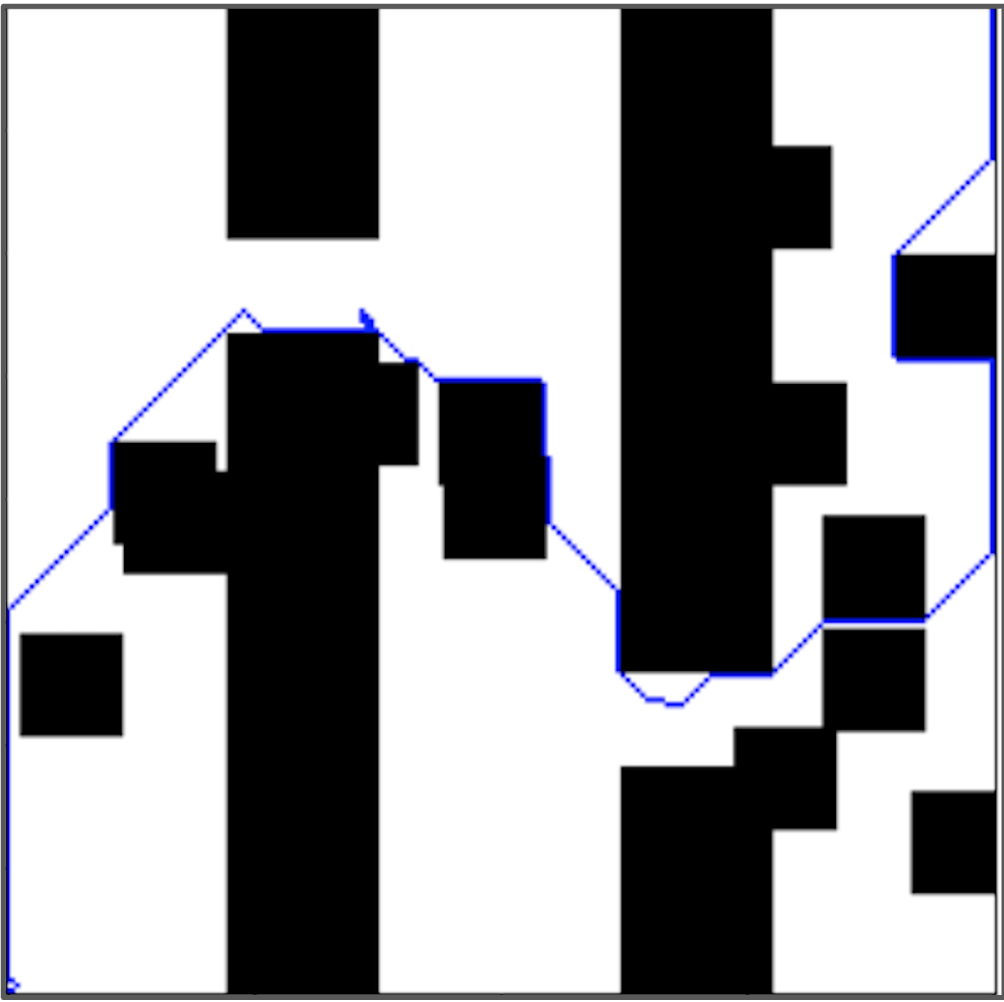
\includegraphics[width=0.49\textwidth,height=0.49\textwidth]{figures/c2.png}}%
    \caption{Gaps+Forest (\sail left, \phil right)}
    \end{subfigure}
    %%%%%%%%%%%%%%%%%%%%%%%%%%%%%%%%%%%%second row
    \begin{subfigure}[t]{0.45\textwidth}
        \raisebox{-\height}{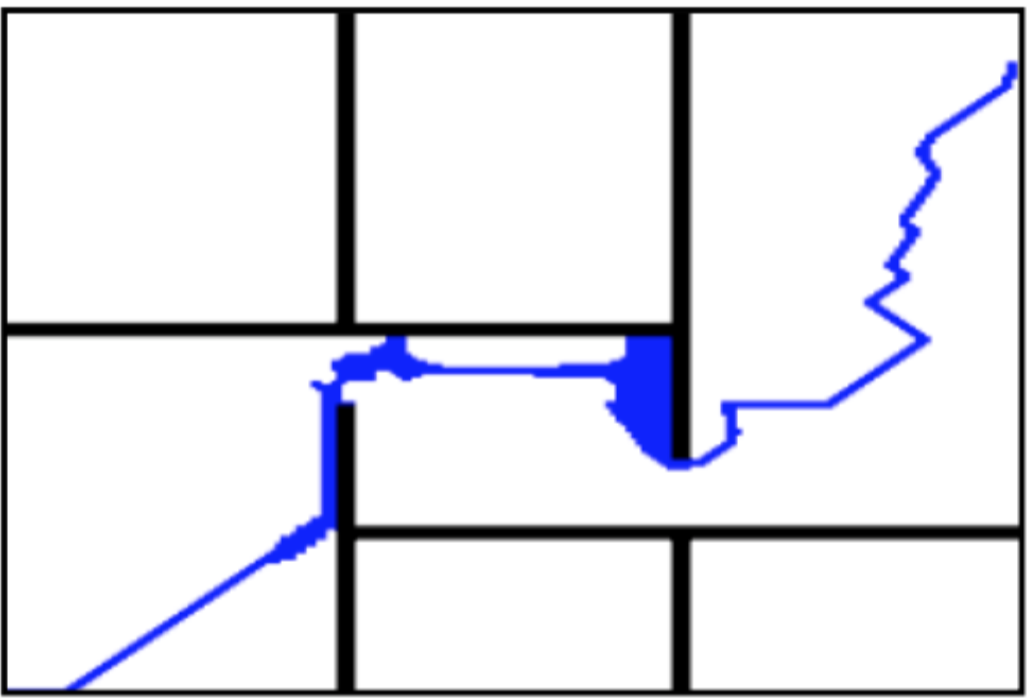
\includegraphics[width=0.49\textwidth,height=0.49\textwidth]{figures/c3_sail.png}}
        \raisebox{-\height}{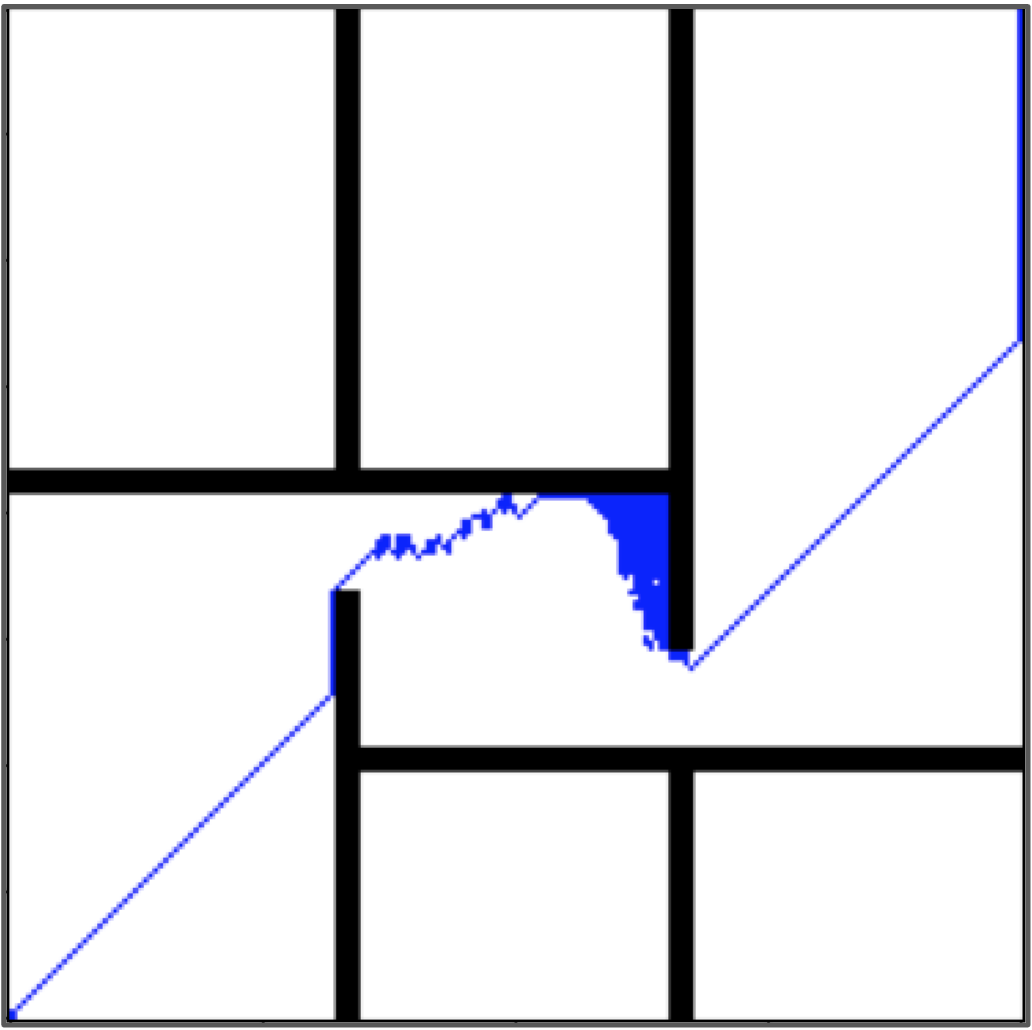
\includegraphics[width=0.49\textwidth,height=0.49\textwidth]{figures/c3.png}}%
    \caption{Mazes (\sail left, \phil right)}
    \end{subfigure}
    \hfill
    \begin{subfigure}[t]{0.45\textwidth}
          \raisebox{-\height}{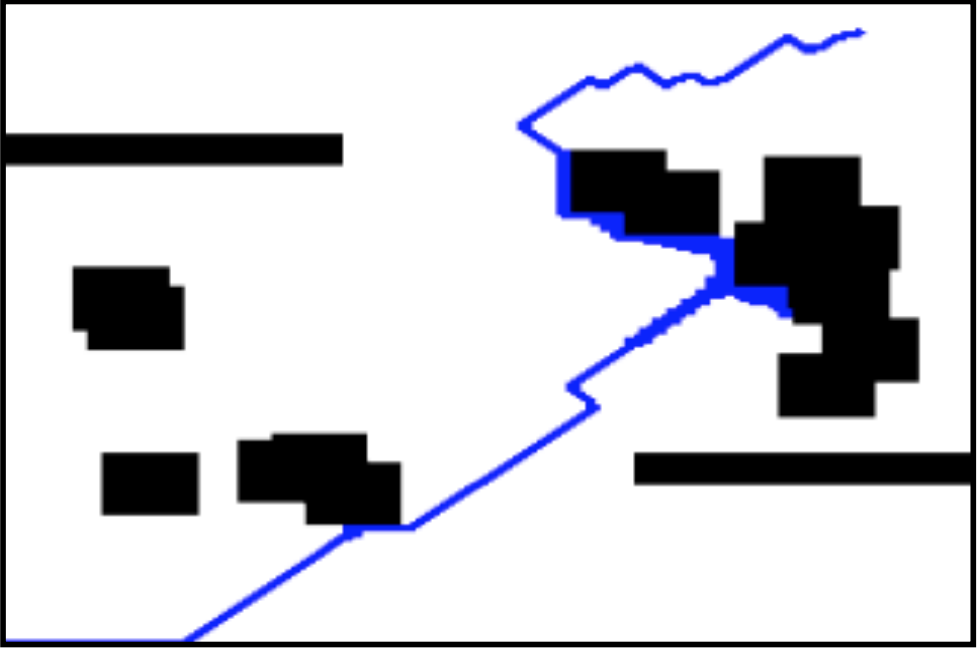
\includegraphics[width=0.49\textwidth,height=0.49\textwidth]{figures/c4_sail.png}}
          \raisebox{-\height}{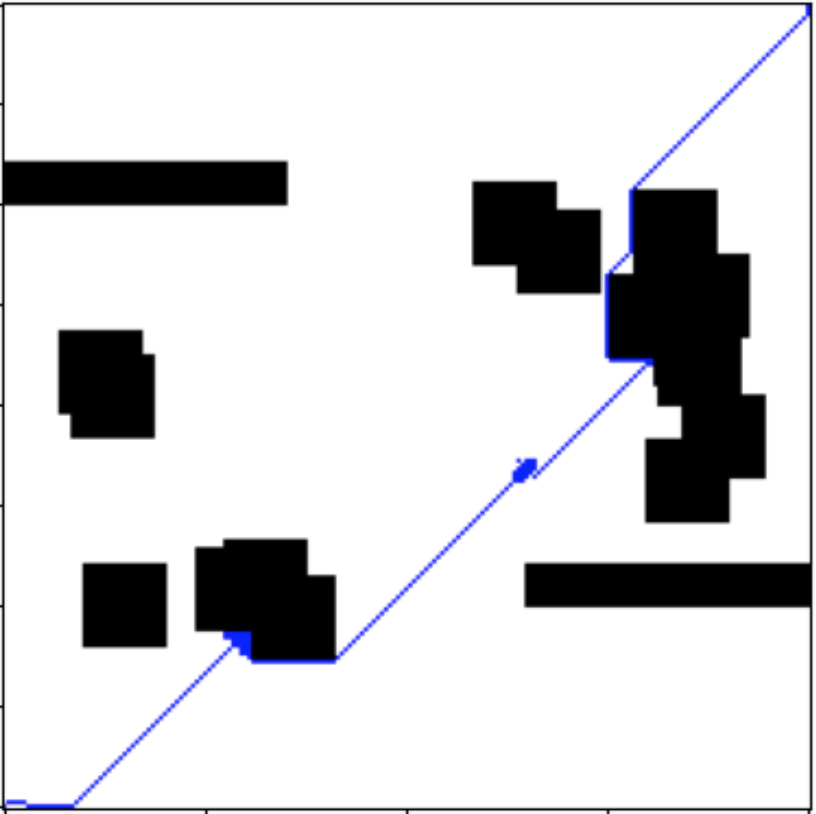
\includegraphics[width=0.49\textwidth,height=0.49\textwidth]{figures/c4.png}}%
    \caption{Forest (\sail left, \phil right)}
    \end{subfigure}
    \end{adjustbox}
    \caption{In each image pair of this figure, we provide a qualitative comparison with the \sail method. In particular, we show comparisons on the \textit{Shifting gaps}, \textit{Gaps+Forest}, \textit{Mazes}, and \textit{Forest} datasets. We can observe that \phil (right) learns the appropriate heuristics for the given dataset and makes fewer redundant expansions than \sail (left).
    %\jure{there seem to be a bug in the figure. I thought that we show the same graph but a different path.} \update{Bug should be fixed}
    } 
    \label{fig:sail-comparison}
\end{figure*}

\subsection{Search in real-life graphs of different structures}
\label{sec:experiments-diversity}

In this experiment, our goal is to demonstrate the general applicability of \phil to various graphs. We train \phil on $4$ different groups of graph datasets: citation networks, biological networks, abstract syntax trees (ASTs), and road networks. We use the same graph for citation networks and road networks for training and evaluation, and we use $100$ random $v_s, v_g$ pairs for testing. In the case of biological networks and ASTs, we usually have train/validation/test splits of $80/10/10$, and in the case of the OGB \cite{hu2020open} datasets, we use the provided splits.


\begin{table*}[!htb]
\centering
\caption{Comparison of \phil with baseline approaches on $4$ groups of datasets: citation networks, biological networks, abstract syntax trees, and road networks. "$-$" denotes being out of a 4-day's training time limit. We can observe that, on average across all datasets, \phil outperforms the best baseline per dataset by $13.4 \%$. Discounting the OGBG datasets, this number becomes $19.5 \%$.}
\label{tab:table-2}
\resizebox{\columnwidth}{!}{

\begin{tabular}{c|c|ccc|ccccccc} 
\toprule
& \textbf{Dataset} &\textbf{$|\mathcal{D}|$} &\textbf{$\bar{|\VS|}$} &\textbf{$\bar{|\mathcal{E}|}$}  & \textbf{SL} &\textbf{A*} &$h_{euc}$ &\textbf{BFS} & \textbf{\sail} & \textbf{BFWS} &\textbf{\phil} \\ \midrule
\multirow{5}{*}{Citation Networks} &Cora (Sen \etal \cite{sen2008collective}) &1 &2,708 &5,429 &2.201	&2.067	&1.000	&4.001 & 0.669 &1.378    &\textbf{0.475} \\ 
&PubMed (Sen \etal \cite{sen2008collective}))   &1 &19,717 &44,338            &2.157 &2.983	&1.000	& 3.853 & 1.196 &  1.000& \textbf{0.745}  \\ 
&CiteSeer (Sen \etal \cite{sen2008collective})) &1 &3,327 &4,732            &1.636 &1.487	&1.000	&2.190 & 1.062     &0.951  &\textbf{0.599}\\
&Coauthor (cs) (Schur \etal \cite{shchur2018pitfalls}) &1 &18,333 &81,894       &1.571	&1.069	&1.000	&2.820 & 1.941 &    1.026 &\textbf{0.835}\\
&Coauthor (physics) (Schur \etal \cite{shchur2018pitfalls}) &1 &34,493 &247,962  &4.076	&1.081	&1.000	&4.523 & $-$ & 1.012 &\textbf{0.964} \\ \midrule
\multirow{4}{*}{Biological Networks} &OGBG-Molhiv  (Hu \etal \cite{hu2020open}) &41,127 &25.5	&27.5  &1.086 &1.065 &\textbf{1.000} & 1.267 & 1.104 & 1.146 & 1.016  \\
&PPI (Zitnik \etal \cite{zitnik2017predicting})         &24 &2,372.67 &34,113.16 &0.772 &0.831 &1.000 &5.618 & 1.746 & 3.941 &\textbf{0.658}\\
&Proteins (Full) (Morris \etal \cite{morris2020tudataset})  &1,113 &39.06 &72.82 &0.995 &0.997 &1.000 &2.645 & 0.891 & 0.966 &\textbf{0.831}\\
&Enzymes (Morris \etal \cite{morris2020tudataset})            &600 &32.63 &62.14 &1.073	&1.007 &1.000 &1.358 & 1.036 & 0.992 &\textbf{0.757}\\ \midrule
\multirow{1}{*}{ASTs} &OGBG-Code2 (Hu \etal \cite{hu2020open}) &452,741 &125.2 &124.2  	&1.196  &1.013	&1.000	&1.267 & 1.029 & \textbf{0.817} & 1.219 \\ \midrule
\multirow{2}{*}{Road Networks} &OSMnx - Modena (Boeing \cite{boeing2017osmnx}) &1 &29,324 &38,309  &2.904 	&3.085	&1.000	&3.493 & 1.182 &0.997&\textbf{0.489}\\ 
&OSMnx - New York (Boeing \cite{boeing2017osmnx}) &1 &54,128 &89,618 & 39.424  &36.529	&1.000	&63.352 & 1.583&1.013 &\textbf{0.962}\\ 
\bottomrule
\end{tabular}
}
\end{table*}


%\jure{Let's add a sentence commenting on performance, let's quantify it.\\
%Also, can we add 2 more columns---size of the graph (nodes, edges).\\
%Call "city networks" "road networks".
%} \update{Added dataset stats and quantified results}

Similarly as in Section \ref{sec:experiments-grids}, our $\textsc{MLP}$ has four layers of width $128$ with \textit{LeakyReLU} activations and we use a DeeperGCN~\cite{li2020deepergcn} graph convolution with \textit{softmax} aggregation. The utilized node and edge features are the provided features in each dataset, except for a few minor modifications. We train an $\textsc{MLP}$ of depth $5$ and width $256$ using supervised learning (SL) for our learning-based baseline method. 

%Our classical baselines are greedy best-first search ($h_{euc}$) and A* with a euclidean distance heuristic on the node features and breadth-first search (BFS). In Table \ref{tab:table-2}, we report the ratio of explored nodes with respect to $h_{euc}$ after search.

\xhdr{Discussion} The results presented in Table \ref{tab:table-2} suggest that \phil can learn superior search heuristics compared with baseline methods, outperforming top baselines per dataset in terms of visited nodes during a search by $13.4 \%$ on average. Two datasets where \phil fell short compared to other baselines are the \textit{OGBG-Molhiv} and \textit{OGBG-Code2} datasets. The \textit{OGBG-Code2} dataset adopts a \textit{project split} \cite{allamanis2019adverse} and OGBG-Mohliv adopts a \textit{scaffold split} \cite{wu2018moleculenet}, both of which ensure that graphs of different structure are present in the training \& test sets. Although \phil improved upon uninformed search (BFS) in the OGB datasets, structural graph consistency is explicitly discouraged in the above-mentioned OGBG splits. Without the OGBG datasets, \phil improves on the top baselines per dataset by $19.5 \%$ on average, and upon the Euclidean node feature heuristic ($h_{euc}$) by $20.4 \%$. Note that we trained \phil up to $N = 60$ iterations, which means that it only encountered a small subset of the pathfinding problems in the single graph setting, which means that \phil had to generalize to learn useful heuristics. Even in Cora, the $|\mathcal{D}| = 1$ dataset with least number of nodes, \phil observed roughly $6,000$ node distances during training, which is less than $0.2 \%$ of total distances in the Cora graph.

%The \textit{OGBG-Molhiv} and \textit{OGBG-Code2} datasets contain a diverse set of molecules (approx. $40, 000$) and code-bases (approx. $400, 000$), respectively. Contrary to the grid datasets from our previous experiments, where both train and test datasets were structurally similar




%\jure{Same here, can we quantify performance: PHIL explores X\% less nodes on average than the second best method.} \update{Should be better quantified}


%\jure{This is interesting but perhaps not too important. We can cut it and use space to make the method description less dense} \xhdr{Road network results} Further, we can observe the difference in the performance of \phil on the \textit{OSMnx - Modena} and \textit{OSMnx - New York} \cite{boeing2017osmnx} networks. The network of New York resembles a regular grid-like graph, where using naive heuristics is close to optimal. On the other hand, Modena presents a more irregular graph structure, where purely distance minimizing expansions are often incorrect. The relative irregularity of Modena is also evidenced by the fact that in the graph of New York, distance minimizing expansions yield on average $|\VS_{seen}|$ only $6\times$ larger than the lengths of shortest paths, while in Modena, this number is approximately $60$. \phil can bring significant upsides to the euclidean heuristic, especially when the euclidean heuristic is far from optimal. We can conclude that the main use-cases of \phil are in applications where the graphs present in the application domain are structurally similar to training datasets, and where feature distance minimizing expansions are not close to optimal.

\subsection{Planning for drone flight}
\label{sec:experiments-drone}

%Suppose that we wish to operate an autonomous UAV in a densely populated indoor area. An essential component of our UAV would be a planning module, which is classically implemented by treating the environment as a dense 3D grid graph and running a pathfinding algorithm such as A*. In practice, due to our UAV's limited onboard computation capabilities \cite{liu2018motion}, node expansion becomes a performance bottleneck, especially as it can include a complex set of collision and regulation compliance checks. We may relax the shortest path requirement and include additional heuristics in our search algorithm to solve this issue. However, coming up with heuristics that minimize search effort is not a trivial task, as these can depend on the structure of the environment, the local regulations, and possibly the geometry of the UAV.


\begin{wrapfigure}[17]{r}{0.4\textwidth}
  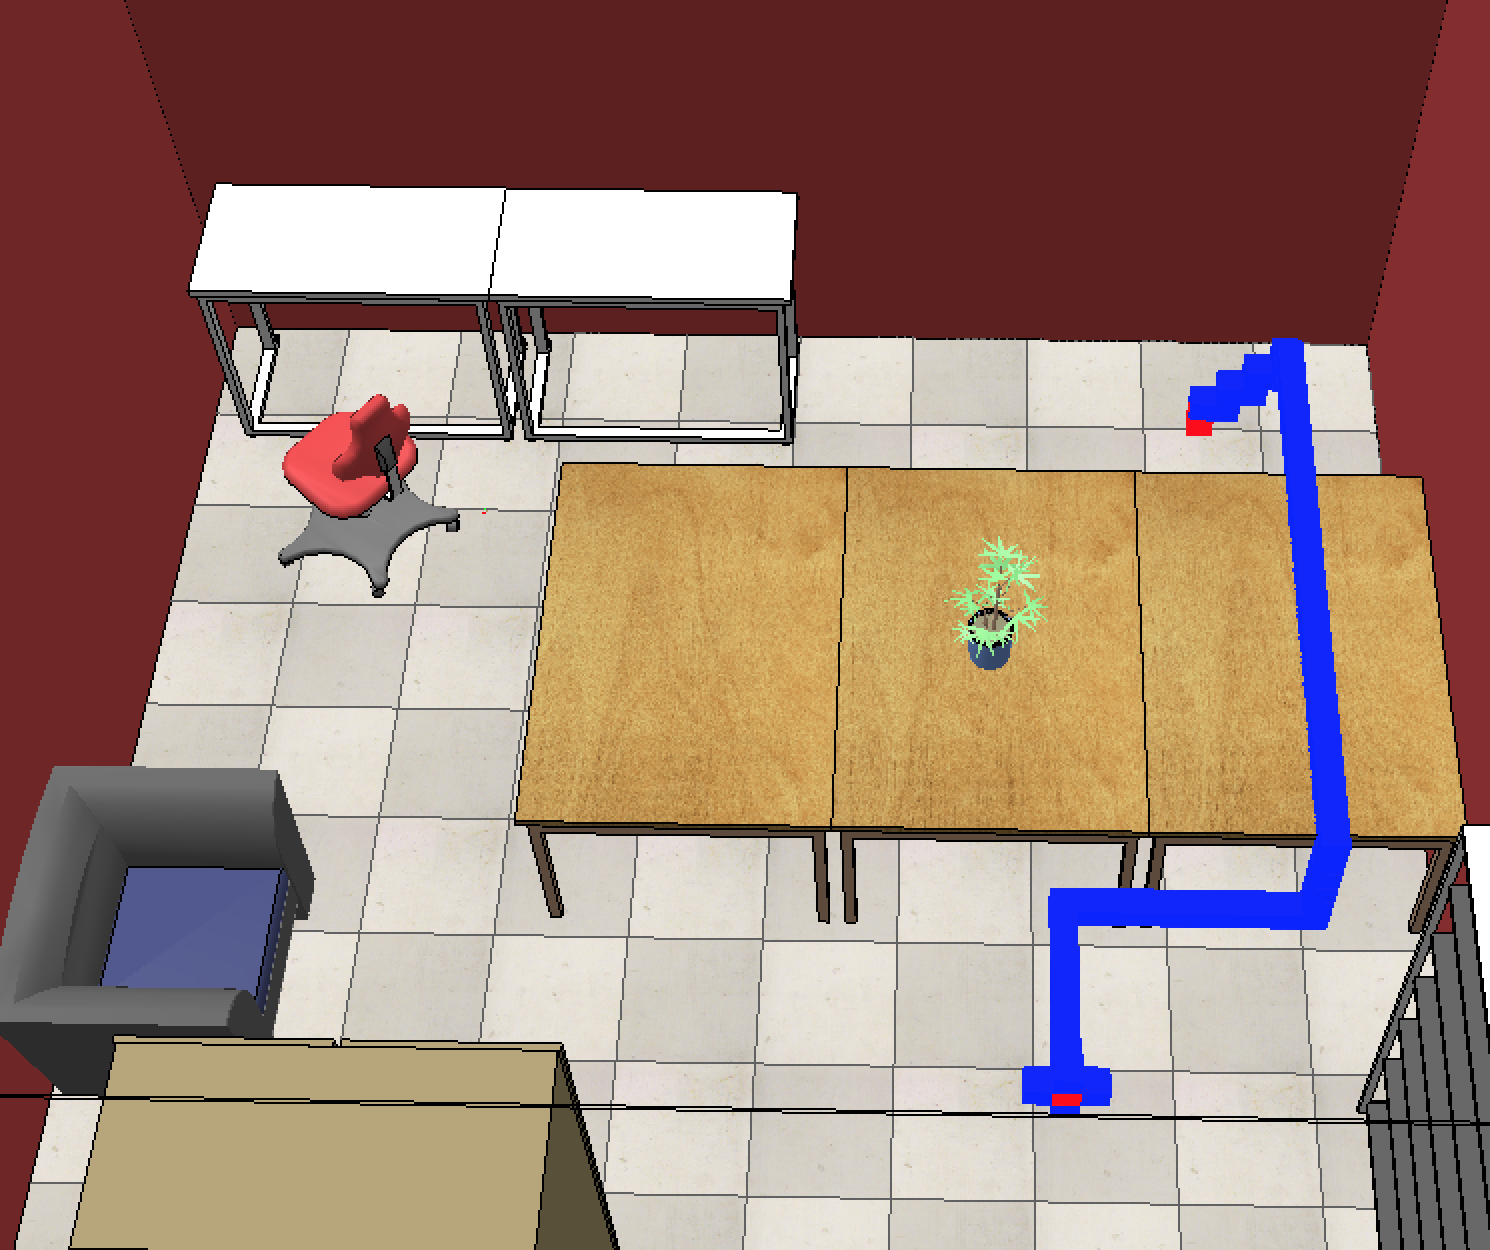
\includegraphics[width=0.9\linewidth]{figures/planned_path.png}
    \caption{This figure illustrates the \textit{room adversarial} environment with an example planning problem (red) and the expanded graph by \phil (blue).}
  \label{fig:room-adv}
\end{wrapfigure}

In our final experiment, we use \phil to plan collision-free paths in a practical drone flight use case within an indoor environment. We built our environment using the CoppeliaSim simulator \cite{coppeliaSim}, and the Ivy framework \cite{lenton2021ivy}. Figure \ref{fig:room-adv}  presents the environment which we refer to as \textit{room adversarial} in Table \ref{tab:table-3}. We discretize the environments into 3D grid graphs of size $50 \times 50 \times 25$, and randomly remove $5$ sub-graphs of size  $5 \times 5 \times 5$ both during training and testing, this way simulating real-life planning scenarios with random obstacles. The hyperparameter configuration and the specific architecture we utilize are equivalent to Section \ref{sec:experiments-grids}, but with $n = 4$. Likewise, the node features are 3D grid coordinates, and the baselines include supervised learning (SL), $h_{euc}$, A*, and BFS, similarly as in Sections \ref{sec:experiments-grids}, \ref{sec:experiments-diversity}. In Table \ref{tab:table-3} we report the ratio of expanded nodes with respect to $h_{euc}$. 

\xhdr{Video demo} We provide a video demonstration of \phil running in \textit{room adversarial}: \url{https://cutt.ly/eniu5ax}.
\begin{table*}[!htb]
\centering
\caption{Results of \phil in the context of planning for indoor UAV flight. \phil outperforms all baselines in both the \textit{room simple} and \textit{room adversarial} environments while remaining close performance-wise to the optimal number of expansions.}
\label{tab:table-3}
\resizebox{0.7\columnwidth}{!}{%

\begin{tabular}{cccccccc|c} \toprule
 \textbf{Dataset}                     & \textbf{SL} &\textbf{A*} & $h_{euc}$ & \textbf{BFS} & \textbf{\sail} & \textbf{BFWS} & \textbf{\phil} & \textbf{Shortest path} \\ \midrule
Room simple   & 1.124 & 76.052  & 1.000 & 291.888 & 0.973 & 1.286 & \textbf{0.785} &0.782                 \\ 
Room adversarial  & 2.022 & 67.215   & 1.000 & 238.768 & 0.944 & 1.583 & \textbf{0.895} & 0.853                  \\ \bottomrule
\end{tabular}
}
\end{table*}

\xhdr{Discussion} As we can observe in Table \ref{tab:table-3}, \phil outperforms all baselines in both environments. Interestingly, \phil expands only approximately $0.3\%$ more nodes in the simple room than least possible and $4.9\%$ more in the adversarial room case. The same figures for the greedy method ($h_{euc}$) are $27.8\%$  and $17.2 \%$, respectively. These results indicate that \phil is capable of learning planning strategies that are close to optimal in both \textit{simple} and \textit{adversarial} graphs, while the performance of naive heuristics degrades.

\subsection{Runtime Analysis}
\label{sec:runtime}
We evaluated the inference runtimes of seven approaches on all datasets in Section~\ref{sec:experiments-grids}. Each approach's runtime was normalized by the number of nodes it visited. The runtime experiments were conducted on a machine with an RTX5000 GPU and an Intel Xeon 5222 CPU.

\begin{figure}[H]
    \centering
    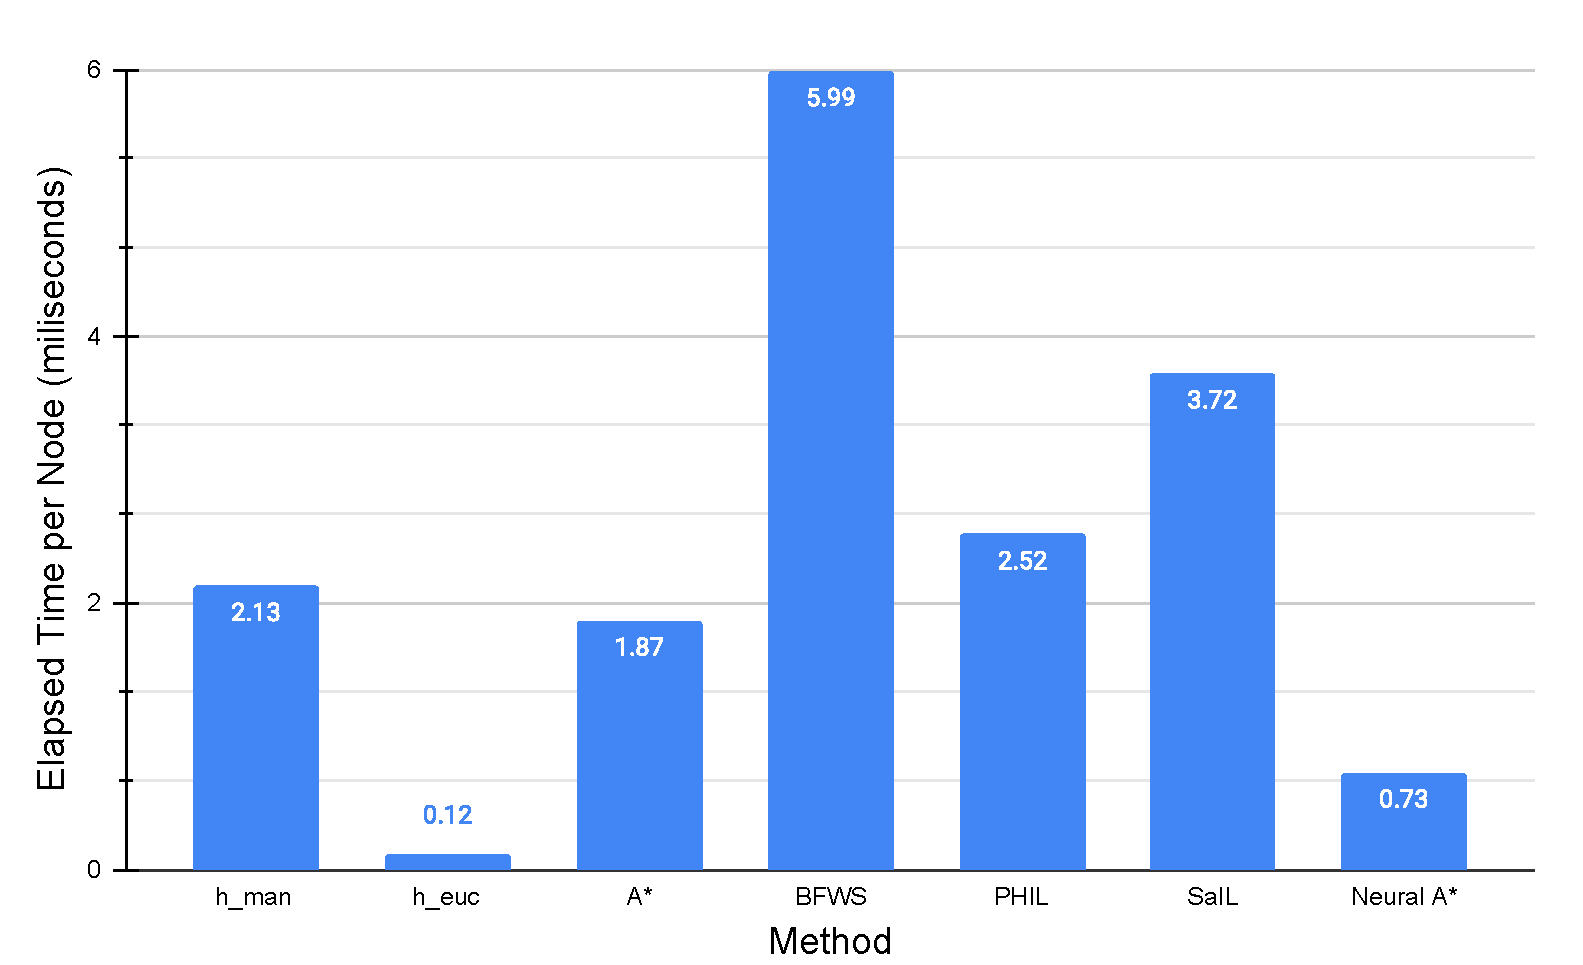
\includegraphics[width=0.9\linewidth]{PHIL/figures/runtime.pdf}
    \caption{Timing experiments on grid search datasets \cite{bhardwaj2017learning}.}
    \label{fig:phil-runtime}
\end{figure}

Figure~\ref{fig:phil-runtime} summarizes the test runtimes of the different approaches. PHIL runs $57.9\%$ faster than BFWS and $32.2\%$ faster than \sail , and not much slower than traditional A* ($34.7\%$) and $h_{man}$ ($18.3\%$). Although Neural A* is $71.0\%$ faster than PHIL due to the fact that it casts the whole search process into matrix operations on images, it cannot be employed in a generic search setting.
\section{Conclusion}

We consider the problem of learning to search for feasible paths in graphs efficiently. We propose a model and a training procedure to learn search heuristics that can be easily deployed across diverse graphs, with tuneable trade-off parameters between constant factors and performance. Our results demonstrate that \phil outperforms current state-of-the-art approaches and can be applied to various graphs with practical use cases.

    \label{chapter:hybrid}

\section{Introduction}
\label{sec:hybrid-intro}


Discovering relations among brain regions toward a specific phenotypic outcome from fMRI signals has been a crucial area in neuroimaging research. Reliable and informative relations help neuroscientists and clinical professionals to better understand brain functions, and thus improve clinical diagnosis and treatments \citep{kucian2008development,kucian2006impaired, li2015putting,li2015toward,satterthwaite2015linked,wang2016efficient}.
However, despite the clear multiplexity of the brain's involvement in cognition \citep{logue2014neural,barrasso2016neurobiological,knauff2010complex,reineberg2022context}, current imaging biomarker detection methods \citep{shen2017using,gao2019combining,li2021braingnn} focus only on the contributing roles of the pairwise connectivity edges. In contrast, most brain functions involve distributed patterns of interactions among multiple regions \citep{semedo2019cortical}. For instance, executive planning requires the appropriate communication of signals across many distinct cortical areas \citep{logue2014neural}. 
These high-order relationships, cannot always be decomposed into pairwise ones \cite{battiston2020networks, battiston2021physics, bick2023higher}, thus allowing them to capture information beyond the reach of pairwise ones \cite{do2020structural}. Consequently, relying solely on pairwise connectivity, without accounting for the brain's complex high-order structure, may result in inconsistent findings and low predictive performance across studies. 
Although recently there have been a few works \citep{zu2016identifying,xiao2019multi,li2022construction} working on discovering the high-order relationships of brain regions, they are unable to effectively extract meaningful patterns. This is because these methods usually first identify some candidates of high-order relationships and then perform feature selection. The candidates are obtained by enumerating only a small portion of all possible relations, or by clustering methods that are unrelated to the target. As a result, most informative high-order relations are likely excluded at the first stage. This inspires us to solve the problem in an end-to-end manner through a more expressive model and a more appropriate objective.

%1) the discovering process of high-order relationships is not guided by cognitive targets; 2) the weak expressiveness of traditional machine learning methods (e.g. lasso regression) hinders the accurate modeling of brain region interactions \citep{cao2022brain,richards2019deep}.

In this paper, we aim to identify high-order relationships that are informative towards a phenotypic outcome, such as a cognition score. However, unlike pairwise relations, the number of possible high-order relations is exponential. To identify the most informative ones from the exponential space, we propose our objective: \textit{maximally informative and minimally redundant} (MIMR). That is to say, we maximize the information contained in the high-order relationships towards a neurological outcome (\textit{informativeness}) while diminishing the participation of unrelated brain regions (\textit{redundant}).
% \todo{more citations in this paragraph to justify the principle would be awesome. We could even move some of the citations from previous paragraphs here if relevant.} 
Such a criterion, on the one hand, ensures the predictive performance of these high-order relationships; on the other hand, it endows the model with the capacity to identify more succinct and interpretable structures \citep{yu2020graph,miao2022interpretable,miao2022interpretable2,chen2023tempme}. A formal definition of the MIMR criterion could be found in Equation \ref{equ:ib2} from an information bottleneck point of view.

\begin{figure}
    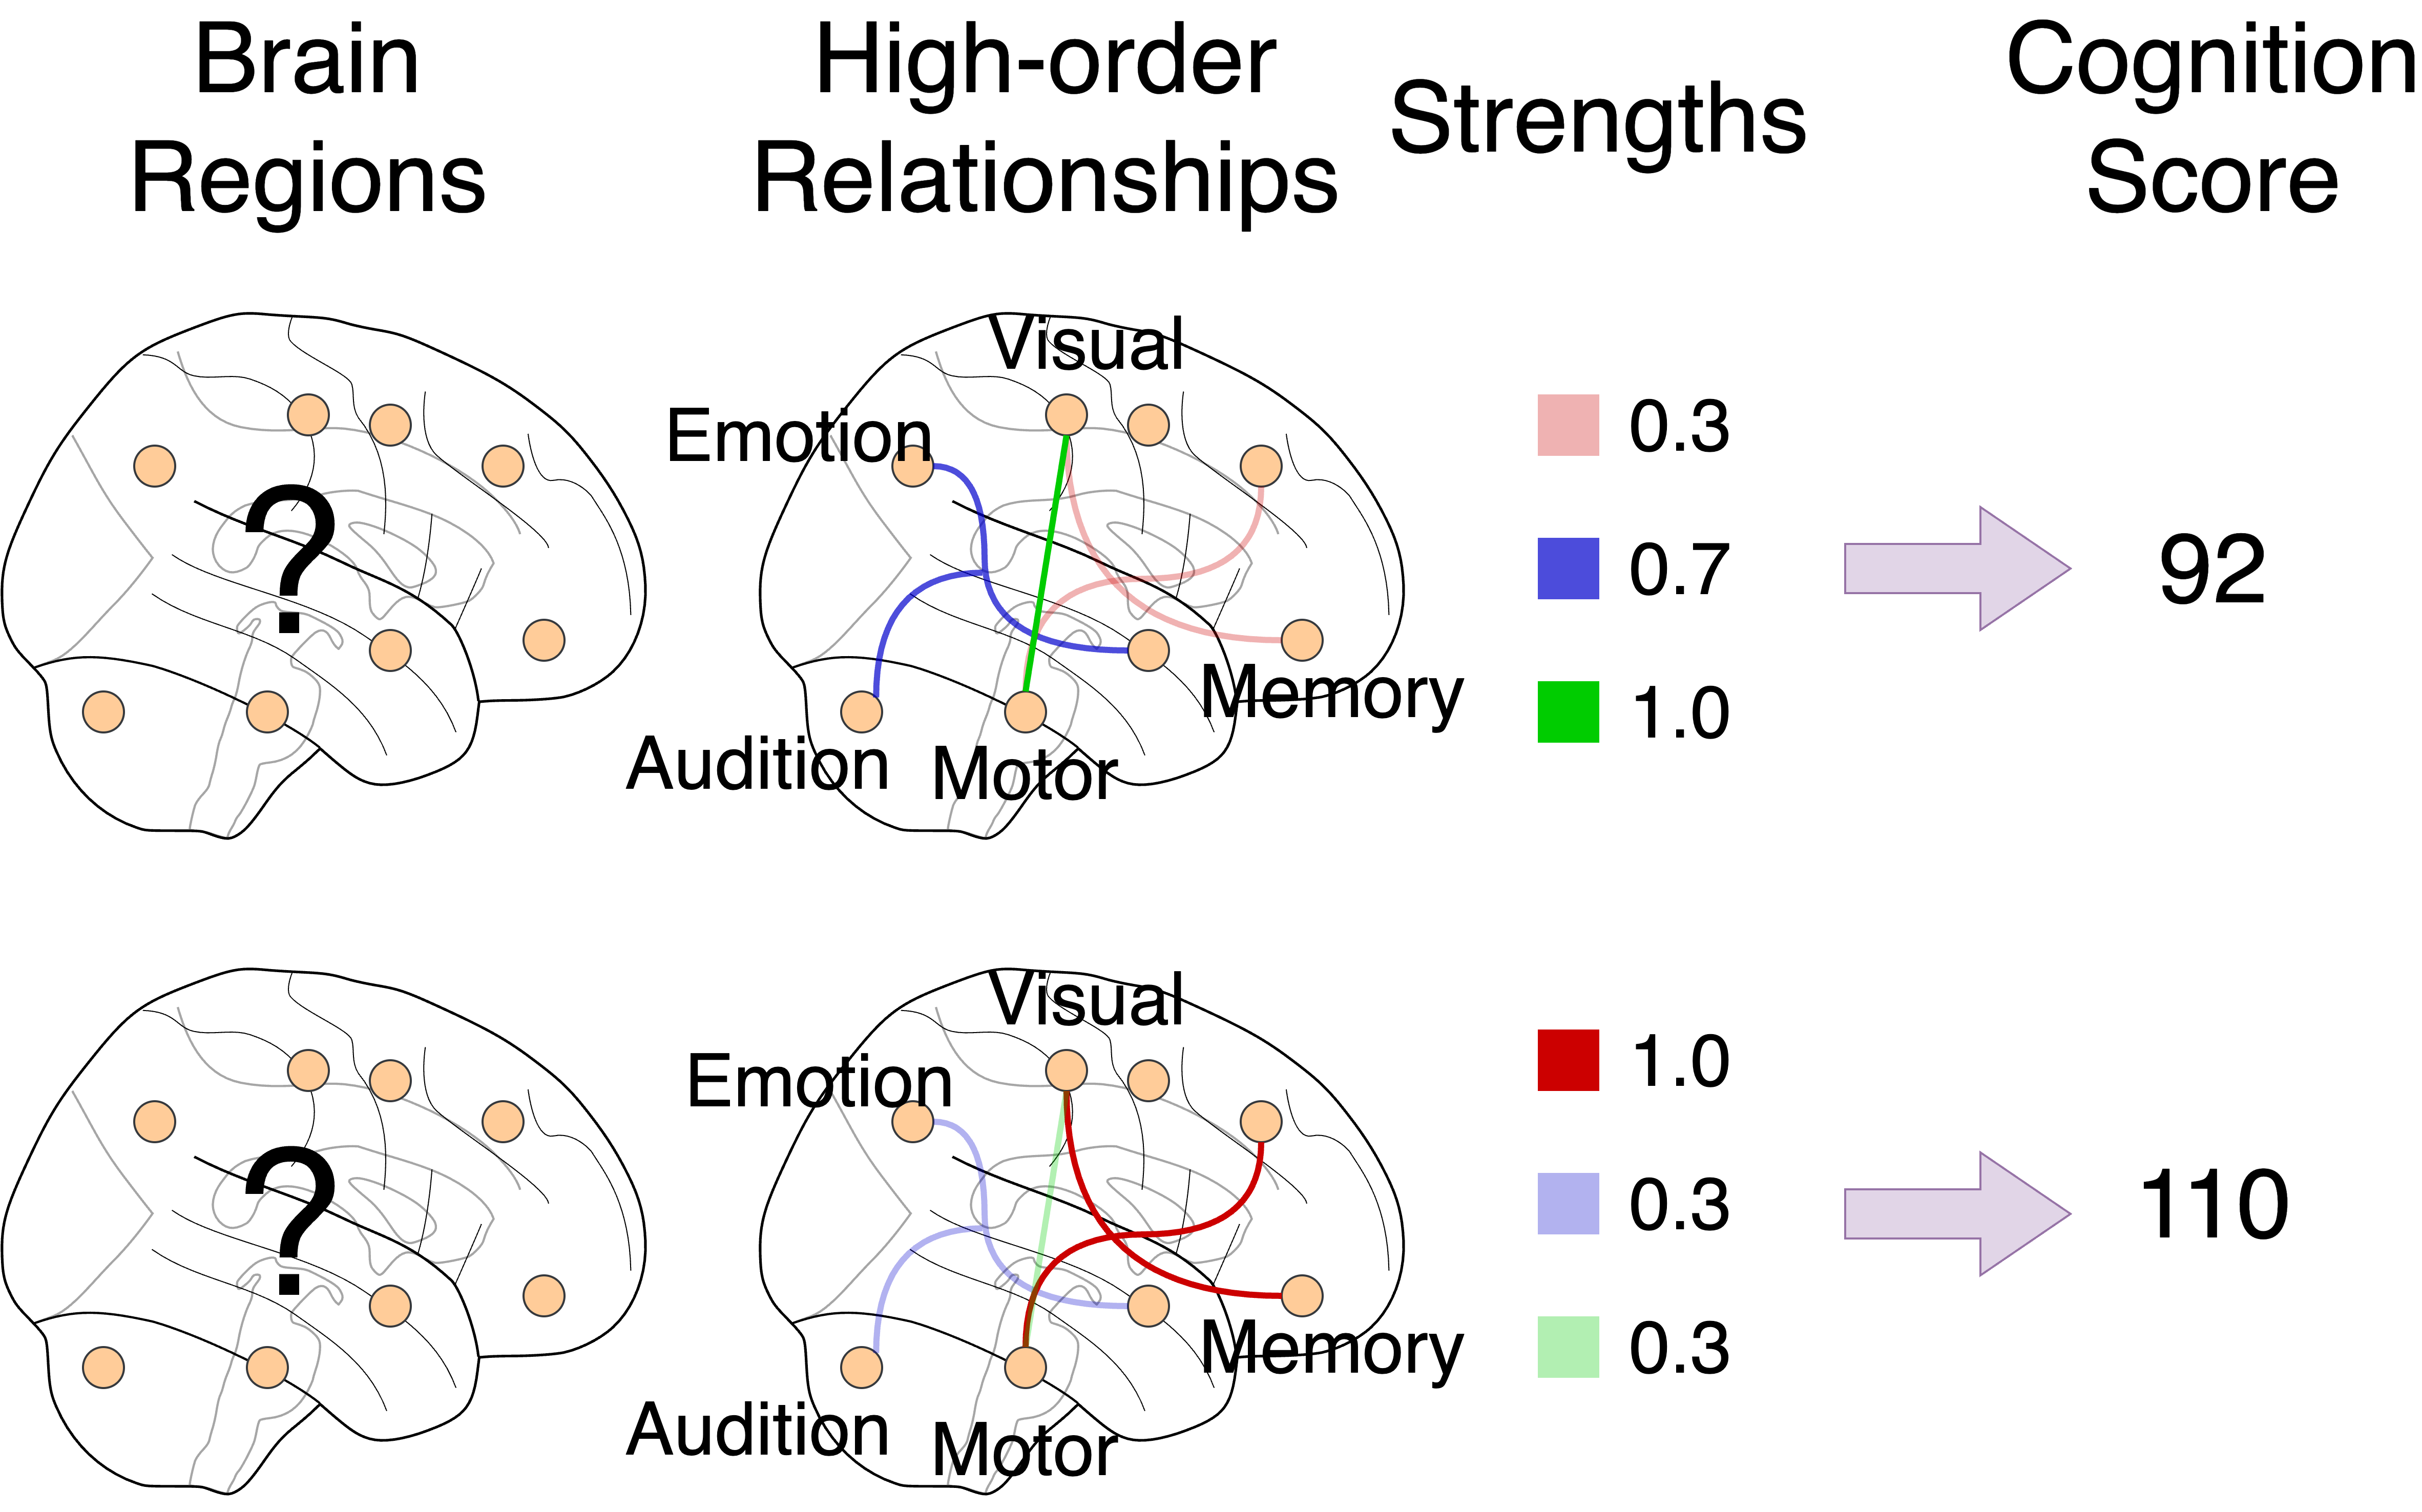
\includegraphics[width=\linewidth]{figures/tasting400.png}
    % \vskip 0.1in
    \caption{We identify high-order relationships of brain regions, where hyperedge structures and weights possess strong relevance to cognition (maximal informativeness). Meanwhile, they contain the least irrelevant information.}
    \label{fig:tasting}
% \vskip -0.1in
    
\end{figure}

% This property, on the one hand, ensures the high-order relationships encapsulate sufficient information related to cognition, which prevents the omission of any of them that makes a significant contribution to cognition. On the other hand, it allows us to diminish irrelevant ones, which will make the results as succinct as possible.


% \htl{we (propose to) formulate the capture of high-order relationship in the brain as the construction of the hypergraph, where the nodes are regions and the hyperedges connect all the related regions.}
% \htl{To better...(require a motivation of why MRMI), a desired hypergraph should maximize the correlation between hyperedges and the predicted property while diminishing the correlation with unrelated inputs, which is also demonstrated by xxx.}

% \htl{However, most of the previous works on hypergraph construction fail to xxx since }

We formulate high-order relationships as weighted hyperedges in a hypergraph, where regions are treated as nodes. Unlike a traditional graph where edges connect only two nodes, a hypergraph allows edges, known as hyperedges, to connect any number of nodes. The hypergraph should be weighted, and the weights of hyperedges are considered as strengths of high-order relationships, which contain the information relevant to the outcome (Figure \ref{fig:tasting}). 
% Therefore, our goal is to construct a weighted hypergraph model of each brain, where the nodes are regions and hyperedges are set to be identified. These hyperedges should be maximally informative and minimally redundant: \textit{informativeness} is the mutual information between the hyperedges and the prediction target (e.g. cognition score).
% We maximize it because we expect these hyperedges to carry more information about the target; \textit{redundancy} is the mutual information between the hyperedges and the inputs. We minimize it because we expect succinct relations. Acquiring such maximally informative and minimally redundant hyperedges is much more challenging than pairwise edges in a normal graph due to the exponential search space since the number of nodes connected by a hyperedge can be arbitrary.\htl{better to separate it into two sentences "...due to...since"}

% In addition, \stodo{perhaps ad
% isk of overfitting in the model.

However, current methods for hypergraph construction, which are mostly based on neighbor distances and neighbor reconstruction \citep{wang2015visual,liu2017elastic,jin2019robust,huang2009video}, are unsuitable in our context for several reasons: 1) they are unable to learn MIMR hyperedges due to the absence of a tractable objective for learning such hyperedges.  2) they fall short of learning consistent structures across subjects, which contradicts the belief that the cognitive function mechanism of healthy human beings should be similar \citep{wang2023inference}. 3) the number of hyperedges is restricted to the number of nodes, which may lead to sub-optimal performance. Furthermore, although information bottleneck (IB) has been a prevailing solution to learn MIMR representations in deep learning \citep{kim2021drop,alemi2016deep,luo2019significance}, existing IB methods focus on extracting compressed representations of inputs instead of identifying underlying structures such as hypergraphs. Harnessing the IB framework for identifying hypergraphs necessitates both architectural innovations and theoretical derivations.

\paragraph{Proposed Work} In this paper, we propose \textbf{Hy}pergraph of \textbf{B}rain \textbf{R}egions via mult\textbf{i}-head \textbf{D}rop-bottleneck (\mname{}), a novel approach for identifying maximally informative yet minimally redundant high-order relationships of brain regions. The overall pipeline of \mname{} is depicted in Figure \ref{fig:pipeline}. \mname{} is equipped with a \textsc{Constructor} and a \textsc{Weighter}. The \textsc{Constructor} identifies the hyperedge structures of brain regions by learning sets of masks, and the \textsc{Weighter} computes a weight for each hyperedge. To advance the IB principle for hyperedge identification, we further propose \textit{multi-head drop-bottleneck} and derive its optimization objective.

\mname{} avoids searching in an exponential space through learning masks to identify hyperedges, which guarantees efficiency. Its feature-agnostic masking mechanism design ensures \mname{} to learn consistent structures across subjects. Moreover, the model is equipped with a number of parallel heads, each of which is dedicated to a hyperedge. Through this, \mname{} is able to identify any number of hyperedges, depending on how many heads it is equipped with. Additionally, the proposed \multiheadname{} theoretically guarantees the maximal informativeness and minimal redundancy of the identified hyperedges. 

% To alleviate the data scarcity issue, \mname{} is equipped with a special architecture, where some components are shared by all datasets, and others are specific to the condition.

We evaluate our methods on the open-source ABIDE dataset and the restricted ABCD dataset. We quantitatively evaluate our approach by a commonly used protocol for studying brain connections, CPM~\citep{shen2017using} (Appendix \ref{sec:app_cpm}), and show that our model outperforms the state-of-the-art deep learning models by an average of $11.2\%$ on a comprehensive benchmark. Our post-hoc analysis demonstrates that hyperedges of higher degrees are considered more significant, which indicates the significance of high-order relationships in human brains.
\section{Problem Definition \& Notations}
\label{sec:hybrid-prelims}
% \subsection{Problem Definition \& Notations}
\paragraph{Input} 
 Our dataset is a collection of human subject's features and their phenotypic outcomes, which is represented by the pair $(X, Y)$ for each subject. $X \in \mathbb{R}^{N \times d}$ represents the features for each subject, where $N$ is the number of brain regions and $d$ is the feature size. Consistent with previous works \citep{kan2022brain,li2021braingnn}, the features are Pearson correlations derived from fMRI time series. $Y \in \mathbb{R}$ denotes the phenotypic outcome, such as the intelligent quotient. Full implementation details and hyperparameter settings are provided in \cite{qiu2023learning}.
 
 %For how to obtain features of regions from raw data, see for more details.

\paragraph{Goal}
Based on the input $X$, \hybrid{} aims to learn a weighted hypergraph of the brain, where regions are nodes. To achieve this, \hybrid{} identifies a collection of hyperedges $H = (\boldsymbol{h}^1, \boldsymbol{h}^2, \cdots, \boldsymbol{h}^K)$, and assigns weights $\boldsymbol{w} = [w^1, w^2, \cdots, w^K]^T$ for all hyperedges. These hyperedges and their weights, which represent strengths of hyperedges, are expected to be the most informative towards $Y$ yet the least redundant. 

\paragraph{Representation of Hyperedges}
As mentioned before, we use $H$ to denote the collection of hyperedge structures and $\boldsymbol{h}^k$ to denote the $k$-th hyperedge. To associate hyperedges with node memberships, we use the following representation for a hyperedge:
\begin{equation}
    \boldsymbol{h}^k = \boldsymbol{m}^k \odot X \in \mathbb{R}^{N\times d},
\end{equation}
where $\boldsymbol{m}^k \in \{0,1\}^N$ is a mask vector and $\odot$ denotes broadcasting element-wise multiplication. In other words, each $\boldsymbol{h}^k$ is a randomly row-zeroed version of $X$.
\section{Related Work}
\paragraph{Hypergraph Construction}
 Existing hypergraph construction methods are mostly based on neighbor reconstruction and neighbor distances. For example, the $k$ nearest neighbor-based method \citep{huang2009video} connects a centroid node and its $k$ nearest neighbors in the feature space to form a hyperedge. \citet{wang2015visual,liu2017elastic,jin2019robust,xiao2019multi} further refine these neighbor connections through various regularization. However, the number of hyperedges of these methods is restricted to the number of nodes, and hyperedges obtained by these methods are inconsistent across instances. 
 Cluster-based approaches learn community structure in a graph \cite{bannadabhavi2023community,ying2018hierarchical}, which can also be used to form hyperedges.
 \citet{zhang2022deep,zhang2018dynamic} proposed to iteratively refine a noisy hypergraph, which is obtained by the aforementioned methods. Therefore, they share the same limitations as the aforementioned methods. In addition, these methods are unable to learn MIMR hyperedges due to the absence of a tractable objective. Other methods, such as attributed-based methods~\citep{huang2015learning, joslyn2019high}, are ill-adapted to our context since they require discrete labels. 
 %or a prior graph topology, which is usually very noisy.
 Different from these methods, we provide a way to learn a consistent hypergraph through a deep-learning model. Furthermore, thanks to the proposed \multiheadname, these hyperedges are theoretically ensured MIMR.

\paragraph{High-Order Relationships in fMRI}

Although there are some methods working on high-order relationships in fMRI, they have limitations and are inconsistent with our MIMR objective.
\citet{xiao2019multi,li2022construction} used the existing non-learning-based hypergraph construction methods, which may lead to noisy and inexpressive hypergraphs. \citet{zu2016identifying,santoro2023higher} enumerated all hyperedges with degrees lower than 3, which can only discover a tiny portion of all possible hyperedges in exponential space and is not scalable to a large degree. \citet{rosas2019quantifying} proposed O-information, which reflects the balance between redundancy and synergy. The O-information metric is utilized by \citet{varley2023multivariate} to study fMRI data. However, the objective of these methods is not consistent with ours: although both of us are quantifying the redundancy of high-order relations, our method is to learn those that are most informative toward a cognition score, while theirs is to depict the synergy and redundancy within a system.

\paragraph{Information Bottleneck}
Information bottleneck (IB) \citep{tishby2000information} is a technique in data compression. The key idea is to extract a summary of data, which contains the most relevant information to the objective. \citet{alemi2016deep} first employed an IB view of deep learning. After that, IB has been widely used in deep learning. The applications span areas such as computer vision \citep{luo2019significance,peng2018variational}, reinforcement learning \citep{goyal2019infobot,igl2019generalization}, natural language processing \citep{wang2020learning} and graph learning \citep{yu2020graph,yu2022improving, xu2021infogcl,wu2020graph}. Unlike these studies that use IB to extract a compressed representation or a select set of features, our approach focuses on identifying the underlying structures of the data.

\paragraph{Connectivity-based Phenotypic Prediction}
Recently, deep learning techniques have been increasingly employed in predicting phenotypic outcomes based on the connectivity of brain regions. Most works \citep{ahmedt2021graph,li2019graph,cui2022interpretable,kan2022fbnetgen,cui2022braingb,said2023neurograph} model the brain network as a graph, in which regions act as nodes and pairwise correlations form the edges. These methods predominantly utilize Graph Neural Networks (GNNs) to capture the connectivity information for predictions. In addition to GNNs, \citet{kan2022brain} proposed to use transformers with a specially designed readout module, leveraging multi-head attention mechanisms to capture pairwise connectivity. However, all of these methods heavily rely on pairwise connectivity and neglect more intricate higher-order relationships. This oversight, on the one hand, leads to sub-optimal prediction performances and, on the other hand, prevents domain experts from acquiring insightful neuroscience interpretations, given that brain functions often involves multiple regions.
\section{Method}
\label{sec:hybrid-approach}
\paragraph{Method Overview}

\hybrid{} consists of a \textsc{Constructor} $\mathcal{F}_c$, a \textsc{Weighter} $\mathcal{F}_w$, and a \textsc{LinearHead} $\mathcal{F}_l$. At a high level, the \textsc{Constructor} $\mathcal{F}_c$ is responsible for identifying hyperedges $H$ from the data to construct the hypergraph. After that, the \textsc{Weighter} $\mathcal{F}_w$ calculates a weight for each hyperedge. Finally, based on all the weights $\boldsymbol{w}$, the \textsc{LinearHead} $\mathcal{F}_l$ predicts the label $Y$.
An illustration of this pipeline is shown in Figure \ref{fig:pipeline}. The pipeline can be formulated as
\begin{equation}
% \vspace{-1em}
    \label{equ:pipeline}
    X \xrightarrow[\mathcal{F}_c]{} H \xrightarrow[\mathcal{F}_w]{} \boldsymbol{w}\xrightarrow[\mathcal{F}_l]{} Y.
\end{equation}

We will elaborate on the details of the architecture below.

\begin{figure*}
\vspace{0.8em}
    \centering
    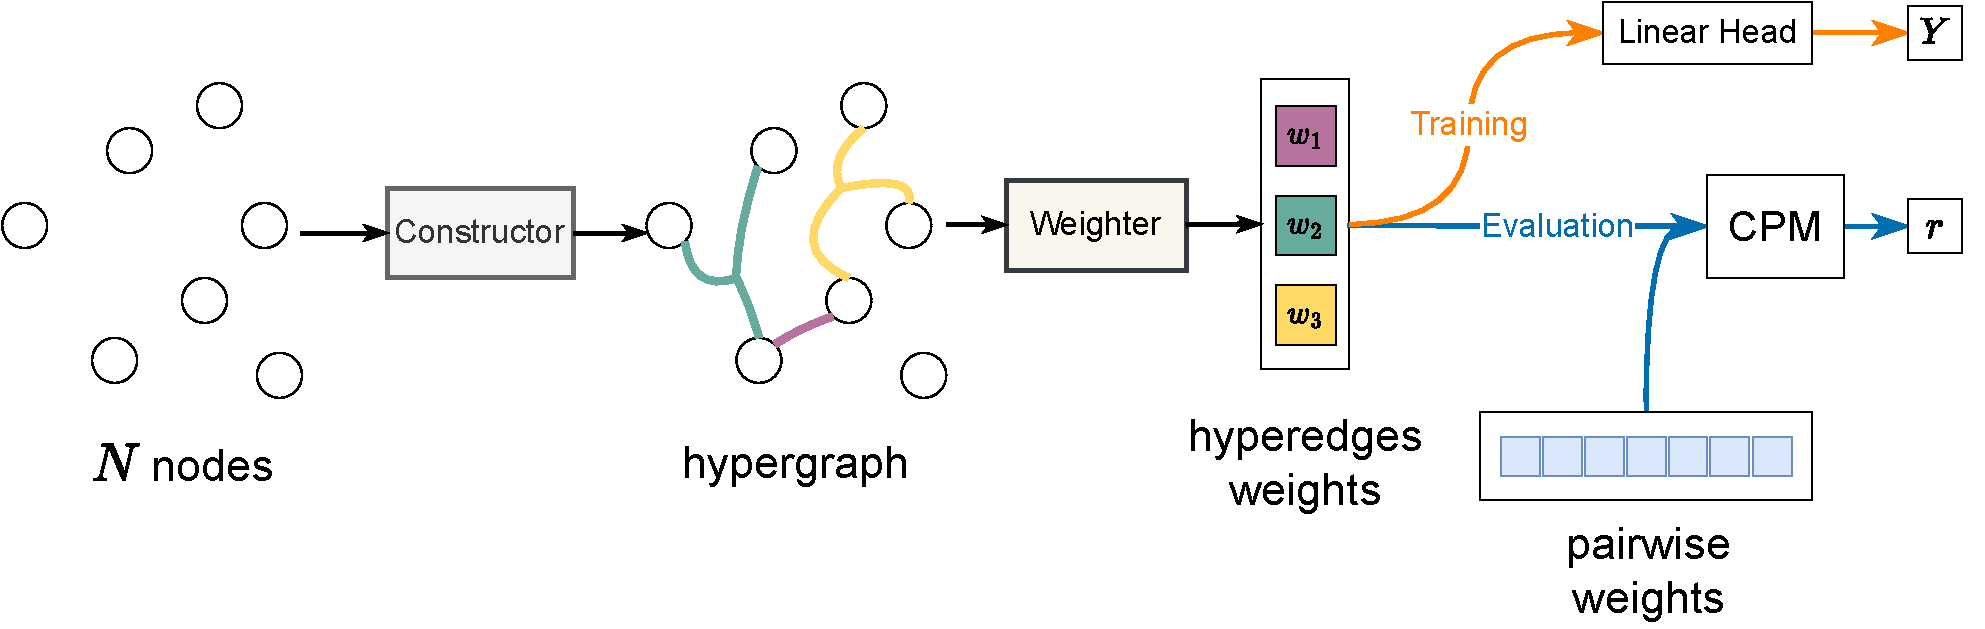
\includegraphics[width=\linewidth]{figures/pipeline2.drawio.pdf}
    % \vskip 0.1in
    \caption{Overview of the \hybrid{} pipeline when the total number of hyperedges $K=3$. Hyperedge are in distinct colors for clarity.  The \textsc{Constructor} identifies hyperedges in the hypergraph, where regions are nodes. The \textsc{Weighter} computes a weight for each hyperedge. These weights, representing strengths of hyperedges, are expected to be informative in terms of our target $Y$. There are two separate phases after obtaining weights of hyperedges: 1) Training. The model's parameters are trained under the supervision of $Y$; 2) Evaluation. The output weights, as well as pairwise weights, are fed into the CPM \citep{shen2017using}.}
    \label{fig:pipeline}
    % \vskip -0.1in
\end{figure*}

\subsection{Learning the Hypergraph by Multi-head Masking}
\label{sec:learn-by-mask}

Each instance (human subject) is represented by $X = [X_1, X_2, \cdots, X_N]^T \in \mathbb{R}^{N\times d}$, where $X_i \in \mathbb{R}^d$ is a column vector representing the features of region $i$. These regions are nodes in the hypergraph we are going to construct. Hyperedges in the hypergraph can be beneficial in the learning process below because it is essential to model the relationships between more than two regions.

\paragraph{Hyperedges Construction}
In this paragraph, we elaborate on how the \textsc{Constructor} identifies the hyperedges, i.e. $H=\mathcal{F}_c(X)$.

Suppose the number of hyperedges is $K$, which is a predefined hyperparameter. We assign a head to each hyperedge. Each head is responsible for constructing a hyperedge by selecting nodes belonging to that hyperedge. 

Specifically, to construct the $k$-th hyperedge, the \textsc{Constructor}'s $k$-th head outputs a column vector $\boldsymbol{m}^k \in \{0,1\}^N$, where each element in the vector corresponds to a brain region,

\begin{equation}
\label{equ:shallow}
% \begin{aligned}
\boldsymbol{m}^k = [\mathbbm{1}(p^k_{\theta,1}), \mathbbm{1}(p^k_{\theta,2}), \cdots, \mathbbm{1}(p^k_{\theta,N})]^T \in \{0, 1\}^N,
% \end{aligned}
\end{equation}
where $p^k_{\theta, i} \in [0,1], i=1,2,\cdots, N$ are learnable probabilities. $\mathbbm{1}: [0,1] \mapsto \{0,1\} $ is an indicator function, which is defined as $\mathbbm{1}(x) = 1$ if $x > 0.5$ and $\mathbbm{1}(x) = 0$ if $x \leq 0.5$.  And $\boldsymbol{m}^k$ is a column vector corresponding to the $k$-th hyperedge. Note that since there is no gradient defined for the indicator operation, we employ the stop-gradient technique \citep{oord2017neural,bengio2013estimating} to approximate it.

\begin{figure}[t]
    \centering
    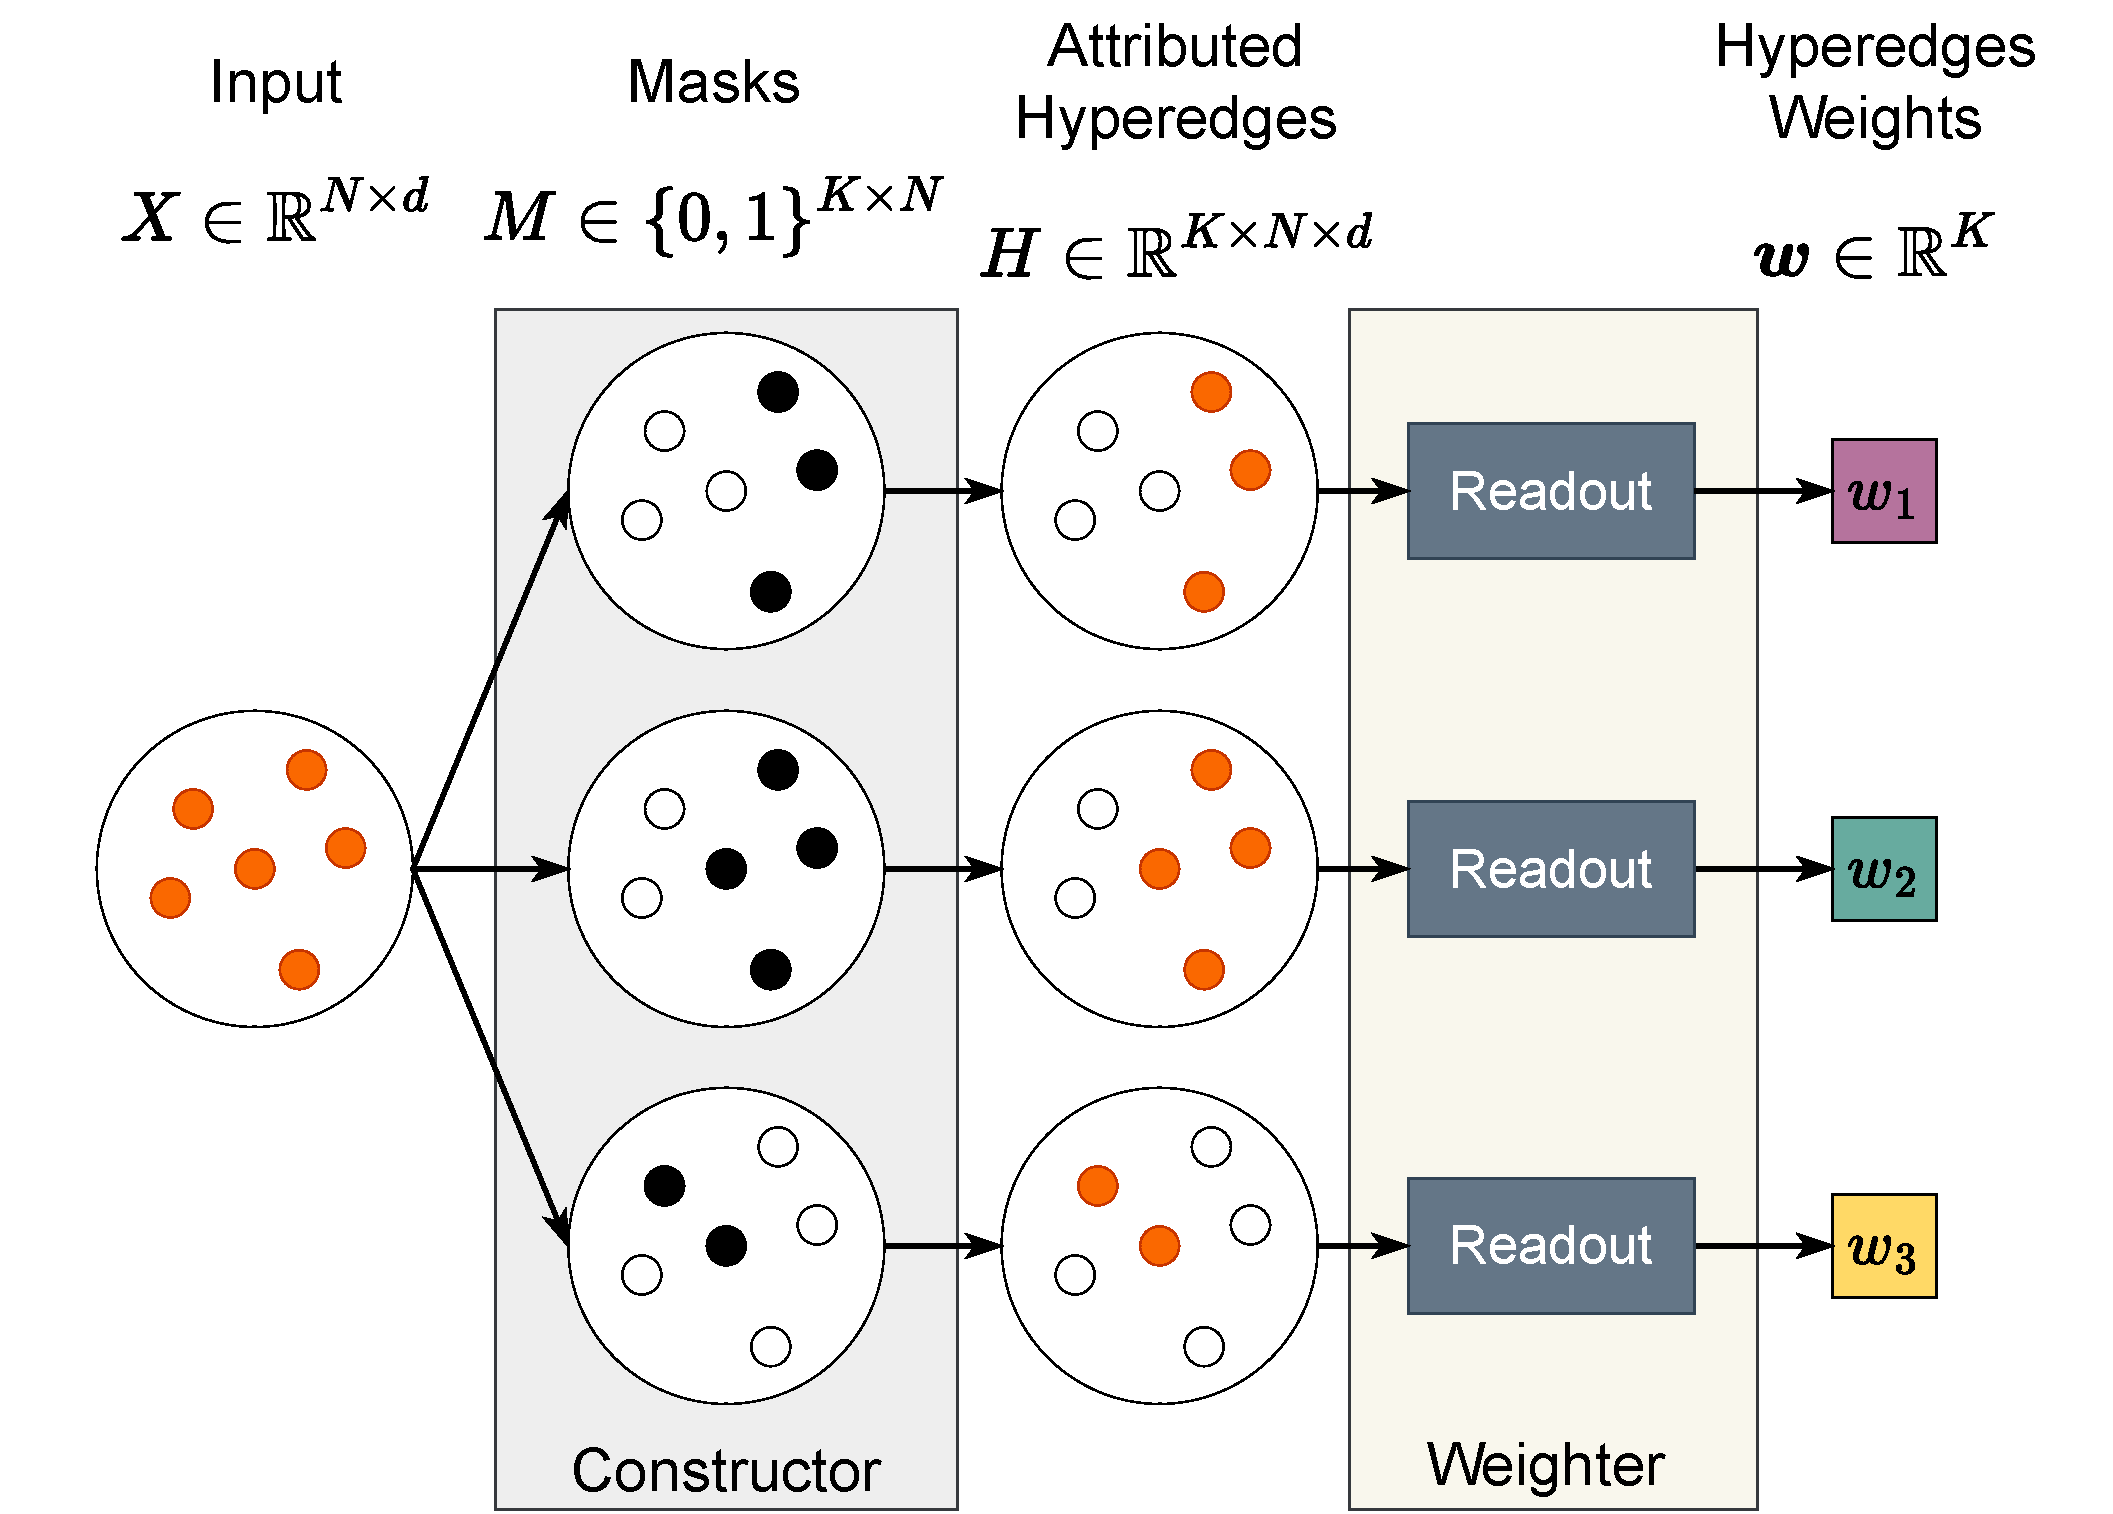
\includegraphics[width=0.63\linewidth]{figures/architecture.drawio.pdf}
    \caption{Architecture details of the \textsc{Constructor} and the \textsc{Weighter}  when the number of nodes $N=6$ and the number of hyperedges $K=3$. At a high level, the \textsc{Constructor} learns the hyperedge structure by masking nodes. The \textsc{Weighter} computes the weight of each hyperedge based on the hyperedge's member nodes and their features.}
    \label{fig:enter-label}
\end{figure}

In the vector $\boldsymbol{m}^k$, $0$ indicates nodes that are masked out, and $1$ indicates nodes that are not masked. Nodes that are not masked are considered to form a hyperedge together. We use $\boldsymbol{h}^k$ to represent the masked version of $X$
\begin{equation}
\begin{aligned}
    \boldsymbol{h}^k &= \boldsymbol{m}^k \odot X \\&= [\boldsymbol{m}^k_1 X_1, \boldsymbol{m}^k_2 X_2, \cdots, \boldsymbol{m}^k_N X_N] \in \mathbb{R}^{N\times d},   
\end{aligned}
\end{equation}
where $\odot$ is the broadcast element-wise multiplication. $\boldsymbol{m}^k_j$ is the $j$-th element of the vector $\boldsymbol{m}^k$.  

We obtain $K$ hyperedges for $K$ sets of masks. We use $H$ to denote the collection of all hyperedges.
\begin{equation}
    H = (\boldsymbol{h}^1, \boldsymbol{h}^2, \cdots, \boldsymbol{h}^K).
\end{equation} 

\paragraph{Hyperedge Weighting}
After obtaining the structure (i.e. member nodes) of each hyperedge,  the \textsc{Weighter} will calculate each hyperedge's weight, which is supposed to indicate the importance of that hyperedge, based on the member nodes and their features, i.e. $\boldsymbol{w} = \mathcal{F}_w(H)$.

These weights are obtained by a $\operatorname{Readout}$ module, which is composed of: 1) summing over all the non-masked nodes feature-wisely; 2) dim reduction operation.

\begin{equation}
\label{equ:readout}
    w^k = \operatorname{Readout}(\boldsymbol{h}^k) = \operatorname{DimReduction}({\boldsymbol{m}^k}^T\boldsymbol{h}^k) \in \mathbb{R},
\end{equation}

where $w^k$ is the weight of the $k$-th hyperedge and $\operatorname{DimReduction}$ is an MLP with ReLU activations, where the output dimension is $1$.
For all hyperedges, we obtain $K$ hyperedges in total, $\boldsymbol{w} = [w^1, w^2, \cdots, w^K]^T \in \mathbb{R}^K$. Finally, these weights will be fed into the final linear head to predict the label of the instance, 
\begin{equation}
\label{equ:linearhead}
    \hat{Y} = \mathcal{F}_l(\boldsymbol{w}) \in \mathbb{R}.
\end{equation}

In contrast to previous hypergraph construction methods \citep{jin2019robust,xiao2019multi}, which identify hyperedges by refining neighbors and simply aggregating node features, \hybrid{} makes these procedures learnable and thus is able to identify MIMR hyperedges in a data-driven way through expressive neural networks. The Full study that decides the number of hyperedges $K$ is provided in \cite{qiu2023learning}.

\paragraph{Computational Complexity}
The computational complexity of our model is $O(N^2K)$, which is just the same scale as that of MLPs even though we are addressing a more challenging task: identifying high-order relationships in an exponential space. Details of the complexity calculation can be found in \cite{qiu2023learning}


\subsection{Optimization Framework}
 Since there are no existing IB frameworks that can be applied in our context, we propose a new IB framework named \multiheadname{} to optimize \hybrid{}. To adopt an information bottleneck view of \hybrid{}, we consider $X$, $Y$ and $H$ are random variables in the Markovian chain $X \leftrightarrow Y \leftrightarrow H$. According to our MIMR objective, we optimize
\begin{equation}
\label{equ:ib2}
    \arg \max I(H; Y) - \beta I(H; X),
\end{equation}
where $I(\cdot ; \cdot)$ denotes the mutual information. $I(H; Y)$ corresponds to the informativeness and $I(H; X)$ corresponds to the redundancy. $\beta$ is a coefficient trading off informativeness and redundancy. Since optimizing the mutual information for high-dimensional continuous variables is intractable, we instead optimize the lower bound of Equation \ref{equ:ib2}. Specifically, for the first term (informativeness), it is easy to show
\begin{equation}
\label{equ:lowerbound}
\begin{aligned}
    I(H; Y) &= \mathbb{H}[Y] -  \mathbb{H}[{Y|H}] \\
    &=\mathbb{H}[Y] + \mathbb{E}_{p(Y, H)}[\log p(Y|H)] \\
    & = \mathbb{H}[Y] + \mathbb{E}_{p(Y, H)}[\log q_\phi(Y|H)] \\
    &\quad + \mathbb{E}_{p(H)}[\operatorname{KL}(p(Y|H)|q_\phi(Y|H))] \\
   & \geq \mathbb{H}[Y] + \mathbb{E}_{p(Y, H)}[\log q_\phi(Y|H)],
\end{aligned}
\end{equation}
where $\mathbb{H}[\cdot]$ is the entropy computation.
Since there is no learnable component in the entropy of $Y$, we only need to optimize the second term $\mathbb{E}_{p(Y, H)}[\log q_\phi(Y|H)]$. $q_\phi$ can be considered as a model that predicts $Y$ based on $H$, which essentially corresponds to $\mathcal{F}_l \circ \mathcal{F}_w$, where $\circ$ is the function composition. In practice, we set $q_\phi$ as a Gaussian model with variance $1$ as most probabilistic machine learning models do for continuous data modeling \citep{alemi2016deep,luo2019significance,peng2018variational,kingma2013auto}. 


For the second term (redundancy) in Equation \ref{equ:ib2}, we have

\begin{proposition}
    (Upper bound of $I(H;X)$ in \multiheadname{})
\begin{equation}
\label{equ:multi_drop}
    \begin{aligned}
        I(H; X) 
        \leq \sum_{k=1}^K
        I(\boldsymbol{h}^k; X)
        &\leq \sum_{k=1}^K \sum_{i=1}^N
        I(\boldsymbol{h}^k_i; X_i)\\
        &= \sum_{k=1}^K\sum_{i=1}^N \mathbb{H}[X_i] (1 - p^k_{\theta, i}),
    \end{aligned}
\end{equation}
\end{proposition}

where $\boldsymbol{h}^k_i$ and $X_i$  is the $i$-th row of $\boldsymbol{h}^k$ and $X$ respectively.  $p^k_{\theta,i}$ is the mask probability in Equation \ref{equ:shallow}. $\mathbb{H}$ is the entropy computation. The equality holds if and only if nodes are independent and hyperedges do not overlap. It's important to clarify that optimizing Equation \ref{equ:multi_drop} does not imply a penalty for overlaps. The second inequality is inspired by \cite{kim2021drop}. The proof of the proposition can be found in \citet{qiu2023learning}.


% \begin{equation}
%     \mathcal{F}_c(X) =  \mathbbm{1}(p_\theta) \odot X
% \end{equation}
% \begin{equation}
%     q_\phi (H) =\mathcal{F}_l \circ \mathcal{F}_w (H)
% \end{equation}
Therefore, instead of optimizing the intractable objective Equations \ref{equ:ib2}, we optimize its upper bound (i.e. loss function) according to Equations \ref{equ:lowerbound} and \ref{equ:multi_drop}.
\begin{equation}
\begin{aligned}
    \mathcal{L} &= \| Y - \mathcal{F}_l \circ \mathcal{F}_w \circ \mathcal{F}_c (X) \|_2^2 + \beta \sum_{k=1}^K\sum_{i=1}^N \mathbb{H}[X_i] (1 - p^k_{\theta,i}) \\&\geq - I(H, Y) + \beta I(H, X).
\end{aligned}
\end{equation}
In conclusion, The learnable components are the shallow embeddings in Equation \ref{equ:shallow}, the $\operatorname{DimReduction}$ MLP in Equation \ref{equ:readout} and the \textsc{LinearHead} $\mathcal{F}_l$ in Equation \ref{equ:linearhead}.
\section{Experiments}
\label{sec:hybrid-experiments}

In this section, we conduct experiments to validate the quality of the learned hyperedges in terms of the predictive performance towards the cognition phenotype outcome. Furthermore, we conduct ablation studies to validate the key components in our model. We also analyze our results both quantitatively and qualitatively.

\subsection{Predictive Performance of Hypereges}
% \begin{algorithm}
% \begin{algorithmic}
% \STATE    $d \gets \text{an random integer between } 2 \text{ and } 30. $

% \STATE $\mathcal{H} \gets \{\}$
% \FOR{$i = 1:d$}
% \STATE $h \gets \text{randomly sample } d \text{ nodes}$
% \STATE $\mathcal{H} \gets \mathcal{H} \cup \{h\}$
% \ENDFOR

% \FORALL{$h$ in $H$}
% \FORALL{node in $h$}

% \STATE $w \gets U(0, 1)$
% \STATE $x \gets U(0, 2w)$
% \STATE $y \gets y + $

% \ENDFOR
% \ENDFOR

% \end{algorithmic}

% \caption{The procedure to construct the synthetic dataset.}
% \label{alg:syn}
% \end{algorithm}


% \paragraph{Real-World Datasets}
\paragraph{Datasets}
\label{par:real_dataset}

We consider two fMRI datasets: 

1) \textit{Autism Brain Imaging Data Exchange (ABIDE)} \citep{craddock2013neuro} is an open-source dataset. This dataset involved resting-state fMRI of patients from 17 international sites, as well as the anatomical and phenotypic data. Regions are obtained by Craddock 200 atlas \citep{craddock2012whole}. We use the preprocessed version from the official website. For prediction targets, we choose three intelligence quotients: FIQ (full-scale intelligence), VIQ (verbal intelligence quotient), and PIQ (performance intelligence). 
%We aim to show our model's effectiveness on different cognition targets.

2) \textit{Adolescent Brain Cognitive Development (ABCD)} \citep{casey2018adolescent} is one of the largest public fMRI datasets. Access is limited and requires adherence to a rigorous data request procedure to acquire the data. The data is collected from $11,875$ children aged between 9 to 10 years old. The functional MRI (fMRI) data is collected from children when they were resting and when they performed three tasks (SST, EN-back, MID). We use the ABCD imaging data collected from the baseline (release 2.0) as well as the 2-year follow-up (release 3.0). In conclusion, we obtain $8$ sub-datasets (we refer to them as \textit{datasets} from now on) from $2$ timepoints under $4$ tasks. Regions are obtained by AAL3v1 atlas \citep{rolls2020automated}. For preprocess procedures of the ABCD dataset, please refer to \citet{qiu2023learning} for more details. For the prediction target, we consider fluid intelligence as our label. Fluid intelligence reflects the general mental ability and plays a fundamental role in various cognitive functions.
%We aim to show our model's effectiveness on different cognition targets
%Recent literature has seen success in predicting intelligence based on pairwise predictive modeling \citep{dubois2018resting,dubois2018distributed}, and we aim to improve the prediction accuracy of the current methods by involving high-order relationships on both resting-state and task-based data.

For region features, consistent with previous connectivity-based methods \citep{li2021braingnn,kan2022brain,ktena2018metric,said2023neurograph}, we use a region's Pearson correlation coefficients to all other regions as the region features.
% \paragraph{Features}
% \paragraph{Data preprocessing}
% \label{par:prepocessing}
% The raw fMRI data of an instance is represented in four dimensions (3 spatial dimensions + 1 temporal dimension), which can be imagined as a temporal sequence of 3D images. First, brain images are parceled into regions (or nodes) using the AAL3v1 atlas \citep{rolls2020automated}. Following previous works \citep{kan2022brain,li2021braingnn,thomas2022self}, each region's time series is obtained by averaging all voxels in that region. Consistent with previous connectivity-based methods \citep{li2021braingnn,kan2022brain,ktena2018metric,said2023neurograph}, for each region, we use its Pearson correlation coefficients to all regions as its features. We randomly split the data into train, validation, and test sets in a stratified fashion. The split ratio is 8:1:1.


\paragraph{Evaluation Metric}
To evaluate the quality of hyperedges obtained by \hybrid, we use CPM~\citep{shen2017using}, a standard model that could evaluate the relevance between the connectivity and the prediction target, due to its high impact in the community. 
In the original implementation of CPM, weights of pairwise edges are obtained by Pearson correlation between nodes. These weights, as pairwise connectivity, are fed into the CPM. CPM will output a metric that measures the overall correlation between edges and the prediction target, which can be considered as a measure of edge qualities. This process is formulated as 
\begin{equation}
\label{equ:metric0}
    r^\prime = \operatorname{CPM}(\boldsymbol{w}_p, Y),
\end{equation}
where $\boldsymbol{w}_p \in \mathbb{R}^{K_p}$ denotes the pairwise edge weights and $K_p$ is the total number of pairwise edges. $r^\prime$ is a metric that measures the quality of weights based on positive and negative correlations to the outcome. 

To evaluate the quality of the learned weights for our model, we replace the pairwise edge weights with the learned high-order weights $\boldsymbol{w}_h \in \mathbb{R}^{K_h}$, and thus adjust Equation \ref{equ:metric0} to 
\begin{equation}
\label{equ:metric}
    r = \operatorname{CPM}(\boldsymbol{w}_h, Y),
\end{equation}

% where $[\cdot \| \cdot]$ denotes the concatenation of two vectors. 
Comparing $r$ to $r^\prime$ reflects the quality of learned weights in terms of the prediction performance since it measures the overall correlation between weights and the prediction target. In our model, $\boldsymbol{w}_h = \boldsymbol{w}$, which is the learned hyperedge weights.

% The fMRI data is processed using BioImage Suite \citep{joshi2011unified} with the standard preprocessing procedures, such as slice time and motion correction, registration to the MNI template (see details in \cite{greene2018task} and \cite{horien2019individual}). We delete scans with more than 0.10 mm mean frame-to-frame displacement. 
% We use the ABCD imaging data collected from the baseline (release 2.0) as well as the 2-year follow-up (release 3.0). For each time point, we included children subjected to four conditions: 

% The fMRI data is processed using BioImage Suite \citep{joshi2011unified}. First, we performed motion correction and slice-time correction using SPM5; and via BioImage Suite, the data were registered to a standardized $3mm \times 3mm \times 3mm$ common space, where we generated masks representing white matter, gray matter, and cerebrospinal fluid (CSF) and computed the mean time courses for both white matter and CSF. We orthogonalized each gray matter time course with respect to the mean time courses of both white matter and CSF, and we orthogonalized each gray matter time course to the six motion-related signals via SPM5. We then applied a bandpass Butterworth filter with a frequency range of $0.02$Hz to $0.1$Hz to the orthogonalized time courses. We used a Gaussian kernel with a full-width at half-maximum (FWHM) of $6$mm to enhance spatial coherence and spatial smoothing. Lastly, we removed the linear trend from all signals in accordance with the methodology detailed in \cite{shenGroupwiseWholebrainParcellation2013}. We deleted scans with more than 0.10 mm mean frame-to-frame displacement. Additional details about the standard preprocessing procedures, such as slice time and motion correction, and registration to the MNI template can be found in \cite{greene2018task} and \cite{horien2019individual}. 

% For the prediction target, we consider fluid intelligence as our label. Fluid intelligence reflects the general mental ability and plays a fundamental role in various cognitive functions. Recent literature has seen success in predicting intelligence based on pairwise predictive modeling \citep{dubois2018resting,dubois2018distributed}, and we aim to improve the prediction accuracy of the current methods. 
\begin{table*}
\caption{$r$ values of our hyperedges compared to baselines on the ABCD dataset. Results are averaged over 10 runs. Deterministic methods do not have standard deviations.}
\label{tab:main}
% \vskip 0.1in
\resizebox{\linewidth}{!}{
\begin{tabular}{ccllllllll}
    \toprule
{Type} & {Model}& {SST 1} & {EN-back 1} & {MID 1}  & {Rest 1}& {SST 2} & {EN-back 2} & {MID 2} & {Rest 2} \\
         \midrule
Standard &pairwise& $0.113$ & $0.218$ &  $0.099$ & $0.164$  & $0.201$&$0.322$&$0.299$ & $0.289$ \\
\shline
\multirow{3}{*}{\shortstack{Hypergraph\\Construction}}
&$k$NN &  $0.115$ &  $0.268$ & $0.168$ &  $0.127$  & $0.257$&$0.266$&$0.238$ & $0.315$\\
&$l_1$ hypergraph  & $0.099$ &$0.223$  &  $0.125$ & $0.126$ &$0.145$&$0.295$&$0.242$& $0.259$\\
&$l_2$ hypergraph &$0.096_{\pm0.002}$  & $0.197_{\pm0.003}$ &  $0.118_{\pm0.003}$ & $0.157_{\pm0.016}$ &$0.203_{\pm0.005}$&$0.272_{\pm0.004}$&$0.289_{\pm0.011}$&$0.307_{\pm0.006}$\\
\shline
\multirow{4}{*}{\shortstack{Connectivity\\based\\Prediction}}
&BrainNetGNN &  $0.227_{\pm0.060}$ & $0.287_{\pm0.043}$ &$0.266_{\pm0.046}$ & $0.221_{\pm0.040}$ &$0.468_{\pm0.058}$&$0.480_{\pm0.068}$& $0.506_{\pm0.057}$&$0.453_{\pm0.028}$\\
&BrainGB & $0.190_{\pm0.073}$ & $0.214_{\pm0.051}$ &$0.265_{\pm0.048}$& $0.176_{\pm0.066}$ & $0.447_{\pm0.089}$ & $0.483_{\pm0.077}$ &$0.458_{\pm0.064}$ & $0.432_{\pm0.076}$\\
&BrainGNN & $0.262_{\pm0.030}$ & $0.235_{\pm0.032}$ &  $0.260_{\pm0.049}$ & $0.185_{\pm0.058}$ & $0.455_{\pm0.028}$ & $0.391_{\pm0.077}$&$0.445_{\pm0.078}$ &$0.368_{\pm0.041}$\\
&BrainNetTF &$\underline{0.327_{\pm 0.084}}$ & $\underline{0.338_{\pm 0.056}}$  & $\underline{0.370_{\pm 0.098}}$ & $\mathbf{0.334_{\pm 0.084}}$ & $\underline{0.633_{\pm0.178}}$& $\underline{0.631_{\pm0.142}}$ & $\underline{0.629_{\pm0.123}}$ & $\underline{0.588_{\pm0.138}}$ \\ 
\shline
Ours  & \hybrid & $\mathbf{0.361_{\pm0.058}}$  & $\mathbf{0.348_{\pm0.061}}$ & $\mathbf{0.386_{\pm0.060}}$ &  $\underline{0.223_{\pm0.056}}$ &$\mathbf{0.738_{\pm0.054}}$ & $\mathbf{0.714_{\pm0.037}}$&$\mathbf{0.816_{\pm0.053}}$ &$\mathbf{0.730_{\pm0.049}}$\\
         \bottomrule
    \end{tabular}}
% \vspace{-0.5em}
\end{table*}

 
\begin{table}[t]
 \caption{$r$ values of our hyperedges compared to baselines on the ABIDE dataset. Results are averaged over 10 runs. Deterministic methods do not have standard deviations.}
    \label{tab:abide}
% \vskip 0.1in
\centering
    % \resizebox{\linewidth}{!}{
    \begin{tabular}{cclll}
    \toprule
      {Type} & {Model} & {FIQ} & {VIQ} & {PIQ}  \\
      \midrule
        Standard & pairwise & $0.052$ & $0.124$ & $0.056$ \\
        \shline
        \multirow{3}{*}{\shortstack{Hypergraph\\Construction}}
        & $k$NN & $0.023$ & $0.093$ & $0.056$ \\
        & $l_1$ hypergraph & $0.043$ & $0.125$ & $0.061$ \\
        & $l_2$ hypergraph & $0.148_{\pm0.000}$ & $0.141_{\pm0.014}$ & $0.063_{\pm0.004}$ \\
        \shline
        \multirow{4}{*}{\shortstack{Connectivity\\based\\Prediction}}
        &BrainNetGNN & $\underline{0.162_{\pm0.042}}$ & $\underline{0.199_{\pm0.042}}$ & $\underline{0.223_{\pm0.025}}$ \\
        &BrainGB & $0.125_{\pm0.119}$ & $0.154_{\pm0.068}$ & $0.157_{\pm0.053}$ \\
        &BrainGNN & $0.105_{\pm0.041}$ & $0.176_{\pm0.049}$ & $0.159_{\pm0.051}$ \\
        &BrainNetTF & $0.132_{\pm0.111}$ & $0.176_{\pm0.053}$ & $0.180_{\pm0.054}$ \\ 
        \shline
        Ours  & \hybrid & $\mathbf{0.181_{\pm0.040}}$ & $\mathbf{0.204_{\pm0.031}}$ & $\mathbf{0.245_{\pm0.042}}$\\
     \bottomrule
    \end{tabular}
    % }
\end{table}

\begin{table*}[t]
\caption{Ablation studies on the masking mechanism. Results are averaged over 10 runs.}
% \vskip 0.1in
\label{tab:ablation_mask}
\resizebox{\linewidth}{!}{
\begin{tabular}{cccccccccccc}
    \toprule
{Model} & {SST 1} & {EN-back 1} & {MID 1} &{Rest 1}& {SST 2} & {EN-back 2} & {MID 2}  &{Rest 2}\\
         \midrule
 \hybrid  & $\mathbf{0.361_{\pm0.058}}$ &$\mathbf{0.348_{\pm0.061}}$ & $\mathbf{0.386_{\pm0.060}}$ & $\underline{0.223_{\pm0.056}}$ &$\mathbf{0.738_{\pm0.054}}$& $\mathbf{0.714_{\pm0.037}}$ &  $\mathbf{0.816_{\pm0.053}}$ & $\mathbf{0.730_{\pm0.049}}$\\
 \hybrid$_\mathrm{NoMask}$  & $0.297_{\pm0.035}$ & $0.274_{\pm0.057}$ & $\underline{0.323_{\pm0.059}}$& $0.221_{\pm0.034}$&$0.653_{\pm0.036}$&$0.599_{\pm0.059}$ &$0.757_{\pm0.021}$ &$0.543_{\pm0.038}$\\
 \hybrid$_\mathrm{RndMask}$  & $0.256_{\pm0.069}$ & $0.191_{\pm0.046}$ & $0.255_{\pm0.080}$ & $0.190_{\pm0.051}$ &$0.541_{\pm0.069}$& $0.514_{\pm0.038}$&$0.598_{\pm0.064}$ &$0.482_{\pm0.083}$\\
 \hybrid$_\mathrm{SoftMask}$  & $\underline{0.343_{\pm0.042}}$ & $\underline{0.314_{\pm0.040}}$ & $0.320_{\pm0.055}$& $\mathbf{0.245_{\pm0.061}}$ &$\underline{0.707_{\pm0.042}}$ &$\underline{0.662_{\pm0.058}}$&$\underline{0.796_{\pm0.031}}$ & $\underline{0.655_{\pm0.030}}$ \\
         \bottomrule
    \end{tabular}}
    % \vspace{-0.6em}
\end{table*}

\paragraph{Baselines}
We compare our method with $3$ classes of baselines: 1) \textit{standard} method, which is exactly the classical method that predicts outcomes based on pairwise edges \citep{shen2017using, DADI2019115, bhaa407}. The comparison with standard methods shows whether the high-order connectivity has its advantage over the classical pairwise one or not. 
2) \textit{hypergraph construction} methods. We consider $k$NN \citep{huang2009video}, $l_1$ hypergraph \citep{wang2015visual}, and $l_2$ hypergraph \citep{jin2019robust}.
3) \textit{connectivity-based  phenotypic prediction} methods, which are state-of-the-art predictive models based on brain connectivity. We consider BrainNetGNN \citep{mahmood2021deep}, BrainGNN \citep{li2021braingnn}, and BrainNetTF \citep{kan2022brain}. BrainGB \citep{cui2022braingb} is a study of different brain graph neural network designs and we include its best design as a baseline. Since none of these models are able to identify hyperedge structures of brain regions, we input their last layer embeddings (each entry as a weight) into the CPM model. Note that our weights $\boldsymbol{w}$ are also last layer embeddings in \hybrid{}.

% \subsection{Results}

% \paragraph{Quality of Hyperedges}
\paragraph{Results}
We report $r$ values by CPM in Table \ref{tab:abide} and Table \ref{tab:main}. As we can see, on the ABIDE dataset, \hybrid{} consistently outperforms all the baselines on different targets, with an average improvement of $8.8\%$ compared to the state-of-the-art model.
On the ABCD dataset, \hybrid{} outperforms the state-of-the-art predictive models on $7$ datasets of ABCD, with an average improvement of \avgimp{}. The results demonstrate our model is able to learn informative hyperedges towards different phenotypic outcomes from fMRI data of various brain states. Rest 1 is the only dataset that our model reaches the second-best.

Further, the comparison between our model and the pairwise baseline demonstrates the superiority of incorporating high-order relationships over relying solely on pairwise ones.

\paragraph{Runtime} \hybrid{} outperforms all other deep learning baselines in efficiency, with $87\%$ faster than the second-fastest one (BrainNetTF). Full runtime analysis is provided in \citet{qiu2023learning}.

\paragraph{Ablation Studies}
We conduct an ablation study on the effect of our masking mechanism. Specifically, we compare our model with $3$ variants: 1) \hybrid$_\mathrm{RndMask}$: Replace the learnable masks with random masks with the same sparsity, initialized at the beginning of training. 2) \hybrid$_\mathrm{NoMask}$: Do not mask at all, which means all nodes and their features are visible to each head. 3) \hybrid$_\mathrm{SoftMask}$: Remove the indicator function and use $p^k_{\theta, i}$ directly in Equation \ref{equ:shallow}. Ablation results are shown in Table \ref{tab:ablation_mask}. We find the original \hybrid{} and the \hybrid$_\mathrm{SoftMask}$ outperform all other variants, which demonstrates the effect of learnable masks. Moreover, the original \hybrid{} is better than its soft version \hybrid$_\mathrm{SoftMask}$, which demonstrates our sparse and succinct representations preserve better information than smooth ones.

\paragraph{Additional Experiments on Synthetic Dataset}
Since there are no ground-truth hyperedges in real-world datasets of learning informative hyperedges towards a specific outcome, we construct a synthetic dataset to verify if our model can recover the correct hyperedge structure under the MIMR objective. We use the precision, recall, and F1 score to measure the correctness of the learned hyperedges with respect to the ground truth. Although it is challenging to learn hyperedges when only supervised by the task label, we find that our model reaches high performances, with an average improvement of 28.3\% in terms of the F1 score, compared to the strongest baselines.


\subsection{Further Analysis}
% \subsubsection{Hyperedge Profiles}
In this subsection, we analyze the results of our model. We mainly use the ABCD dataset in the analysis since it is much larger than the ABIDE dataset.
\paragraph{Hyperedge Degree Distribution}
We plot the hyperedge degree distribution in Figure \ref{fig:degree_dist}. We find there are two distinct clusters in the figure. The first cluster is hyperedges with degree $\leq 5$. $1$-degree and $2$-degree hyperedges are special cases of our method: $1$-degree hyperedges are individual nodes, which imply the contribution of individual regions to the cognition. $2$-degree hyperedges reveal the importance of traditional pairwise connectivity. The other cluster concentrates around degree $25$, which implies the importance of relationships of multiple regions.

\begin{figure*}
% \vspace{-0.5em}
\begin{center}
    \begin{subfigure}[t]{0.32\textwidth}
        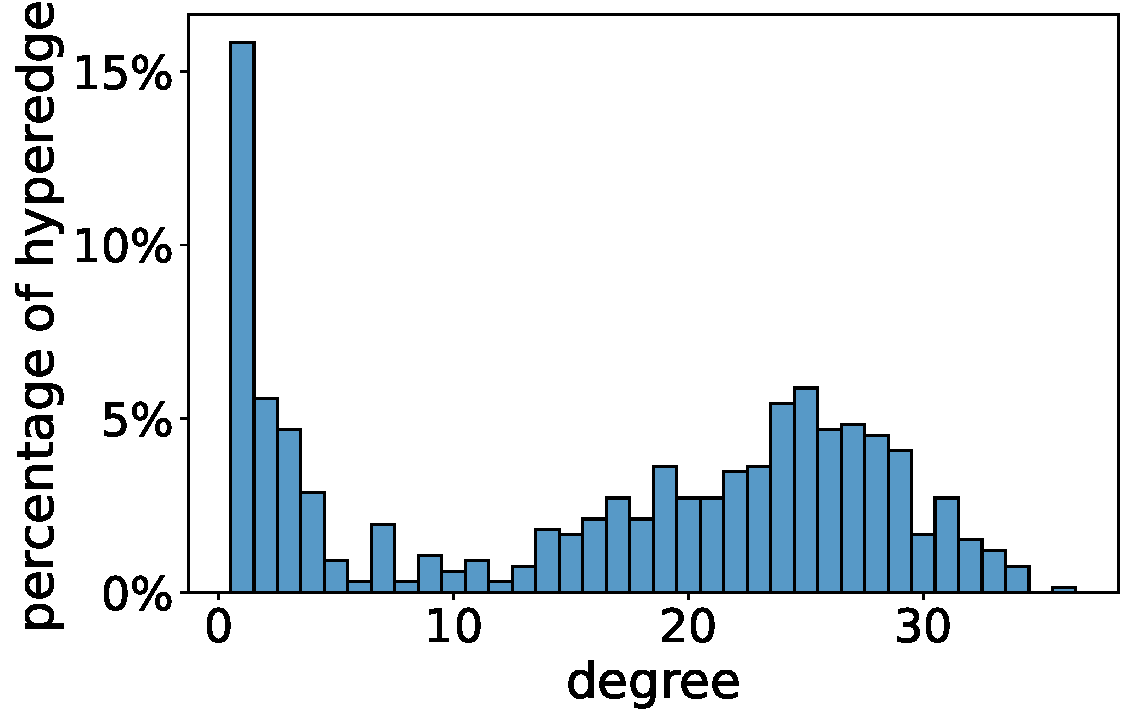
\includegraphics[width=\textwidth]{figures/degree_dist2.pdf}
        \caption{}
        \label{fig:degree_dist}
    \end{subfigure}
    \hspace{1em}
    \begin{subfigure}[t]{0.27\textwidth}
        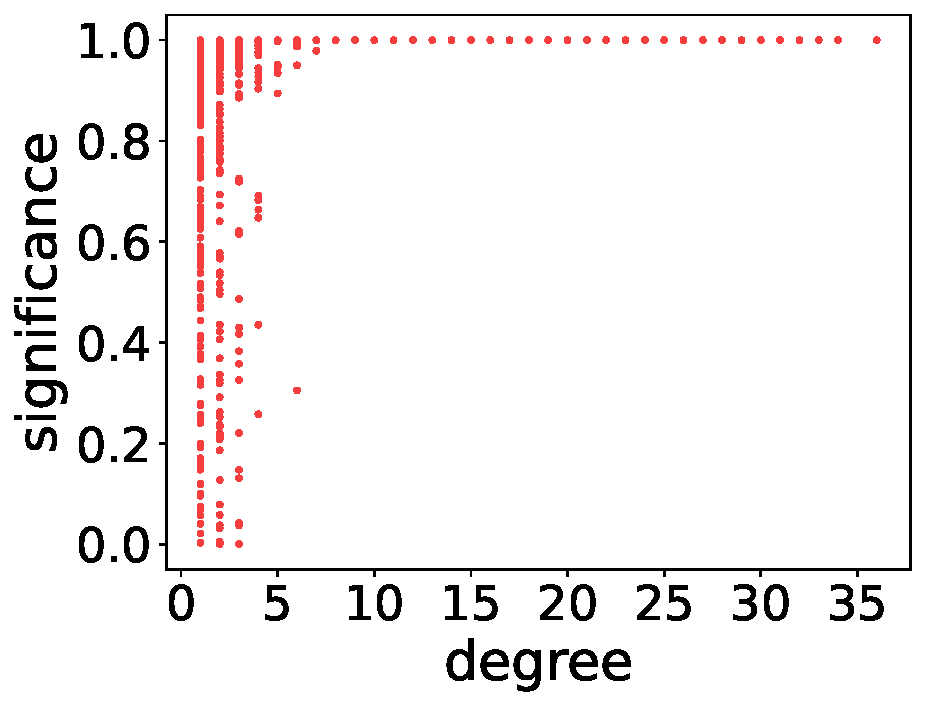
\includegraphics[width=\textwidth]{figures/degree_sig.pdf}
        \caption{}
        \label{fig:degree_sig}
    \end{subfigure}
        \hspace{1em}
    \begin{subfigure}[t]{0.28\textwidth}
        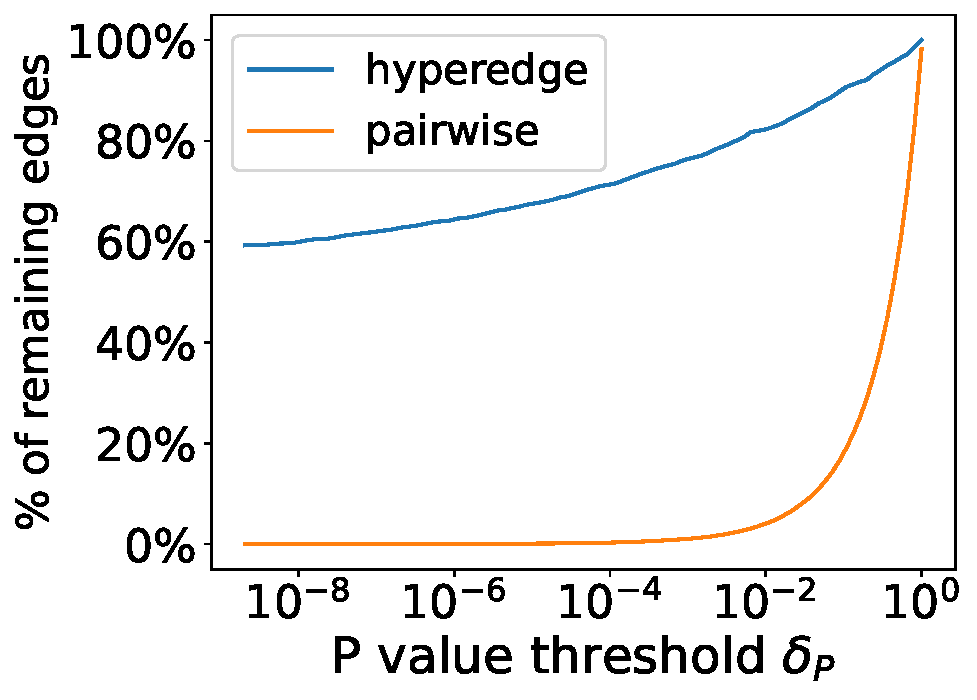
\includegraphics[width=\textwidth]{figures/num_sig.pdf}
        \caption{}
        \label{fig:cmp_sig_pair}
    \end{subfigure}
    % \vskip 0.1in
    \caption{Hyperedge profiles. \textbf{(a)} Hyperedge degree distribution of learned hyperedges. \textbf{(b)} Correlation between hyperedge degree and significance. \textbf{(c)} Comparison between the number of hyperedges and pairwise edges under different significance thresholds. The total number of hyperedges is $32$. And the total number of pairwise edges is $26,896$.}
    \label{fig:hyperedge_profile}
    % \vskip -0.1in
    \end{center}
\end{figure*}

% To further understand the relationship between hyperedge degree and its significance, we next plot their correlation in Figure \ref{fig:degree_sig}. \jialin{can be removed}
% \begin{wrapfigure}{R}{0.49\textwidth}
%           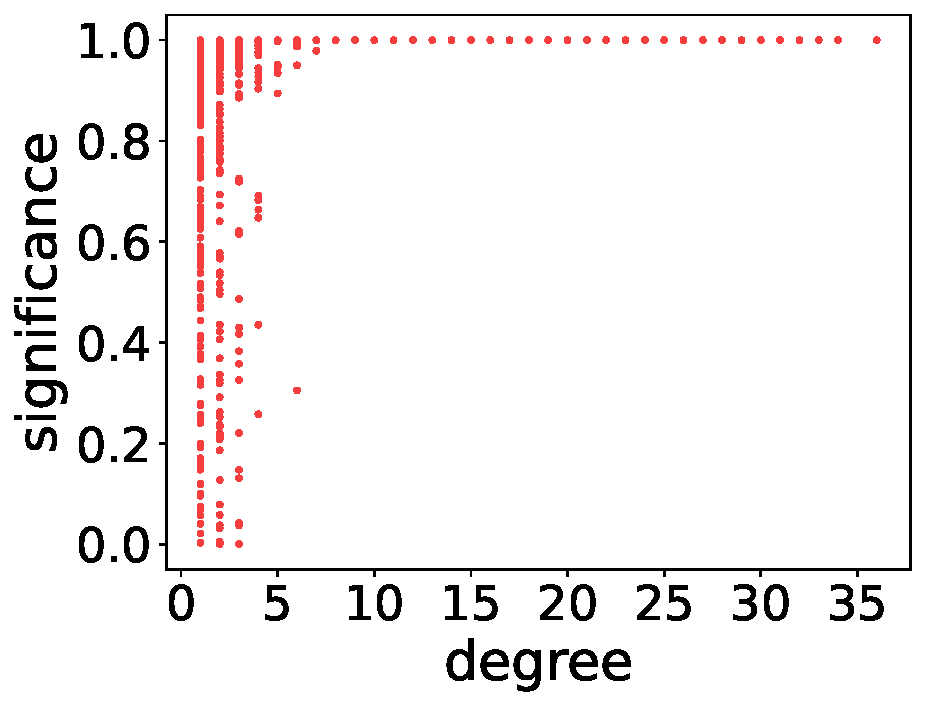
\includegraphics[width=\linewidth]{figures/degree_sig.pdf}
%     \caption{Relationship between the significances and degrees of learned hyperedges.}
%     \label{fig:degree_sig}
% \end{wrapfigure}

\paragraph{Hyperedges with Higher Degree are More Significant}
Since CPM conducts a significance test on pairwise edges and hyperedges internally based on a linear regression model, we can obtain a P-value for each hyperedge from the significance test. We define the significance of a hyperedge as $1-P_v \in [0, 1]$ where $P_v$ is the P-value of that hyperedge.

The relationship between hyperedge degree and its significance is shown in Figure ~\ref{fig:degree_sig}. In this figure, we find a strong positive correlation between a hyperedge's degree and its significance, which indicates that interactions of multiple brain regions play more important roles in cognition than pairwise or individual ones. It is also worth mentioning that there is a turning point around degree $5$, which corresponds to the valley around $5$ in Figure \ref{fig:degree_dist}.

\paragraph{High-order relationships are Better than Pairwise Ones}
To compare the significance in cognition between pairwise edges and learned hyperedges, we plot the number of remaining edges under different thresholds in Figure \ref{fig:cmp_sig_pair}. We find out that the learned hyperedges are much more significant than pairwise ones. Also note that even if we set the threshold to an extremely strict value ($1\times 10^{-8}$), there are still $60\%$ hyperedges considered significant. This evidence shows that our high-order relationships are much more significant than the traditional pairwise connectivity, which implies relationships involving multiple brain regions could be much more essential in cognition.


\paragraph{Hyperedge Case Study} We visualize the most significant hyperedge of the EN-back task in Figure \ref{fig:hyperedge1}. We observe a coordinated interaction of numerous brain regions, each fulfilling specific roles. Notably, some of these regions serve multi-functional purposes:
\begin{figure*}
    \centering
    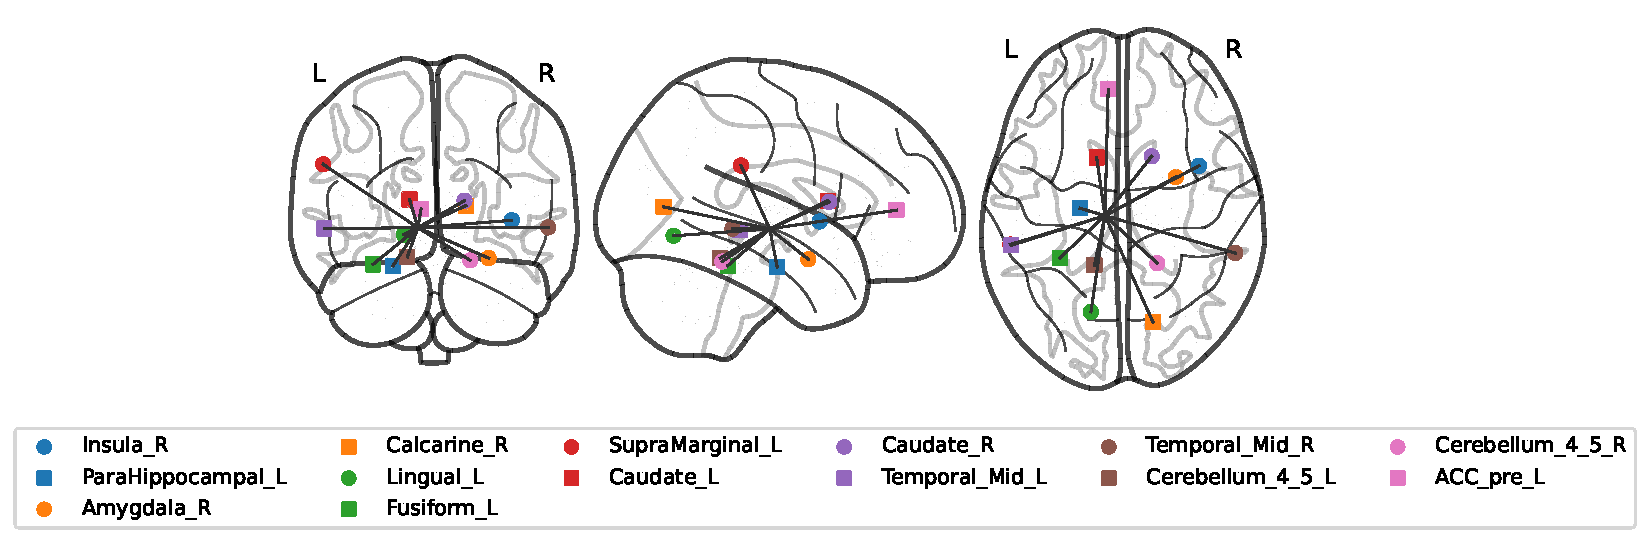
\includegraphics[width=\linewidth]{figures/hyperedge1.pdf}
    \caption{Visualization of the most significant hyperedge of the EN-back task.}
    \label{fig:hyperedge1}
\end{figure*}


\begin{itemize}
\item \textbf{Memory Processing} \textit{ParaHippocampal\_L}, \textit{Temporal Mid}: Essential for memory encoding and retrieval, these regions are integral to the EN-back task, facilitating the recall of previously viewed images.

\item \textbf{Emotional Processing} \textit{Amygdala\_R}: The amygdala is crucial for the processing of emotions, such as fear and pleasure. Since the EN-back task involves emotional stimuli, it is reasonable that the region is connected by the hyperedge.

\item \textbf{Visual Processing}: \textit{Calcarine\_R}, \textit{Lingual\_L}, \textit{Fusiform\_L}. These regions are responsible for visual perception and some of them are related to complex visual contents like symbols and human faces, which were presented during the fMRI task.

\item \textbf{Sensory} \textit{SupraMarginal\_L}: It is responsible for interpreting tactile sensors and perceiving limbs location. Its involvement is likely due to the requirement for participants to engage in specific physical actions, such as pressing buttons, during the task. \textit{Temporal Mid}: It functions in multi-modal sensory integration.

\item \textbf{Motor Control} \textit{Cerebellum}: It is primarily responsible for muscle control. \textit{Caudate}: It plays a crucial role in motor processes.  Its involvement is likely attributed to participants engaging in physical actions, like pressing buttons.

\item \textbf{Cognitive Control} \textit{ACC\_pre\_L}:  In the EN-back task, this region is likely crucial for maintaining focus, error detection and correction, conflict management in working memory, and modulating emotional responses to the task's demands.
\end{itemize}
\section{Conclusion}
In this work, we proposed \hybrid{} for identifying maximally informative yet minimally redundant (MIMR) high-order relationships of brain regions. To effectively optimize our model, we further proposed a novel information bottleneck framework and derived its theory. Our method outperforms state-of-the-art models. The result analysis shows the effectiveness of our model. We expect such advancements could benefit clinical studies, providing insights into neurological disorders, and offering improved diagnostic tools in neurology and other related fields.
\paragraph{Limitations}
\hybrid{} only considers static high-order relations. Given that fMRI tasks are dynamic, including temporal changes and interactions, it will be interesting to study the evolution of these high-order relationships.

Additionally, \hybrid{} does not offer a method for interpreting complex high-order relationships. This limitation is not specific to \hybrid{}, but is a common challenge in analyzing such relationships.




   \addcontentsline{toc}{chapter}{Bibliography} % To get an entry in the TOC.
    \setstretch{1.0}
    
    \bibliographystyle{plainnat}
    \bibliography{bibfile}



\end{document}